\documentclass[UTF8,10pt,a4paper]{ctexbook}
\def\mlbook{}
\providecommand{\pathroot}{.}
\usepackage{minted}
\usepackage{amsfonts}
\usepackage{amsmath}
\usepackage{CJK,CJKnumb}

\usepackage{fontspec}
\usepackage{geometry}
\geometry{left=3.0cm,right=3.0cm,top=2.5cm,bottom=2.5cm}
\usepackage{color}
\usepackage{graphicx}
\usepackage{animate}
\usepackage[CJKbookmarks,colorlinks,linkcolor=red]{hyperref}
\usepackage{float}

\usepackage[table, x11names]{xcolor}
\usepackage{array, booktabs, boldline}
\usepackage{cellspace}
\setlength\cellspacetoplimit{4pt}
\setlength\cellspacebottomlimit{4pt}

%\setmainfont{Times New Roman}
\setmainfont{SimSun}
\XeTeXlinebreaklocale "zh"
\XeTeXlinebreakskip = 0pt plus 1pt minus 0.1pt

\setlength{\baselineskip}{20pt}

\title{机器学习}
\author{Donald Cheung\thanks{corresponding author}\\jianzhang9102@gmail.com \and
        AMANI\\1021129753@qq.com}
\date{\today\footnote{文档创建于2017年6月16日}}

\begin{document}
%\maketitle
\tableofcontents

\chapter{机器学习简介}

\part{数学基础}
\ifx\mathnotes\undefined
    \providecommand{\notesroot}{../..}
    \providecommand{\calculusroot}{.}

    \title{微积分}
    \author{Donald Cheung\\jianzhang9102@gmail.com}
    \date{\today\footnote{文档编写开始于2017年11月10日}}

    \documentclass[a4paper,10pt]{ctexbook}
\usepackage{xeCJK}
\usepackage{fontspec}
\usepackage{minted}
\usepackage[CJKbookmarks,colorlinks,linkcolor=red]{hyperref}
\usepackage{geometry}
\usepackage{amsmath}
\usepackage[format=hang,font=small,textfont=it]{caption}
\usepackage{float}
\usepackage{subfigure}
\usepackage[nottoc]{tocbibind}
\usepackage{bm}
\usepackage[table, x11names, dvipsnames]{xcolor}
\usepackage{color}
\usepackage{array, booktabs, boldline}
\usepackage{cellspace}
\usepackage{longtable}

\setmainfont{Times New Roman}
\setsansfont{Helvetica}
\setmonofont{Courier New}
\setCJKmainfont[BoldFont={SimHei},ItalicFont={SimHei}]{SimSun}
\setCJKsansfont{SimSun}
\setCJKmonofont{SimSun}

\setcounter{secnumdepth}{4}
\setcounter{tocdepth}{4}

\geometry{left=3.0cm,right=3.0cm,top=2.5cm,bottom=2.5cm}
\bibliographystyle{plain}

%%%%%%%%%%%%%%%%%%%%%%%%%%%%%%%%% minted setting %%%%%%%%%%%%%%%%%%%%%%%%%%%%%%%%%%%
\usemintedstyle{monokai}
\definecolor{bg}{HTML}{282828} % from https://github.com/kevinsawicki/monokai
%\defaultfontfeatures{}
\newfontfamily\noligsmonofamily[NFSSFamily=noligsmonofamily]{Courier}
\setminted{fontfamily=noligsmonofamily}

\renewcommand{\theFancyVerbLine}{%
    \sffamily \textcolor{Dandelion}{\scriptsize \oldstylenums{\arabic{FancyVerbLine}}}}

\newenvironment{jcode}[3]
{%
    \VerbatimEnvironment
    \begin{listing}[h]%
    \caption{#2}%
    \label{#3}%
    \begin{minted}[xleftmargin=18pt,
                   mathescape,
                   linenos,
                   numbersep=5pt,
                   bgcolor=bg,
                   frame=lines,
                   framesep=2mm,
                   fontsize=\footnotesize]{#1}%
}
{%
    \end{minted}
    \vspace{-25pt}%
    \end{listing}%
}
\renewcommand{\listingscaption}{代码}%from minted
\renewcommand{\listoflistingscaption}{代码列表}% from minted


\newenvironment{myquote}{\begin{quote}\kaishu\zihao{-5}}{\end{quote}}
\newcommand\degree{^\circ}
\newtheorem{thm}{定理}


\begin{document}
\maketitle
\tableofcontents
\listoflistings

\else
    \providecommand{\calculusroot}{\mathroot/calculus}
\fi

\chapter{微积分}
\href{http://dataunion.org/20714.html}{寻找最优参数解:最速下降法,牛顿下降法,阻尼牛顿法,拟牛顿法DFP/BFGS}

\section{梯度下降法}

这一节用来介绍常用的数学优化算法--梯度下降法,以及相关变形。

\href{https://arxiv.org/abs/1609.04747}{An overview of gradient descent optimization algorithms}

\href{http://ruder.io/optimizing-gradient-descent}{An overview of gradient descent optimization algorithms}

\href{https://cs.stanford.edu/~ppasupat/a9online/uploads/proximal_notes.pdf}{Proximal and First-Order Methods for Convex Optimization}


大规模机器学习模型训练相关的材料:
\begin{enumerate}
    \item Facebok: \href{https://arxiv.org/abs/1706.02677}{Accurate, Large Minibatch SGD: Training ImageNet in 1 Hour}
    \item \href{https://www.zhihu.com/question/60874090}{如何评价Facebook Training ImageNet in 1 Hour这篇论文?}
    \item \href{https://arxiv.org/abs/1506.08272}{Asynchronous Parallel Stochastic Gradient for Nonconvex Optimization}
\end{enumerate}


\begin{minted}{python}
w = 0
for i in range(0, n):
    w = w - 0.1 * f'(w)
\end{minted}

\begin{table}[H]
    \begin{tabular}{|l|l|l|l|l|}
        \hline
                                & \textbf{batch} & \textbf{mini-batch} & \textbf{Stochastic} & \textbf{Online} \\
        \hline
        \textbf{训练集}         & 固定       & 固定               & 固定               & 实时更新 \\
        \hline
        \textbf{单次迭代样本数} & 整个训练集 & 训练集的子集       & 单个样本           & 根据具体算法定 \\
        \hline
        \textbf{算法复杂度}     & 高         & 一般               & 低                 & 低 \\
        \hline
        \textbf{时效性}         & 低         & 一般(delta 模型) & 一般(delta 模型) & 高 \\
        \hline
        \textbf{收敛性}         & 稳定       & 较稳定             & 不稳定             & 不稳定 \\
        \hline
    \end{tabular}
\end{table}
        

\subsection{基本原理}

\subsection{相关变形}
我们的目的是希望能够在所有可能的数据集上拿到最好的结果,但实际上我们无法获得所有的数据集。
因此在实际的应用中,我们取得是一个是数据集潜在空间的一个抽样,例如训练集。

梯度下降法有3中变形形式,它们之间的区别为我们在计算目标函数的梯度时使用到多少数据,即抽取的样本不同。
根据数据量的不同,我们在参数更新的精度和更新过程中所需要的时间两个方面做出权衡。


\subsubsection{Batch gradient descent}
Vanilla梯度下降法,又称为批梯度下降法(batch gradient descent),
在整个训练数据集上计算损失函数关于参数 $\theta$ 的梯度:
\[
    \theta = \theta - \eta \cdot \nabla_{\theta}{J(\theta)}
\]
其中,
\[
    J(\theta)=\frac{1}{2m}{\sum_{i=1}^{m}{(h_{\theta}(x^{(i)}) - y^{(i)})^2}}
\]

\[
    g_{t} = \frac{\partial f(x_t)}{\partial x_t}
\]

因为在执行每次更新时,我们需要在整个数据集上计算所有的梯度,所以批梯度下降法的速度会很慢。
同时,批梯度下降法无法处理超出内存容量限制的数据集。
批梯度下降法同样也不能在线更新模型,即在运行的过程中,不能增加新的样本。

批梯度下降法的训练算法如下所示:
\begin{align*}
    & repeate \{ \\
    &    \theta = \theta - \alpha \frac{1}{m}{\sum_{i=1}^{m}{(h_{\theta}(x^{(i)}) - y^{(i)})x^{(i)}}} \\
    & \}
\end{align*}
我们利用梯度的方向和学习率更新参数,学习率决定我们将以多大的步长更新参数。
对于凸误差函数,批梯度下降法能够保证收敛到全局最小值,对于非凸函数,则收敛到一个局部最小值。


\subsubsection{Stochastic gradient descent}
随机梯度下降法(stochastic gradient descent, SGD)根据每一条训练样本$ x^{(i)}$ 和标签 $y^{(i)}$ 更新参数:
\[
    \theta = \theta - \eta \cdot \nabla_{\theta}{J(\theta;x^{(i)};y^{(i)})}
\]

对于大数据集,因为批梯度下降法在每一个参数更新之前,会对相似的样本计算梯度,所以在计算过程中会有冗余。
而SGD在每一次更新中只执行一次,从而消除了冗余。因而,通常SGD的运行速度更快,同时,可以用于在线学习。
SGD以高方差频繁地更新,导致目标函数出现如图 \ref{fig:sgd_fluctuation} 所示的剧烈波动。

\begin{figure}[H]
    \centering
    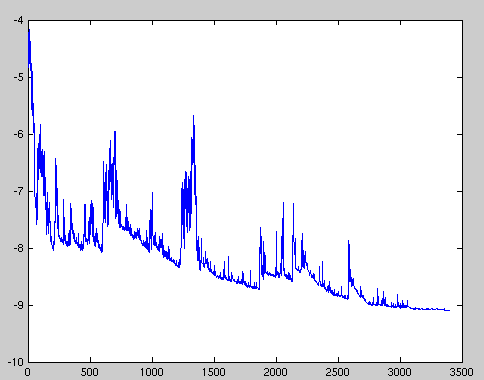
\includegraphics[height=7cm]{\calculusroot/images/sgd_fluctuation.png}
    \caption{SGD波动}
    \label{fig:sgd_fluctuation}
\end{figure}

与批梯度下降法的收敛会使得损失函数陷入局部最小相比,
由于SGD的波动性,一方面,波动性使得SGD可以跳到新的和潜在更好的局部最优;
另一方面,这使得最终收敛到特定最小值的过程变得复杂,因为SGD会一直持续波动。
然而,已经证明当我们缓慢减小学习率,SGD与批梯度下降法具有相同的收敛行为,
对于非凸优化和凸优化,可以分别收敛到局部最小值和全局最小值。
与批梯度下降的代码相比,SGD的代码片段仅仅是在对训练样本的遍历和利用每一条样本计算梯度的过程中增加一层循环。
注意在每一次循环中,最好先随机打乱训练样本。


\subsubsection{Mini-batch gradient descent}
小批量梯度下降法最终结合了上述两种方法的优点,在每次更新时使用$n$个小批量训练样本:
\[
    \theta = \theta - \eta \cdot \nabla_{\theta}{J(\theta;x^{(i:i+n)};y^{(i:i+n)})}
\]

假设训练集有$m$个样本,每个mini-batch(训练集的一个子集)有$b$个样本,
那么,整个训练集可以分成$\frac{m}{b}$个mini-batch。

这种方法,
a) 减少参数更新的方差,这样可以得到更加稳定的收敛结果;
b) 可以利用最新的深度学习库中高度优化的矩阵优化方法,高效地求解每个小批量数据的梯度。

通常,小批量数据的大小在50到256之间,也可以根据不同的应用有所变化。
当训练神经网络模型时,小批量梯度下降法是典型的选择算法,当使用小批量梯度下降法时,也将其称为SGD。


\subsection{相关优化}
虽然Vanilla小批量梯度下降法并不能保证较好的收敛性,但是需要强调的是,这也给我们留下了如下的一些挑战:
\begin{itemize}
    \item 选择一个合适的学习率可能是困难的。
          学习率太小会导致收敛的速度很慢,学习率太大会妨碍收敛,导致损失函数在最小值附近波动甚至偏离最小值。

    \item 学习率调整试图在训练的过程中通过例如退火的方法调整学习率,
          即根据预定义的策略或者当相邻两代之间的下降值小于某个阈值时减小学习率。
          然而,策略和阈值需要预先设定好,因此无法适应数据集的特点。

    \item 此外,对所有的参数更新使用同样的学习率。
          如果数据是稀疏的,同时,特征的频率差异很大时,我们也许不想以同样的学习率更新所有的参数,
          对于出现次数较少的特征,我们对其执行更大的学习率。

    \item 高度非凸误差函数普遍出现在神经网络中,在优化这类函数时,
          另一个关键的挑战是使函数避免陷入无数次优的局部最小值。
          Dauphin等人指出出现这种困难实际上并不是来自局部最小值,
          而是来自鞍点,即那些在一个维度上是递增的,而在另一个维度上是递减的。
          这些鞍点通常被具有相同误差的点包围,因为在任意维度上的梯度都近似为0,所以SGD很难从这些鞍点中逃开。
\end{itemize}

\subsubsection{Momentum}

\[
    \Delta x_{t} = \rho \Delta x_{t-1} - \eta g_{t}
\]

SGD很难通过陡谷,即在一个维度上的表面弯曲程度远大于其他维度的区域,这种情况通常出现在局部最优点附近。
在这种情况下,SGD摇摆地通过陡谷的斜坡,同时,沿着底部到局部最优点的路径上只是缓慢地前进,
这个过程如图 \ref{fig:without_momentum} 所示。

\begin{figure}[H]
    \subfigure[普通SGD]{
        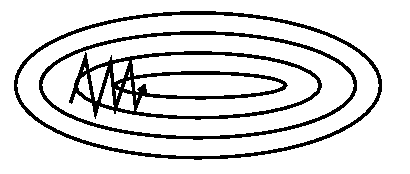
\includegraphics[scale=0.5]{\calculusroot/images/without_momentum.png}
        \label{fig:without_momentum}
    }
    \subfigure[带有冲量的SGD]{
        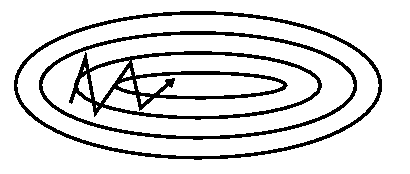
\includegraphics[scale=0.5]{\calculusroot/images/with_momentum.png}
        \label{fig:with_momentum}
    }
    \caption{效果对比图}
\end{figure}

如图 \ref{fig:with_momentum} 所示,动量法是一种帮助SGD在相关方向上加速并抑制摇摆的一种方法。
动量法将历史步长的更新向量的一个分量 $\gamma$ 增加到当前的更新向量中
\begin{align*}
    & v_t = \gamma v_{t-1} + \eta \nabla_{\theta}{J(\theta)} \\
    & \theta = \theta - v_{t}
\end{align*}
动量项 $\gamma$ 通常设置为0.9或者类似的值。

从本质上说,动量法,就像我们从山上推下一个球,球在滚下来的过程中累积动量,变得越来越快
(直到达到终极速度,如果有空气阻力的存在,则 $\gamma < 1$)。
同样的事情也发生在参数的更新过程中:对于在梯度点处具有相同的方向的维度,其动量项增大,
对于在梯度点处改变方向的维度,其动量项减小。
因此,我们可以得到更快的收敛速度,同时可以减少摇摆。


相关实验:\url{https://github.com/hsmyy/zhihuzhuanlan/blob/master/momentum.ipynb}


\subsubsection{Nesterov accelerated gradient}

\url{https://github.com/WarBean/zhihuzhuanlan/blob/master/Momentum_Nesterov.ipynb}

\begin{align*}
    & v_t = \gamma v_{t-1} + \eta \nabla_{\theta}{J(\theta - \gamma v_{t-1})} \\
    & \theta = \theta - v_{t}
\end{align*}




\subsubsection{Adagrad}

\[
    \Delta x_{t} = -\frac{\eta}{\sqrt{\sum_{\tau = 1}^{t}{g_{\tau}^2}}} g_{t}
\]



\subsubsection{RMSprop}
\href{https://arxiv.org/abs/1502.04390}{Equilibrated adaptive learning rates for non-convex optimization}

\begin{align*}
    E[g^2]_{t} = 0.9 E[g^2]_{t-1} + 0.1 g_{t}^2 \\
    \theta_{t+1} = \theta_{t} - \frac{\eta}{\sqrt{E[g^2]_{t} + \epsilon}} g_{t}
\end{align*}



\subsubsection{Adadelta}
在梯度下降法中,学习率是一个需要人为设定的超参数,通常通过人工不断的调整,从而选择效果最好的学习率。
超过这个数值,模型训练的时候无法收敛;小于这个数值,又会导致模型收敛的很慢。
在很多问题中,选择合适的学习率需要靠直觉去选择,没有科学的选择方法。

Adadelta\cite{Zeiler:2012aa} 通过在每个维度上分别引入一个动态的学习率来避免人工选择学习率时遇到的问题。

\[
    E[g^2]_t = \rho E[g^2]_{t-1} + (1 - \rho)g_{t}^2
\]

据说,Adadelta 在深层 RNN 的架构中表现的很好(需要验证)。



\subsubsection{Adam}
\subsubsection{AdaMax}
\subsubsection{Nadam}
\subsubsection{Visualization of algorithms}
\subsubsection{Which optimizer to choose?}

\subsection{Parallelizing and distributing SGD}
\subsubsection{Hogwild!}
\subsubsection{Downpour SGD}
\subsubsection{Delay-tolerant Algorithms for SGD}
\subsubsection{TensorFlow}

\subsubsection{Elastic Averaging SGD}
\subsection{Additional strategies for optimizing SGD}
\subsubsection{Shuffling and Curriculum Learning}
\subsubsection{Batch normalization}

\subsubsection{Early Stopping}
\subsubsection{Gradient noise}


\subsubsection{Online}
随着互联网行业的蓬勃发展,数据变得越来越``廉价''。很多应用有实时的,不间断的训练数据产生。在线学习(Online Learning)算法就是充分利用实时数据的一个训练算法。

Online GD与mini-batch GD/SGD的区别在于,所有训练数据只用一次,然后丢弃。这样做的好处是可以获得模型的变化趋势。比如搜索广告的点击率(CTR)预估模型,网民的点击行为会随着时间改变。用batch算法(每天更新一次)一方面耗时较长(需要对所有历史数据重新训练);另一方面,无法及时反馈用户的点击行为迁移。而Online Leaning的算法可以实时的最终网民的点击行为迁移。

\subsection{深入阅读材料}
\begin{enumerate}
    \item \href{https://arxiv.org/abs/1606.04474}{Learning to learn by gradient descent by gradient descent}



\end{enumerate}






\section{牛顿迭代法}
\subsection{基本原理}
假设 $f(x) = 0$ 为待求解方程,利用传统方法求解,牛顿法求解方程的公式:
\[
f(x_0 + \Delta x) = f(x_0) + f'(x_0)\Delta x
\]
即
\[
    f(x) = f(x_0) + f'(x_0)(x - x_0)
\]

令 $f(x) = 0$,我们能够得到迭代公式:
\[
    x = x_0 - \frac{f(x_0)}{f'(x_0)} \Rightarrow x_{n+1} = x_n - \frac{f(x_n)}{f'(x_n)}
\]
通过逐次迭代,牛顿法将逐步逼近最优值,也就是方程的解。

解决 $f(x) = 0$ 的问题,我们用了一阶泰勒展开:
\[
    f(x) = f(x_0) + f'(x_0)*(x-x_0) + o((x-x_0))
\]
去掉末位高阶展开项,代入 $x = x_0 + \Delta x$,得到:
\[
    f(x) = f(x_0 + \Delta x) = f(x_0) + f'(x_0)\Delta x
\]


那么,要解决 $f'(x) = 0$ 的问题,我们就需要二阶泰勒展开:
\[
    f(x) = f(x_0) + f'(x_0)*(x-x_0) + \frac{f''(x_0)}{2}*(x-x_0)^2 + o((x-x_0)^2)
\]
去掉末位高阶展开项,代入 $x = x_0+\Delta x$,得到:
\[
    f(x) = f(x_0+\Delta x) = f(x_0) + f'(x_0) \Delta x + \frac{f''(x_0) (\Delta x)^2}{2}
\]
求导计算: $f'(x) = f'(x_0+\Delta x) = 0$,得到:
\[
    [f(x_0) + f'(x_0)(x−x_0) + \frac{f''(x_0)(x−x_0)^2}{2}]′ = 0
\]
整理:
\begin{align*}
    & f'(x_0) + f''(x_0)(x−x_0) = 0 \\
    & x = x_0 − \frac{f'(x_0)}{f''(x_0)} \Rightarrow  x_{n+1} = x_n - \frac{f'(x_n)}{f''(x_n)}
\end{align*}

\subsection{拟牛顿条件}

\section{拟牛顿法(Quasi-Newton)}
\subsection{DFP 算法}
\subsection{BFGS算法}
\subsection{L-BFGS 算法}


\section{共轭梯度法(Conjugate Gradient)}
学习资料
\begin{enumerate}
\item《最优化理论与方法》 袁亚湘 孙文瑜
\item http://blog.csdn.net/nocml/article/details/8287466
\item Updating Quasi-Newton Matrices with Limited Storage , Jorge Nocedal
\item Nonlinear Programming, second edition, Dimitri P. Bertsekas
\item《广告数据上的大规模机器学习》  夏粉
\end{enumerate}

\ifx\mathnotes\undefined
    \bibliography{\notesroot/reference/reference.bib}
\end{document}

\fi

\chapter{线性代数}
\chapter{概率率与数理统计}
\chapter{信息论}


\part{机器学习基础}
\chapter{广义线性模型}
\chapter{朴素贝叶斯}
\ifx\mlbook\undefined
    \documentclass[10pt,a4paper]{ctexbook}
    \providecommand{\pathroot}{../..}

    \usepackage[CJKbookmarks,colorlinks,linkcolor=red]{hyperref}
    \usepackage{geometry}
    \usepackage{amsmath}
    \usepackage{CJK,CJKnumb}
    \usepackage{fontspec}
    \usepackage[table, x11names]{xcolor}
    \usepackage{array, booktabs, boldline}
    \usepackage{cellspace}
    \usepackage{float}
    \usepackage{amsfonts}
    \usepackage{color}
    \usepackage{graphicx}
    \usepackage{animate}

    \setlength\cellspacetoplimit{4pt}
    \setlength\cellspacebottomlimit{4pt}

    \geometry{left=3.0cm,right=3.0cm,top=2.5cm,bottom=2.5cm}
    \setmainfont{SimSun}
    \XeTeXlinebreaklocale "zh"
    \XeTeXlinebreakskip = 0pt plus 1pt minus 0.1pt
    \setlength{\baselineskip}{20pt}

    \title{强化学习}
    \author{Donald Cheung\\jianzhang9102@gmail.com}
    \date{Nov 11, 2017}

    \begin{document}
    \maketitle
    \tableofcontents
\fi

\chapter{强化学习}

\section{蒙特卡罗树搜索}
\href{https://www.zhihu.com/question/39916945}{蒙特卡洛树是什么算法?}


蒙特卡罗树搜索(Monte Carlo Tree Search)并不是一种"模拟人"的算法。
而是通过随机的对游戏进行推演来逐渐建立一棵不对称的搜索树的过程。
可以看成是某种意义上的强化学习,当然这一点学界还有一些争议。

蒙特卡罗树搜索大概可以被分成四步:
选择(Selection),拓展(Expansion),模拟(Simulation),反向传播(Backpropagation)。

在开始阶段,搜索树只有一个节点,也就是我们需要决策的局面。

搜索树中的每一个节点包含了三个基本信息:代表的局面,被访问的次数,累计评分。

\begin{enumerate}
\item 选择(Selection)
在选择阶段,需要从根节点,也就是要做决策的局面R出发向下选择出一个最急迫需要被拓展的节点N,局面R是是每一次迭代中第一个被检查的节点;
对于被检查的局面而言,他可能有三种可能:
    \begin{enumerate}
    \item 该节点所有可行动作都已经被拓展过
    \item 该节点有可行动作还未被拓展过
    \item 这个节点游戏已经结束了(例如已经连成五子的五子棋局面)
    \end{enumerate}

对于这三种可能:
    \begin{enumerate}
    \item 如果所有可行动作都已经被拓展过了,那么我们将使用UCB公式计算该节点所有子节点的UCB值,并找到值最大的一个子节点继续检查。反复向下迭代。
    \item 如果被检查的局面依然存在没有被拓展的子节点(例如说某节点有20个可行动作,但是在搜索树中才创建了19个子节点),那么我们认为这个节点就是本次迭代的的目标节点N,并找出N还未被拓展的动作A。执行步骤[2]
    \item 如果被检查到的节点是一个游戏已经结束的节点。那么从该节点直接执行步骤[4]。
    \end{enumerate}
每一个被检查的节点的被访问次数在这个阶段都会自增。在反复的迭代之后,我们将在搜索树的底端找到一个节点,来继续后面的步骤。

\item 拓展(Expansion)
在选择阶段结束时候,我们查找到了一个最迫切被拓展的节点N,以及他一个尚未拓展的动作A。在搜索树中创建一个新的节点Nn作为N的一个新子节点。Nn的局面就是节点N在执行了动作A之后的局面。

\item 模拟(Simulation)为了让Nn得到一个初始的评分。我们从Nn开始,让游戏随机进行,直到得到一个游戏结局,这个结局将作为Nn的初始评分。一般使用胜利/失败来作为评分,只有1或者0。

\item 反向传播(Backpropagation)
在Nn的模拟结束之后,它的父节点N以及从根节点到N的路径上的所有节点都会根据本次模拟的结果来添加自己的累计评分。如果在[1]的选择中直接发现了一个游戏结局的话,根据该结局来更新评分。每一次迭代都会拓展搜索树,随着迭代次数的增加,搜索树的规模也不断增加。当到了一定的迭代次数或者时间之后结束,选择根节点下最好的子节点作为本次决策的结果。一次迭代的图例
\begin{figure}[ht]
    \centering
    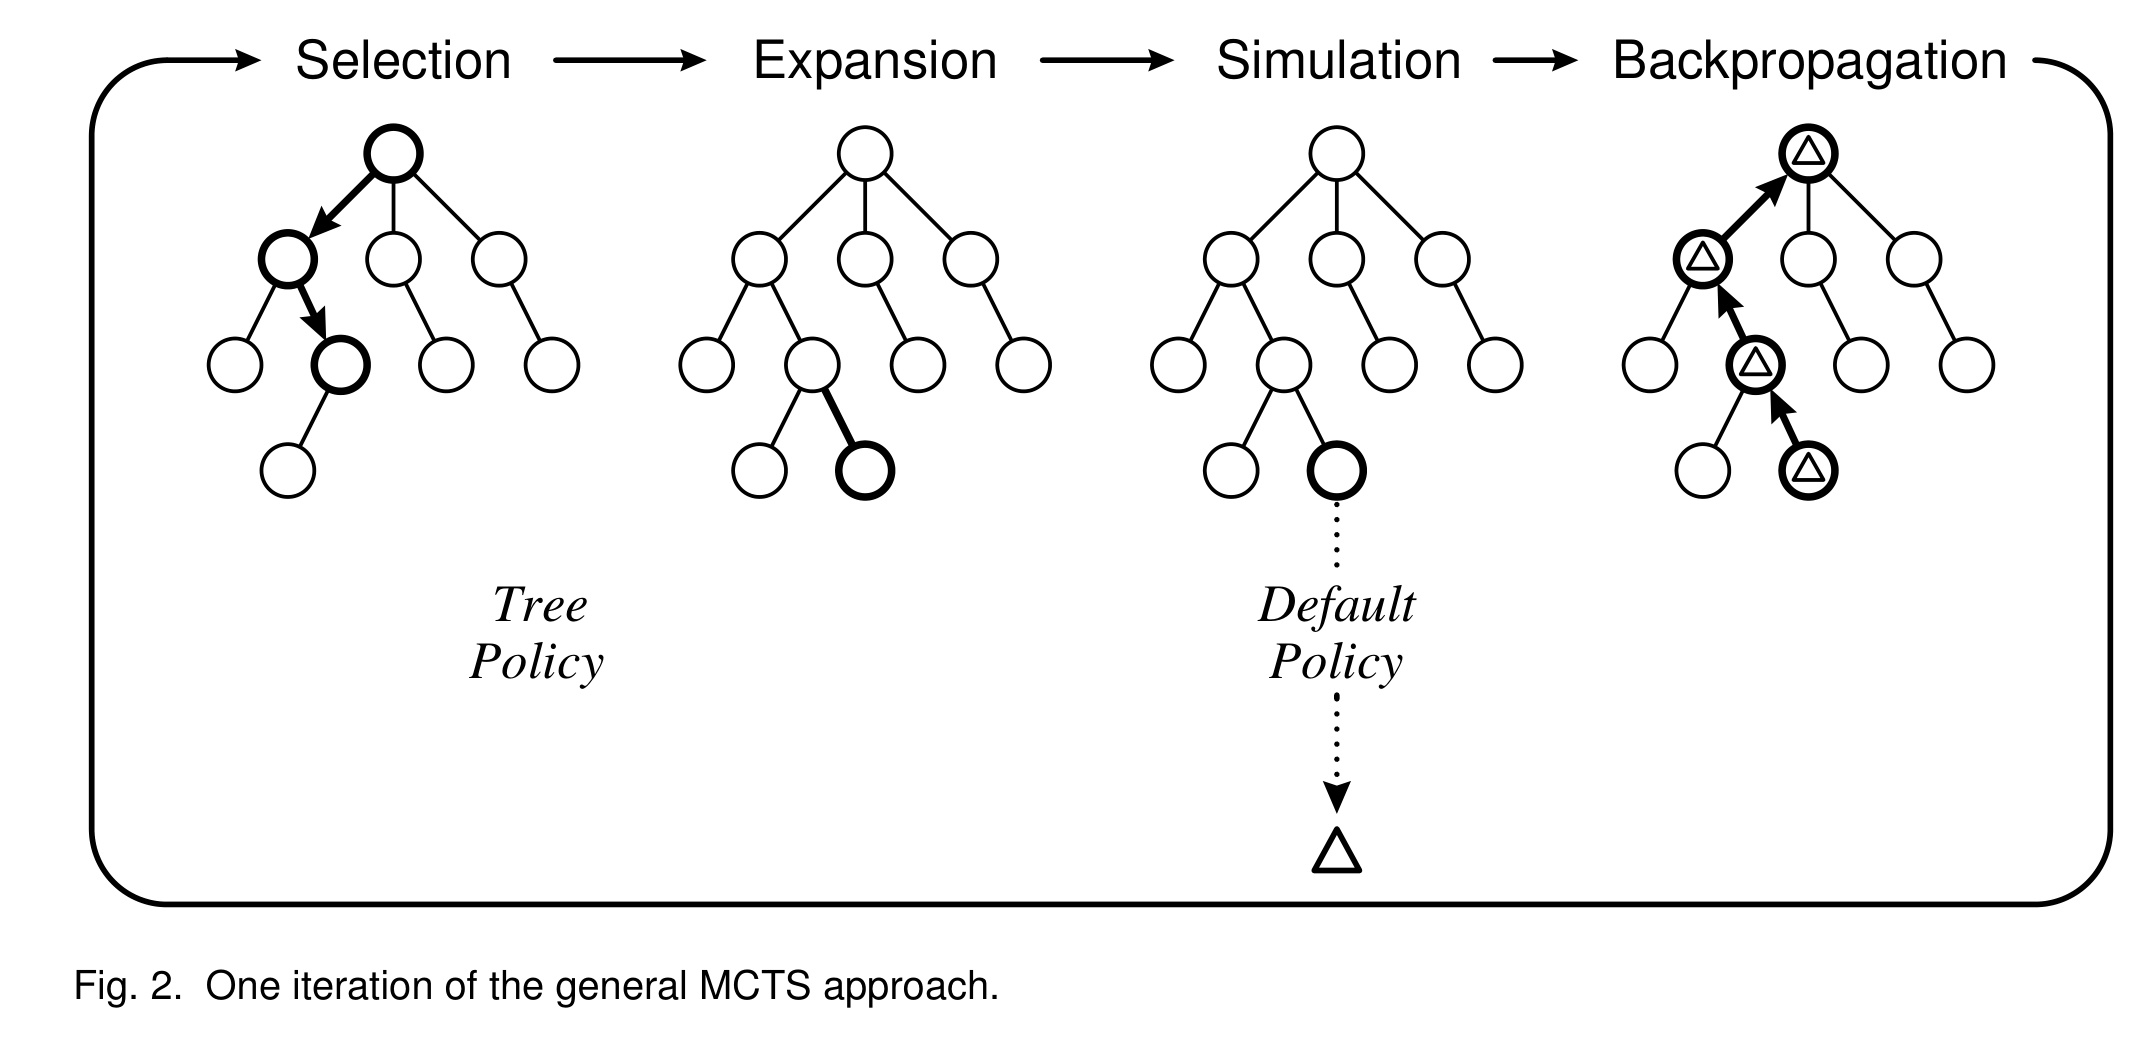
\includegraphics[height=7cm]{\pathroot/theory/reinforcement_learning/images/mcts_approach.jpg}
    \label{fig:mcts_approach}
\end{figure}



\end{enumerate}

上面描述的是UCT (UCB for Tree)算法,可以说是最经典的蒙特卡罗树搜索算法了。
但随着算法的发展,MCTS已经有了非常大的改变。
例如很多围棋AI都已经不再使用纯粹的UCB公式而改用效果更好的UCB1-Tuned了,而搜索方法上也有了非常多的改动了。

Reference:
\begin{itemize}
\item Browne C B, Powley E, Whitehouse D, et al. A Survey of Monte Carlo Tree Search Methods[J]. IEEE Transactions on Computational Intelligence \& Ai in Games, 2012, 4:1(1):1-43.
\item P. Auer, N. Cesa-Bianchi, and P. Fischer, “Finite-time Analysis  of the Multiarmed Bandit Problem,” Mach. Learn., vol. 47, no. 2,  pp. 235-256, 2002.
\end{itemize}

\ifx\mlbook\undefined
    \end{document}
\fi



\part{神经网络}
\chapter{前馈神经网络}
\chapter{RNN}
\chapter{CNN}
\chapter{RBM}
\ifx\mlbook\undefined
    \documentclass[10pt,a4paper]{ctexbook}
    \providecommand{\pathroot}{../..}

    \usepackage[CJKbookmarks,colorlinks,linkcolor=red]{hyperref}
    \usepackage{geometry}
    \usepackage{amsmath}

    \geometry{left=3.0cm,right=3.0cm,top=2.5cm,bottom=2.5cm}
    \setmainfont{SimSun}
    \XeTeXlinebreaklocale "zh"
    \XeTeXlinebreakskip = 0pt plus 1pt minus 0.1pt

    \begin{document}
    \setlength{\baselineskip}{20pt}
    \title{Logistic回归}
    \author{Donald Cheung\\jianzhang9102@gmail.com}
    \date{Sep 8, 2017}
    \maketitle
    \tableofcontents
\fi

\chapter{神经网络}
\section{前馈神经网络}
Backpropagation Algorithm(BP算法)
\href{https://machinelearningmastery.com/implement-backpropagation-algorithm-scratch-python/}{How to Implement the Backpropagation Algorithm From Scratch In Python}

\section{RNN}
RNN理论基础,包括历史、类别、训练算法等。
\href{https://github.com/szcom/rnnlib}{rnnlib}



\subsection{BPTT}
\href{http://proceedings.mlr.press/v28/pascanu13.pdf}{On the difficulty of training recurrent neural networks}

\href{https://arxiv.org/abs/1211.5063}{On the difficulty of training recurrent neural networks}

\href{https://arxiv.org/abs/1606.03401}{Memory-Efficient Backpropagation Through Time}

\href{http://axon.cs.byu.edu/~martinez/classes/678/Papers/Werbos_BPTT.pdf}{Backpropagation Through Time: What It Does and How to Do It}

\href{https://arxiv.org/pdf/1406.1078v3.pdf}{Learning Phrase Representations using RNN Encoder-Decoder for Statistical Machine Translation}

\href{http://www.cs.utoronto.ca/~ilya/pubs/ilya_sutskever_phd_thesis.pdf}{Ilya Sutskever, Training Recurrent Neural Networks, Thesis, 2013}

\href{https://arxiv.org/abs/1503.04069}{LSTM: A Search Space Odyssey}

\href{https://arxiv.org/abs/1506.00019}{A Critical Review of Recurrent Neural Networks for Sequence Learning}

\href{https://jramapuram.github.io/ramblings/rnn-backrpop/}{BLOG: RNN Backprop Through Time Equations}

vanilla RNNs trained with BPTT \href{http://www.jmlr.org/proceedings/papers/v28/pascanu13.pdf}{have difficulties} learning long-term dependencies (e.g. dependencies between steps that are far apart) due to what is called the vanishing/exploding gradient problem. There exists some machinery to deal with these problems, and certain types of RNNs (like LSTMs) were specifically designed to get around them.

\[
\begin{aligned}
C_{i,j} & = -\tilde{P_{ij}} * o_{i,j} + log(1 + e^{o_{i,j}})\\o_{i,j} & = o_i - o_j\\\tilde{P_{i,j}} & = \{0, 0.5, 1\} \ or \ \{0, 1\}
\end{aligned}
\]

Cosine Similarity Layer. The cosine similarity equation is here.
\[similarity = cos(\theta) = {\mathbf{a} \cdot \mathbf{b} \over \|\mathbf{a}\| \|\mathbf{b}\|}\]
The size of a is M, size of b is M*N, Similarity will be calculated N times by step M. The output size is N. The scale will be multiplied to similarity.

Note that the above computation is for one sample. Multiple samples are processed in one batch.

\begin{table}[H]
\centering
\begin{tabular}{|l|l|l|}
\hline
Neural Layer & Description & Index variable\\
\hline
$x(t)$ & input layer & $i$ \\
$s(t-1)$ & previous hidden (state) layer & $h$ \\
$s(t)$ & hidden (state) layer & $j$ \\
$y(t)$ & output layer & $k$ \\
\hline
\end{tabular}%
\caption{Notations in the recurrent neural network.}
\label{tab:rnn-notations}
\end{table}

\inputminted{python}{reference/code/bptt.py}

\begin{minted}[mathescape,
               linenos,
               numbersep=5pt,
               gobble=2,
               frame=lines,
               framesep=2mm]{csharp}
  string title = "This is a Unicode πin the sky";
  /*  
  Defined as $\pi=\lim_{n\to\infty}\frac{P_n}{d}$ where $P$ is the perimeter
  of an $n$-sided regular polygon circumscribing a
  circle of diameter $d$.
  */  
  const double pi = 3.1415926535
\end{minted}


\begin{itemize}
\item Hochreiter S, Schmidhuber J. \href{http://web.eecs.utk.edu/~itamar/courses/ECE-692/Bobby_paper1.pdf}{Long short-term memory[J]}. Neural computation, 1997, 9(8): 1735-1780.
\item Bengio Y, Simard P, Frasconi P. \href{http://www-dsi.ing.unifi.it/~paolo/ps/tnn-94-gradient.pdf}{Learning long-term dependencies with gradient descent is difficult[J]}. IEEE transactions on neural networks, 1994, 5(2): 157-166.
\item \href{https://arxiv.org/pdf/1610.09038.pdf}{Professor Forcing: A New Algorithm for Training Recurrent Networks}
\item \href{http://ir.hit.edu.cn/~jguo/docs/notes/bptt.pdf}{BackPropagation Through Time}
\item \href{http://nn.cs.utexas.edu/downloads/papers/james.sardnet.pdf}{SARDNET: A Self-Organizing Feature Map for Sequences*}
\item \href{http://colah.github.io/posts/2015-08-Understanding-LSTMs/}{Understanding LSTMs}
\end{itemize}

\begin{itemize}
\item $x_t$是时刻$t$的输入。例如,$x_1$可以是一个one-hot的稀疏向量,表示一个句子中的第二个单词。
\item $s_t$是时刻$t$的隐层状态,是网络的记忆单元。$s_t$的计算依赖于当前时刻的输入以及之前的隐层状态值:$s_t=f(Ux_t+Ws_{t-1})$。函数$f$通常是非线性函数,例如$tanh$或者是$ReLU$。
\item $o_t$是时刻$t$的输出。例如,当我们需要预测一个句子中的下一个词时,$o_t$为词典中每个词的概率,也即$o_t=softmax(Vs_t)$
\item 需要注意的是,RNN中的$U,V,W$参数是共享的。
\end{itemize}



\section{CNN}

\section{常用激活函数}

\subsection{sigmoid}
\subsection{softmax}
\subsection{tanh}
\subsection{ReLU}

\section{常用损失函数}
\subsection{交叉熵}

$L(y,o)=-\frac{1}{N}\sum\limits_{n \in N}{y_{n}\log{o_{n}}}$

\section{RNN技术综述}

\subsection{A Critical Review of Recurrent Neural Networks for Sequence Learning}

\subsection{Neural Turing Machines}
\href{Neural Turing Machines}{https://arxiv.org/abs/1410.5401}

\subsection{Attention}
\href{https://distill.pub/2016/augmented-rnns/}{Attention and Augmented Recurrent Neural Networks}

\href{https://arxiv.org/abs/1706.03762}{Attention Is All You Need}

\subsubsection{Soft Attention}
The concept of attention is the most interesting recent architectural innovation in neural networks.

\subsubsection{Hard Attention}
\href{Inferring Algorithmic Patterns with Stack-Augmented Recurrent Nets}{https://arxiv.org/abs/1503.01007}
\href{Reinforcement Learning Neural Turing Machines - Revised}{https://arxiv.org/abs/1505.00521}
\href{Show, Attend and Tell: Neural Image Caption Generation with Visual Attention}{https://arxiv.org/abs/1502.03044}

\section{People}
\href{Alex Graves}{http://www.cs.toronto.edu/~graves/}
\href{Ilya Sutskever}{http://www.cs.toronto.edu/~ilya/}
\href{Tomas Mikolov}{http://www.rnnlm.org/}

\subsection{Reinforcement Learning}
\href{David Silver}{http://www0.cs.ucl.ac.uk/staff/d.silver/web/Home.html}
\href{Pieter Abbeel}{https://people.eecs.berkeley.edu/~pabbeel/}


\section{文本分类}
\subsection{相关论文}

\begin{itemize}
\item \href{http://www.aclweb.org/old_anthology/D/D15/D15-1167.pdf}{Document Modeling with Gated Recurrent Neural Network for Sentiment Classification}
\item \href{http://www.aclweb.org/anthology/N16-1174}{Hierarchical Attention Networks for Document Classification}
\item \href{http://www.aclweb.org/anthology/P15-1109}{End-to-end Learning of Semantic Role Labeling Using Recurrent Neural Networks}
\end{itemize}

\subsubsection{\href{https://arxiv.org/abs/1408.5882}{Convolutional Neural Networks for Sentence Classification}}

相关资料:
\begin{itemize}
\item 论文代码:\url{https://github.com/yoonkim/CNN_sentence}
\item 代码: \url{https://github.com/dennybritz/cnn-text-classification-tf}
\item \href{http://www.wildml.com/2015/12/implementing-a-cnn-for-text-classification-in-tensorflow/}{Implementing a CNN for Text Classification in TensorFlow}
\item \href{http://www.wildml.com/2015/11/understanding-convolutional-neural-networks-for-nlp/}{Understanding Convolutional Neural Networks for NLP}
\end{itemize}

\subsubsection{\href{https://arxiv.org/abs/1510.03820}{A Sensitivity Analysis of (and Practitioners’ Guide to) Convolutional Neural Networks for Sentence Classification}}

\subsubsection{Convolutional Neural Networks applied to NLP}

The most natural fit for CNNs seem to be classifications tasks, such as Sentiment Analysis, Spam Detection or Topic Categorization. Convolutions and pooling operations lose information about the local order of words, so that sequence tagging as in PoS Tagging or Entity Extraction is a bit harder to fit into a pure CNN architecture (though not impossible, you can add positional features to the input).

[1] Evaluates a CNN architecture on various classification datasets, mostly comprised of Sentiment Analysis and Topic Categorization tasks. The CNN architecture achieves very good performance across datasets, and new state-of-the-art on a few. Surprisingly, the network used in this paper is quite simple, and that's what makes it powerful. The input layer is a sentence comprised of concatenated word2vec word embeddings. That's followed by a convolutional layer with multiple filters, then a max-pooling layer, and finally a softmax classifier. The paper also experiments with two different channels in the form of static and dynamic word embeddings, where one channel is adjusted during training and the other isn't. A similar, but somewhat more complex, architecture was previously proposed in [2]. [6] Adds an additional layer that performs "semantic clustering" to this network architecture.

[4] Trains a CNN from scratch, without the need for for pre-trained word vectors like word2vec or GloVe. It applies convolutions directly to one-hot vectors. The author also proposes a space-efficient bag-of-words-like representation for the input data, reducing the number of parameters the network needs to learn. In [5] the author extends the model with an additional unsupervised "region embedding" that is learned using a CNN predicting the context of text regions. The approach in these papers seems to work well for long-form texts (like movie reviews), but their performance on short texts (like tweets) isn't clear. Intuitively, it makes sense that using pre-trained word embeddings for short texts would yield larger gains than using them for long texts.

Building a CNN architecture means that there are many hyperparameters to choose from, some of which I presented above: Input represenations (word2vec, GloVe, one-hot), number and sizes of convolution filters, pooling strategies (max, average), and activation functions (ReLU, tanh). [7] performs an empirical evaluation on the effect of varying hyperparameters in CNN architectures, investigating their impact on performance and variance over multiple runs. If you are looking to implement your own CNN for text classification, using the results of this paper as a starting point would be an excellent idea. A few results that stand out are that max-pooling always beat average pooling, that the ideal filter sizes are important but task-dependent, and that regularization doesn't seem to make a big different in the NLP tasks that were considered. A caveat of this research is that all the datasets were quite similar in terms of their document length, so the same guidelines may not apply to data that looks considerably different.

[8] explores CNNs for Relation Extraction and Relation Classification tasks. In addition to the word vectors, the authors use the relative positions of words to the entities of interest as an input to the convolutional layer. This models assumes that the positions of the entities are given, and that each example input contains one relation. [9] and [10] have explored similar models.

Another interesting use case of CNNs in NLP can be found in [11] and [12], coming out of Microsoft Research. These papers describe how to learn semantically meaningful representations of sentences that can be used for Information Retrieval. The example given in the papers includes recommending potentially interesting documents to users based on what they are currently reading. The sentence representations are trained based on search engine log data.

Most CNN architectures learn embeddings (low-dimensional representations) for words and sentences in one way or another as part of their training procedure. Not all papers though focus on this aspect of training or investigate how meaningful the learned embeddings are. [13] presents a CNN architecture to predict hashtags for Facebook posts, while at the same time generating meaningful embeddings for words and sentences. These learned embeddings are then successfully applied to another task – recommending potentially interesting documents to users, trained based on clickstream data.

Character-Level CNNs

So far, all of the models presented were based on words. But there has also been research in applying CNNs directly to characters. [14] learns character-level embeddings, joins them with pre-trained word embeddings, and uses a CNN for Part of Speech tagging. [15][16] explores the use of CNNs to learn directly from characters, without the need for any pre-trained embeddings. Notably, the authors use a relatively deep network with a total of 9 layers, and apply it to Sentiment Analysis and Text Categorization tasks. Results show that learning directly from character-level input works very well on large datasets (millions of examples), but underperforms simpler models on smaller datasets (hundreds of thousands of examples). [17] explores to application of character-level convolutions to Language Modeling, using the output of the character-level CNN as the input to an LSTM at each time step. The same model is applied to various languages.

What's amazing is that essentially all of the papers above were published in the past 1-2 years. Obviously there has been excellent work with CNNs on NLP before, as in Natural Language Processing (almost) from Scratch, but the pace of new results and state of the art systems being published is clearly accelerating.

\begin{itemize}
\item Kim, Y. (2014). \href{http://arxiv.org/pdf/1408.5882}{Convolutional Neural Networks for Sentence Classification}. Proceedings of the 2014 Conference on Empirical Methods in Natural Language Processing (EMNLP 2014), 1746–1751.
\item Kalchbrenner, N., Grefenstette, E., \& Blunsom, P. (2014). \href{http://arxiv.org/pdf/1404.2188.pdf}{A Convolutional Neural Network for Modelling Sentences}. Acl, 655–665.
\item Yann N. Dauphin, et al. \href{https://arxiv.org/pdf/1612.08083v1.pdf}{Language Modeling with Gated Convolutional Networks[J]} arXiv preprint arXiv:1612.08083, 2016.
\end{itemize}

%[3] Santos, C. N. dos, & Gatti, M. (2014). Deep Convolutional Neural Networks for Sentiment Analysis of Short Texts. In COLING-2014 (pp. 69–78).
%[4] Johnson, R., & Zhang, T. (2015). Effective Use of Word Order for Text Categorization with Convolutional Neural Networks. To Appear: NAACL-2015, (2011).
%[5] Johnson, R., & Zhang, T. (2015). Semi-supervised Convolutional Neural Networks for Text Categorization via Region Embedding.
%[6] Wang, P., Xu, J., Xu, B., Liu, C., Zhang, H., Wang, F., & Hao, H. (2015). Semantic Clustering and Convolutional Neural Network for Short Text Categorization. Proceedings ACL 2015, 352–357.
%[7] Zhang, Y., & Wallace, B. (2015). A Sensitivity Analysis of (and Practitioners’ Guide to) Convolutional Neural Networks for Sentence Classification,
%[8] Nguyen, T. H., & Grishman, R. (2015). Relation Extraction: Perspective from Convolutional Neural Networks. Workshop on Vector Modeling for NLP, 39–48.
%[9] Sun, Y., Lin, L., Tang, D., Yang, N., Ji, Z., & Wang, X. (2015). Modeling Mention , Context and Entity with Neural Networks for Entity Disambiguation, (Ijcai), 1333–1339.
%[10] Zeng, D., Liu, K., Lai, S., Zhou, G., & Zhao, J. (2014). Relation Classification via Convolutional Deep Neural Network. Coling, (2011), 2335–2344. 
%[11] Gao, J., Pantel, P., Gamon, M., He, X., & Deng, L. (2014). Modeling Interestingness with Deep Neural Networks.
%[12] Shen, Y., He, X., Gao, J., Deng, L., & Mesnil, G. (2014). A Latent Semantic Model with Convolutional-Pooling Structure for Information Retrieval. Proceedings of the 23rd ACM International Conference on Conference on Information and Knowledge Management – CIKM ’14, 101–110. 
%[13] Weston, J., & Adams, K. (2014). # T AG S PACE : Semantic Embeddings from Hashtags, 1822–1827.
%[14] Santos, C., & Zadrozny, B. (2014). Learning Character-level Representations for Part-of-Speech Tagging. Proceedings of the 31st International Conference on Machine Learning, ICML-14(2011), 1818–1826. 
%[15] Zhang, X., Zhao, J., & LeCun, Y. (2015). Character-level Convolutional Networks for Text Classification, 1–9.
%[16] Zhang, X., & LeCun, Y. (2015). Text Understanding from Scratch. arXiv E-Prints, 3, 011102.
%[17] Kim, Y., Jernite, Y., Sontag, D., & Rush, A. M. (2015). Character-Aware Neural Language Models.

\section{RNN应用}

\subsection{Language Modeling and Generating Text}
Given a sequence of words we want to predict the probability of each word given the previous words. Language Models allow us to measure how likely a sentence is, which is an important input for Machine Translation (since high-probability sentences are typically correct). A side-effect of being able to predict the next word is that we get a generative model, which allows us to generate new text by sampling from the output probabilities. And depending on what our training data is we can generate all kinds of stuff. In Language Modeling our input is typically a sequence of words (encoded as one-hot vectors for example), and our output is the sequence of predicted words. When training the network we set $o_{t} = x_{t+1}$ since we want the output at step $t$ to be the actual next word.

Research papers about Language Modeling and Generating Text:
\begin{itemize}
\item \href{http://www.fit.vutbr.cz/research/groups/speech/publi/2010/mikolov_interspeech2010_IS100722.pdf}{Recurrent neural network based language model}
\item \href{http://www.fit.vutbr.cz/research/groups/speech/publi/2011/mikolov_icassp2011_5528.pdf}{Extensions of Recurrent neural network based language model}
\item \href{http://machinelearning.wustl.edu/mlpapers/paper_files/ICML2011Sutskever_524.pdf}{Generating Text with Recurrent Neural Networks}
\end{itemize}


Our goal is to build a Language Model using a Recurrent Neural Network. Here's what that means. Let's say we have sentence of $m$ words. A language model allows us to predict the probability of observing the sentence (in a given dataset) as:
\[
P(w_{1}, ..., w_{m})=\prod_{i=1}^{m}{P(w_{i}|w_{1},...,w_{i-1})}
\]

In words, the probability of a sentence is the product of probabilities of each word given the words that came before it. So, the probability of the sentence "He went to buy some chocolate" would be the probability of "chocolate" given "He went to buy some", multiplied by the probability of "some" given "He went to buy", and so on.

Why is that useful? Why would we want to assign a probability to observing a sentence?

First, such a model can be used as a scoring mechanism. For example, a Machine Translation system typically generates multiple candidates for an input sentence. You could use a language model to pick the most probable sentence. Intuitively, the most probable sentence is likely to be grammatically correct. Similar scoring happens in speech recognition systems.

But solving the Language Modeling problem also has a cool side effect. Because we can predict the probability of a word given the preceding words, we are able to generate new text. It's a generative model. Given an existing sequence of words we sample a next word from the predicted probabilities, and repeat the process until we have a full sentence. Andrej Karparthy \href{http://karpathy.github.io/2015/05/21/rnn-effectiveness/}{has a great post} that demonstrates what language models are capable of. His models are trained on single characters as opposed to full words, and can generate anything from Shakespeare to Linux Code.

Note that in the above equation the probability of each word is conditioned on all previous words. In practice, many models have a hard time representing such long-term dependencies due to computational or memory constraints. They are typically limited to looking at only a few of the previous words. RNNs can, in theory, capture such long-term dependencies, but in practice it's a bit more complex. We'll explore that in a later post.

一个语言模型的训练和预处理过程:

step 1. 分词、标点符号等的处理。例如英文标点符号,中文分词等。

step 2. 删除低频词。对于没有在字典里面出现的词,可以用字典里面一个特殊的词(例如UNK)来替代。在预测的时候,就有两种做法:一是将预测为UNK的词,随机用一个没有出现在字典中的词替代;另一个做法是生成句子,直到句子中没有出现UNK的词。

step 3. 增加特殊的开始和截止字符,例如<start>和<end>。这样在预测的时候,给定<start>预测下一个词,就可以完整的生成一个全新的句子了。

step 4. 生成训练数据。训练数据是把原文的词转换为ID,每个词对应一个ID号,每个ID号也对应一个词。每次预测时,都是基于当前词去预测下一个词。


\textbf{一个简单的RNN算法的计算量分析}。对于一个简单的RNN来说,有
\[
\begin{aligned}
	s_{t}=tanh(Ux_{t}+Ws_{t-1}) \\
	o_{t}=softmax(Vs_{t})
\end{aligned}
\]

假设选取字典大小为$\mathnormal{C}=8000$,隐藏层大小$H=100$。则我们有
\begin{gather*} 
x_{t} \in \mathbb{R}^{8000} \\
o_{t} \in \mathbb{R}^{8000} \\
s_{t} \in \mathbb{R}^{100} \\
U \in \mathbb{R}^{100 \times 8000} \\
V \in \mathbb{R}^{8000 \times 100} \\
W \in \mathbb{R}^{100 \times 100}
\end{gather*}

This is valuable information. Remember that $U$,$V$ and $W$ are the parameters of our network we want to learn from data. Thus, we need to learn a total of $2HC + H^{2}$ parameters. In the case of $C=8000$ and $H=100$ that's 1,610,000. The dimensions also tell us the bottleneck of our model. Note that because $x_{t}$ is a one-hot vector, multiplying it with U is essentially the same as selecting a column of U, so we don't need to perform the full multiplication. Then, the biggest matrix multiplication in our network is $Vs_{t}$. That's why we want to keep our vocabulary size small if possible.


\textbf{RNN实现}

\href{http://www.wildml.com/2015/09/recurrent-neural-networks-tutorial-part-1-introduction-to-rnns/}{Recurrent Neural Networks Tutorial, Part 1 – Introduction to RNNs}

\subsubsection{Initialization}
We start by declaring a RNN class an initializing our parameters. I'm calling this class RNNNumpy because we will implement a Theano version later. Initializing the parameters $U$,$V$ and $W$ is a bit tricky. We can't just initialize them to 0's because that would result in symmetric calculations in all our layers. We must initialize them randomly. Because proper initialization seems to have an impact on training results there has been lot of research in this area. It turns out that the best initialization depends on the activation function ($\tanh$ in our case) and one recommended approach is to initialize the weights randomly in the interval from $\left[-\frac{1}{\sqrt{n}}, \frac{1}{\sqrt{n}}\right]$ where n is the number of incoming connections from the previous layer. This may sound overly complicated, but don't worry too much it. As long as you initialize your parameters to small random values it typically works out fine.

\begin{minted}[breaklines,tabsize=2,linenos]{python}
class RNNNumpy(object):
    def __init__(self, word_dim, hidden_dim=100, bptt_truncate=4):
        # Assign instance variables
        self.word_dim = word_dim
        self.hidden_dim = hidden_dim
        self.bptt_truncate = bptt_truncate
        # Randomly initialize the network parameters
        self.U = np.random.uniform(-np.sqrt(1./word_dim), np.sqrt(1./word_dim),
                                    (hidden_dim, word_dim))
        self.V = np.random.uniform(-np.sqrt(1./hidden_dim),np.sqrt(1./hidden_dim),
                                    (word_dim, hidden_dim))
        self.W = np.random.uniform(-np.sqrt(1./hidden_dim), np.sqrt(1./hidden_dim),
                                    (hidden_dim, hidden_dim))
\end{minted}
Above, word\_dim is the size of our vocabulary, and hidden\_dim is the size of our hidden layer (we can pick it). Don't worry about the bptt\_truncate parameter for now, we'll explain what that is later.

\subsubsection{Forward Propagation}
Next, let's implement the forward propagation (predicting word probabilities) defined by our equations above:

\begin{minted}[breaklines,tabsize=2,linenos]{python}
def forward_propagation(self, x):
    # The total number of time steps
    T = len(x)
    # During forward propagation we save all hidden states in s because need them later.
    # We add one additional element for the initial hidden, which we set to 0
    s = np.zeros((T + 1, self.hidden_dim))
    s[-1] = np.zeros(self.hidden_dim)
    # The outputs at each time step. Again, we save them for later.
    o = np.zeros((T, self.word_dim))
    # For each time step...
    for t in np.arange(T):
        # Note that we are indxing U by x[t].
        #This is the same as multiplying U with a one-hot vector.
        s[t] = np.tanh(self.U[:,x[t]] + self.W.dot(s[t-1]))
        o[t] = softmax(self.V.dot(s[t]))
    return [o, s]
 
RNNNumpy.forward_propagation = forward_propagation
\end{minted}

We not only return the calculated outputs, but also the hidden states. We will use them later to calculate the gradients, and by returning them here we avoid duplicate computation. Each o\_t is a vector of probabilities representing the words in our vocabulary, but sometimes, for example when evaluating our model, all we want is the next word with the highest probability. We call this function predict:

\begin{minted}[breaklines,tabsize=2,linenos]{python}
def predict(self, x):
    # Perform forward propagation and return index of the highest score
    o, s = self.forward_propagation(x)
    return np.argmax(o, axis=1)

    RNNNumpy.predict = predict
\end{minted}


\subsubsection{Calculating the Loss}
To train our network we need a way to measure the errors it makes. We call this the loss function $L$, and our goal is find the parameters $U$,$V$ and $W$ that minimize the loss function for our training data. A common choice for the loss function is the cross-entropy loss. If we have $N$ training examples (words in our text) and C classes (the size of our vocabulary) then the loss with respect to our predictions o and the true labels y is given by:

\[
\begin{aligned}
    L(y,o) = - \frac{1}{N} \sum_{n \in N} y_{n} \log o_{n}
\end{aligned}  
\]

The formula looks a bit complicated, but all it really does is sum over our training examples and add to the loss based on how off our prediction are. The further away $y$ (the correct words) and $o$ (our predictions), the greater the loss will be. We implement the function calculate\_loss:

\begin{minted}[breaklines,tabsize=2,linenos]{python}
def calculate_total_loss(self, x, y):
    L = 0
    # For each sentence...
    for i in np.arange(len(y)):
        o, s = self.forward_propagation(x[i])
        # We only care about our prediction of the "correct" words
        correct_word_predictions = o[np.arange(len(y[i])), y[i]]
        # Add to the loss based on how off we were
        L += -1 * np.sum(np.log(correct_word_predictions))
    return L
 
def calculate_loss(self, x, y):
    # Divide the total loss by the number of training examples
    N = np.sum((len(y_i) for y_i in y))
    return self.calculate_total_loss(x,y)/N
 
RNNNumpy.calculate_total_loss = calculate_total_loss
RNNNumpy.calculate_loss = calculate_loss
\end{minted}

Let's take a step back and think about what the loss should be for random predictions. That will give us a baseline and make sure our implementation is correct. We have $C$ words in our vocabulary, so each word should be (on average) predicted with probability $\frac{1}{C}$, which would yield a loss of $L = -\frac{1}{N} N \log\frac{1}{C} = \log C$:

\begin{minted}[breaklines,tabsize=2,linenos]{python}
# Limit to 1000 examples to save time
print "Expected Loss for random predictions: %f" % np.log(vocabulary_size)
print "Actual loss: %f" % model.calculate_loss(X_train[:1000], y_train[:1000])

Expected Loss for random predictions: 8.987197
Actual loss: 8.987440
\end{minted}

Pretty close! Keep in mind that evaluating the loss on the full dataset is an expensive operation and can take hours if you have a lot of data!

\subsubsection{Training the RNN with SGD and Backpropagation Through Time (BPTT)}
Remember that we want to find the parameters $U$,$V$ and $W$ that minimize the total loss on the training data. The most common way to do this is SGD, Stochastic Gradient Descent. The idea behind SGD is pretty simple. We iterate over all our training examples and during each iteration we nudge the parameters into a direction that reduces the error. These directions are given by the gradients on the loss: $\frac{\partial L}{\partial U}$, $\frac{\partial L}{\partial V}$, $\frac{\partial L}{\partial W}$. SGD also needs a learning rate, which defines how big of a step we want to make in each iteration. SGD is the most popular optimization method not only for Neural Networks, but also for many other Machine Learning algorithms. As such there has been a lot of research on how to optimize SGD using batching, parallelism and adaptive learning rates. Even though the basic idea is simple, implementing SGD in a really efficient way can become very complex. If you want to learn more about SGD \href{http://cs231n.github.io/optimization-1/}{this} is a good place to start. Due to its popularity there are a wealth of tutorials floating around the web, and I don't want to duplicate them here. I'll implement a simple version of SGD that should be understandable even without a background in optimization.

But how do we calculate those gradients we mentioned above? In a \href{http://www.wildml.com/2015/09/implementing-a-neural-network-from-scratch/}{traditional Neural Network} we do this through the backpropagation algorithm. In RNNs we use a slightly modified version of the this algorithm called \emph{Backpropagation Through Time (BPTT)}. Because the parameters are shared by all time steps in the network, the gradient at each output depends not only on the calculations of the current time step, but also the previous time steps. If you know calculus, it really is just applying the chain rule. The next part of the tutorial will be all about BPTT, so I won't go into detailed derivation here. For a general introduction to backpropagation check out \href{http://colah.github.io/posts/2015-08-Backprop/}{this} and this \href{http://cs231n.github.io/optimization-2/}{post}. For now you can treat \textbf{BPTT} as a black box. It takes as input a training example $(x,y)$ and returns the gradients $\frac{\partial L}{\partial U}$, $\frac{\partial L}{\partial V}$, $\frac{\partial L}{\partial W}$.

\begin{minted}[breaklines,tabsize=2,linenos]{python}
def bptt(self, x, y):
    T = len(y)
    # Perform forward propagation
    o, s = self.forward_propagation(x)
    # We accumulate the gradients in these variables
    dLdU = np.zeros(self.U.shape)
    dLdV = np.zeros(self.V.shape)
    dLdW = np.zeros(self.W.shape)
    delta_o = o
    delta_o[np.arange(len(y)), y] -= 1.
    # For each output backwards...
    for t in np.arange(T)[::-1]:
        dLdV += np.outer(delta_o[t], s[t].T)
        # Initial delta calculation
        delta_t = self.V.T.dot(delta_o[t]) * (1 - (s[t] ** 2))
        # Backpropagation through time (for at most self.bptt_truncate steps)
        for bptt_step in np.arange(max(0, t-self.bptt_truncate), t+1)[::-1]:
            # print "Backpropagation step t=%d bptt step=%d " % (t, bptt_step)
            dLdW += np.outer(delta_t, s[bptt_step-1])              
            dLdU[:,x[bptt_step]] += delta_t
            # Update delta for next step
            delta_t = self.W.T.dot(delta_t) * (1 - s[bptt_step-1] ** 2)
    return [dLdU, dLdV, dLdW]
 
RNNNumpy.bptt = bptt
\end{minted}

\subsubsection{Gradient Checking}
Whenever you implement backpropagation it is good idea to also implement gradient checking, which is a way of verifying that your implementation is correct. The idea behind gradient checking is that derivative of a parameter is equal to the slope at the point, which we can approximate by slightly changing the parameter and then dividing by the change:

\[
\begin{aligned}
\frac{\partial L}{\partial \theta} \approx \lim_{h \to 0}\frac{J(\theta + h) - J(\theta - h)}{2h}
\end{aligned}
\]

We then compare the gradient we calculated using backpropagation to the gradient we estimated with the method above. If there's no large difference we are good. The approximation needs to calculate the total loss for every parameter, so that gradient checking is very expensive (remember, we had more than a million parameters in the example above). So it's a good idea to perform it on a model with a smaller vocabulary.

\begin{minted}[breaklines,tabsize=2,linenos]{python}
def gradient_check(self, x, y, h=0.001, error_threshold=0.01):
    # Calculate the gradients using backpropagation. We want to checker if these are correct.
    bptt_gradients = self.bptt(x, y)
    # List of all parameters we want to check.
    model_parameters = ['U', 'V', 'W']
    # Gradient check for each parameter
    for pidx, pname in enumerate(model_parameters):
        # Get the actual parameter value from the mode, e.g. model.W
        parameter = operator.attrgetter(pname)(self)
        print "Performing gradient check for parameter %s with size %d." % (pname, np.prod(parameter.shape))
        # Iterate over each element of the parameter matrix, e.g. (0,0), (0,1), ...
        it = np.nditer(parameter, flags=['multi_index'], op_flags=['readwrite'])
        while not it.finished:
            ix = it.multi_index
            # Save the original value so we can reset it later
            original_value = parameter[ix]
            # Estimate the gradient using (f(x+h) - f(x-h))/(2*h)
            parameter[ix] = original_value + h
            gradplus = self.calculate_total_loss([x],[y])
            parameter[ix] = original_value - h
            gradminus = self.calculate_total_loss([x],[y])
            estimated_gradient = (gradplus - gradminus)/(2*h)
            # Reset parameter to original value
            parameter[ix] = original_value
            # The gradient for this parameter calculated using backpropagation
            backprop_gradient = bptt_gradients[pidx][ix]
            # calculate The relative error: (|x - y|/(|x| + |y|))
            relative_error = np.abs(backprop_gradient - estimated_gradient)/(np.abs(backprop_gradient) + np.abs(estimated_gradient))
            # If the error is to large fail the gradient check
            if relative_error &gt; error_threshold:
                print "Gradient Check ERROR: parameter=%s ix=%s" % (pname, ix)
                print "+h Loss: %f" % gradplus
                print "-h Loss: %f" % gradminus
                print "Estimated_gradient: %f" % estimated_gradient
                print "Backpropagation gradient: %f" % backprop_gradient
                print "Relative Error: %f" % relative_error
                return
            it.iternext()
        print "Gradient check for parameter %s passed." % (pname)
 
RNNNumpy.gradient_check = gradient_check
 
# To avoid performing millions of expensive calculations we use a smaller vocabulary size for checking.
grad_check_vocab_size = 100
np.random.seed(10)
model = RNNNumpy(grad_check_vocab_size, 10, bptt_truncate=1000)
model.gradient_check([0,1,2,3], [1,2,3,4])
\end{minted}


\subsubsection{SGD Implementation}
Now that we are able to calculate the gradients for our parameters we can implement SGD. I like to do this in two steps: 1. A function sdg\_step that calculates the gradients and performs the updates for one batch. 2. An outer loop that iterates through the training set and adjusts the learning rate.

\begin{minted}[breaklines,tabsize=2,linenos]{python}
# Performs one step of SGD.
def numpy_sdg_step(self, x, y, learning_rate):
    # Calculate the gradients
    dLdU, dLdV, dLdW = self.bptt(x, y)
    # Change parameters according to gradients and learning rate
    self.U -= learning_rate * dLdU
    self.V -= learning_rate * dLdV
    self.W -= learning_rate * dLdW
 
RNNNumpy.sgd_step = numpy_sdg_step
\end{minted}

\begin{minted}[breaklines,tabsize=2,linenos]{python}
# Outer SGD Loop
# - model: The RNN model instance
# - X_train: The training data set
# - y_train: The training data labels
# - learning_rate: Initial learning rate for SGD
# - nepoch: Number of times to iterate through the complete dataset
# - evaluate_loss_after: Evaluate the loss after this many epochs
def train_with_sgd(model, X_train, y_train, learning_rate=0.005, nepoch=100, evaluate_loss_after=5):
    # We keep track of the losses so we can plot them later
    losses = []
    num_examples_seen = 0
    for epoch in range(nepoch):
        # Optionally evaluate the loss
        if (epoch % evaluate_loss_after == 0):
            loss = model.calculate_loss(X_train, y_train)
            losses.append((num_examples_seen, loss))
            time = datetime.now().strftime('%Y-%m-%d %H:%M:%S')
            print "%s: Loss after num_examples_seen=%d epoch=%d: %f" % (time, num_examples_seen, epoch, loss)
            # Adjust the learning rate if loss increases
            if (len(losses) > 1 and losses[-1][1] > losses[-2][1]):
                learning_rate = learning_rate * 0.5 
                print "Setting learning rate to %f" % learning_rate
            sys.stdout.flush()
        # For each training example...
        for i in range(len(y_train)):
            # One SGD step
            model.sgd_step(X_train[i], y_train[i], learning_rate)
            num_examples_seen += 1
\end{minted}

Done! Let's try to get a sense of how long it would take to train our network:

\begin{minted}[breaklines,tabsize=2,linenos]{python}
np.random.seed(10)
model = RNNNumpy(vocabulary_size)
%timeit model.sgd_step(X_train[10], y_train[10], 0.005)
\end{minted}


Uh-oh, bad news. One step of SGD takes approximately 350 milliseconds on my laptop. We have about 80,000 examples in our training data, so one epoch (iteration over the whole data set) would take several hours. Multiple epochs would take days, or even weeks! And we’re still working with a small dataset compared to what’s being used by many of the companies and researchers out there. What now?

Fortunately there are many ways to speed up our code. We could stick with the same model and make our code run faster, or we could modify our model to be less computationally expensive, or both. Researchers have identified many ways to make models less computationally expensive, for example by using a hierarchical softmax or adding projection layers to avoid the large matrix multiplications (see also \href{http://arxiv.org/pdf/1301.3781.pdf}{here} or \href{http://www.fit.vutbr.cz/research/groups/speech/publi/2011/mikolov\_icassp2011\_5528.pdf}{here}). But I want to keep our model simple and go the first route: Make our implementation run faster using a GPU. Before doing that though, let’s just try to run SGD with a small dataset and check if the loss actually decreases:


\begin{minted}[breaklines,tabsize=2,linenos]{python}
np.random.seed(10)
# Train on a small subset of the data to see what happens
model = RNNNumpy(vocabulary_size)
losses = train_with_sgd(model, X_train[:100], y_train[:100], nepoch=10, evaluate_loss_after=1)

2015-09-30 10:08:19: Loss after num_examples_seen=0 epoch=0: 8.987425
2015-09-30 10:08:35: Loss after num_examples_seen=100 epoch=1: 8.976270
2015-09-30 10:08:50: Loss after num_examples_seen=200 epoch=2: 8.960212
2015-09-30 10:09:06: Loss after num_examples_seen=300 epoch=3: 8.930430
2015-09-30 10:09:22: Loss after num_examples_seen=400 epoch=4: 8.862264
2015-09-30 10:09:38: Loss after num_examples_seen=500 epoch=5: 6.913570
2015-09-30 10:09:53: Loss after num_examples_seen=600 epoch=6: 6.302493
2015-09-30 10:10:07: Loss after num_examples_seen=700 epoch=7: 6.014995
2015-09-30 10:10:24: Loss after num_examples_seen=800 epoch=8: 5.833877
2015-09-30 10:10:39: Loss after num_examples_seen=900 epoch=9: 5.710718
\end{minted}

Good, it seems like our implementation is at least doing something useful and decreasing the loss, just like we wanted.


\subsubsection{Generating Text}
Now that we have our model we can ask it to generate new text for us! Let’s implement a helper function to generate new sentences:

\begin{minted}[breaklines,tabsize=2,linenos]{python}
def generate_sentence(model):
    # We start the sentence with the start token
    new_sentence = [word_to_index[sentence_start_token]]
    # Repeat until we get an end token
    while not new_sentence[-1] == word_to_index[sentence_end_token]:
        next_word_probs = model.forward_propagation(new_sentence)
        sampled_word = word_to_index[unknown_token]
        # We don't want to sample unknown words
        while sampled_word == word_to_index[unknown_token]:
            samples = np.random.multinomial(1, next_word_probs[-1])
            sampled_word = np.argmax(samples)
        new_sentence.append(sampled_word)
    sentence_str = [index_to_word[x] for x in new_sentence[1:-1]]
    return sentence_str
 
num_sentences = 10
senten_min_length = 7
 
for i in range(num_sentences):
    sent = []
    # We want long sentences, not sentences with one or two words
    while len(sent) < senten_min_length:
        sent = generate_sentence(model)
    print " ".join(sent)
\end{minted}
Looking at the generated sentences there are a few interesting things to note. The model successfully learn syntax. It properly places commas (usually before and's and or's) and ends sentence with punctuation. Sometimes it mimics internet speech such as multiple exclamation marks or smileys.

However, the vast majority of generated sentences don't make sense or have grammatical errors (I really picked the best ones above). One reason could be that we did not train our network long enough (or didn't use enough training data). That may be true, but it's most likely not the main reason. Our vanilla RNN can't generate meaningful text because it's unable to learn dependencies between words that are several steps apart. That's also why RNNs failed to gain popularity when they were first invented. They were beautiful in theory but didn't work well in practice, and we didn't immediately understand why.

Fortunately, the difficulties in training RNNs are much \href{http://arxiv.org/abs/1211.5063}{better understood} now. In the next part of this tutorial we will explore the Backpropagation Through Time (BPTT) algorithm in more detail and demonstrate what's called the vanishing gradient problem. This will motivate our move to more sophisticated RNN models, such as LSTMs, which are the current state of the art for many tasks in NLP (and can generate much better reddit comments!). \textbf{Everything you learned in this tutorial also applies to LSTMs and other RNN models, so don't feel discouraged if the results for a vanilla RNN are worse then you expected}.


\subsection{Machine Translation}
Machine Translation is similar to language modeling in that our input is a sequence of words in our source language (e.g. German). We want to output a sequence of words in our target language (e.g. English). A key difference is that our output only starts after we have seen the complete input, because the first word of our translated sentences may require information captured from the complete input sequence.

\begin{figure}[ht]
    \centering
    \includegraphics[scale=0.3]{reference/pictures/rnn_machine_translation.png}
    \caption{RNN for machine Translation}
    \label{fig:rnn_machine_translation}
\end{figure}
\ref{fig:rnn_machine_translation} RNN for Machine Translation. Image Source: \url{http://cs224d.stanford.edu/lectures/CS224d-Lecture8.pdf}


Research papers about Machine Translation:
\begin{itemize}
\item \href{http://www.aclweb.org/anthology/P14-1140.pdf}{A Recursive Recurrent Neural Network for Statistical Machine Translation}
\item \href{http://papers.nips.cc/paper/5346-sequence-to-sequence-learning-with-neural-networks.pdf}{Sequence to Sequence Learning with Neural Networks}
\item \href{http://research.microsoft.com/en-us/um/people/gzweig/Pubs/EMNLP2013RNNMT.pdf}{Joint Language and Translation Modeling with Recurrent Neural Networks}
\end{itemize}

\subsection{Speech Recognition}
Given an input sequence of acoustic signals from a sound wave, we can predict a sequence of phonetic segments together with their probabilities.

Research papers about Speech Recognition:
\begin{itemize}
\item \href{http://www.jmlr.org/proceedings/papers/v32/graves14.pdf}{Towards End-to-End Speech Recognition with Recurrent Neural Networks}
\end{itemize}


\subsection{Generating Image Descriptions}
Together with convolutional Neural Networks, RNNs have been used as part of a model to \href{http://cs.stanford.edu/people/karpathy/deepimagesent/}{generate descriptions} for unlabeled images. It's quite amazing how well this seems to work. The combined model even aligns the generated words with features found in the images.

\begin{figure}[ht]
    \centering
    \includegraphics[scale=0.3]{reference/pictures/rnn_image_notation.png}
    \caption{RNN for Generating Image Descriptions}
    \label{fig:rnn_image_notation}
\end{figure}
\ref{fig:rnn_image_notation}
Deep Visual-Semantic Alignments for Generating Image Descriptions.
Source: \url{http://cs.stanford.edu/people/karpathy/deepimagesent/}


\subsection{语言模型}
\href{Mikolov et al.}{http://www.rnnlm.org}

\subsection{RNN文本生成}
\begin{itemize}
\item \href{http://karpathy.github.io/2015/05/21/rnn-effectiveness/}{The Unreasonable Effectiveness of Recurrent Neural Networks}
\subitem \url{https://github.com/karpathy/char-rnn}
\subitem \url{https://github.com/karpathy/neuraltalk}
\item \href{https://arxiv.org/abs/1412.7755}{MULTIPLE OBJECT RECOGNITION WITH VISUAL ATTENTION}
\item \href{https://arxiv.org/abs/1502.04623}{DRAW: A Recurrent Neural Network For Image Generation}
\item \href{http://www.cs.utoronto.ca/~ilya/pubs/2011/LANG-RNN.pdf}{Generating Text with Recurrent Neural Networks}
\item \href{https://arxiv.org/abs/1308.0850}{Generating Sequences With Recurrent Neural Networks}
\end{itemize}

\subsubsection{百度内部--土星五号(新触发引擎)}
\textbf{这是百度内部2016年最高奖的三个项目之一}

``土星五号"这个名字取自人类历史上使用过的自重最大的运载火箭,高达110.6米,起飞重量3038吨,总推力达3400吨左右,曾将阿波罗成功送上月球。``土星五号"的负责人陈志杰告诉小编,这个名字寄托了他们9个人的心愿:希望``新触发引擎"能够像伟大的``土星五号"一样为百度变现提供强大的推力。

广告候选少,召回要求高,质量控制难。这是摆在``土星五号"这个小型团队的三个重大困难。整个凤巢检索端系统呈漏斗状分布,触发子系统位于漏斗最上部。从触发子系统到最终展现环节经过层层过滤,剩下广告结果不到初始环节的5\%,为了保证最终展现环节有足够广告结果,触发子系统的召回能力至关重要。但另一方面,客户提交到广告数仅有6亿左右,可谓``巧妇难为无米之炊",当广告索引充足时,简单的触发策略就能匹配到足量合适的广告,而广告索引少时则需要更强悍的触发算法。

传统触发系统都由检索和校验两部分组成,匹配算法是基于字面相似度的,召回不高。新触发引擎从判别式到生成式,引入AI机器学习技术全面重构触发系统,构建了高度智能化的触发引擎。在判别式触发中,通过采用DNN、knowledge distilling等技术做强相关性校验,从而能够支持多粒度灵活检索,召回量提升58.5\%。仅仅做到这一步,``土星五号"团队当然是不满足的。他们又创造性的提出了生成式触发模型,通过neural seq2seq generation方式做广告触发,这也是业界首次使用``生成式"方式做广告触发。 

针对业务需求与线上性能要求,``土星五号"做了一系列技术创新:定向解码、自归一化、路径优选、动态剪枝、弹性计算、分级计算、模型结构优化、硬件加速等等,最终将一个单次预测需要计算32亿浮点乘法、耗时2秒的大家伙,性能优化166倍,实现高并发实时计算,日处理33亿次搜索请求,长尾低频流量召回量与传统触发系统相比提升101.3\%,这在业界也是首次。而就在近期,新触发引擎在计算性能上又有了新进展--现在能做到4ms/query!


\subsubsection{Scheduled Sampling}
Paper: \href{https://arxiv.org/pdf/1506.03099.pdf}{Scheduled Sampling for Sequence Prediction with Recurrent Neural Networks}

Scheduled Sampling是一种训练基于RNN的生成模型的算法。原有的基于RNN的生成模型有一个很大的问题, 在训练的时候,使用的训练数据完全为标注的训练数据,例如,给定前一个词预测下一个词的任务中,所用的前一个词总是使用训练数据中的词。但是,在测试的时候,前一个词使用的是在上一个时刻模型生成的词。一般来说,模型生成的词的分布和训练数据中词的分布存在一定的差别。这种差别会导致生成的性能的下降。
Scheduled Sampling算法是一种解决该问题的算法。算法的结构如下图所示。在训练的时候,Scheduled Sampling算法会有一定的概率p选择使用上一个时刻生成的词作为训练的输入。在开始的时候,选择上一个生成的词的概率p一般比较小,因为此时生成的词很大的可能是错误的。随着训练的进行,生成的质量逐渐提高,概率p也逐渐提高。

百度内部wiki参考:\url{http://wiki.baidu.com/pages/viewpage.action?pageId=142379918}


\href{http://www.inference.vc/how-to-train-your-generative-models-why-generative-adversarial-networks-work-so-well-2/}{How to Train your Generative Models? And why does Adversarial Training work so well?}


Link: http://arxiv.org/abs/1506.03099

Summary

This paper considers the problem of structured output prediction, in the specific case where the output is a sequence and we represent the sequence as a (conditional) directed graphical model that generates from the first token to the last. The paper starts from the observation that training such models by maximum likelihood (ML) does not reflect well how the model is actually used at test time. Indeed, ML training implies that the model is effectively trained to predict each token conditioned on the previous tokens *from the ground truth* sequence (this is known as "teacher forcing"). Yet, when making a prediction for a new input, the model will actually generate a sequence by generating tokens one after another and conditioning on *its own predicted tokens* instead. 

So the authors propose a different training procedure, where at training time each *conditioning* ground truth token is sometimes replaced by the model's previous prediction. The choice of replacing the ground truth by the model's prediction is made by "flipping a coin" with some probability, independently for each token. Importantly, the authors propose to start with a high probability of using the ground truth (i.e. start close to ML) and anneal that probability closer to 0, according to some schedule (thus the name Schedule Sampling). 

Experiments on 3 tasks (image caption generation, constituency parsing and speech recognition) based on neural networks with LSTM units, demonstrate that this approach indeed improves over ML training in terms of the various performance metrics appropriate for each problem, and yields better sequence prediction models. 



My two cents

Big fan of this paper. It both identifies an important flaw in how sequential prediction models are currently trained and, most importantly, suggests a solution that is simple yet effective. I also believe that this approach played a non-negligible role in Google's winner system for image caption generation, in the Microsoft COCO competition. 

My alternative interpretation of why Scheduled Sampling helps is that ML training does not inform the model about the relative quality of the errors it can make. In terms of ML, it is as bad to put high probability on an output sequence that has just 1 token that's wrong, than it is to put the same amount of probability on a sequence that has all tokens wrong. Yet, say for image caption generation, outputting a sentence that is one word away from the ground truth is clearly preferable from making a mistake on a words (something that is also reflected in the performance metrics, such as BLEU). 

By training the model to be robust to its own mistakes, Scheduled Sampling ensures that errors won't accumulate and makes predictions that are entirely off much less likely.

An alternative to Scheduled Sampling is DAgger (Dataset Aggregation: http://arxiv.org/abs/1011.0686), which briefly put alternates between training the model and adding to the training set examples that mix model predictions and the ground truth. However, Scheduled Sampling has the advantage that there is no need to explicitly create and store that increasingly large dataset of sampled examples, something that isn't appealing for online learning or learning on large datasets.

I'm also very curious and interested by one of the direction of future work mentioned in the conclusion: figuring out a way to backprop through the stochastic predictions made by the model. Indeed, as the authors point out, the current algorithm ignores the fact that, by sometimes taking as input its previous prediction, this induces an additional relationship between the model's parameters and its ultimate prediction, a relationship that isn't taken into account during training. To take it into account, you'd need to somehow backpropagate through the stochastic process that generated the previous token prediction. While the work on variational autoencoders has shown that we can backprop through gaussian samples, backpropagating through the sampling of a discrete multinomial distribution is essentially an open problem. I do believe that there is work that tried to tackle propagating through stochastic binary units however, so perhaps that's a start. Anyways, if the authors could make progress on that specific issue, it could be quite useful not just in the context of Schedule Sampling, but possibly in the context of training networks with discrete stochastic units in general!


The Fine Print: I write these notes sometimes hastily, and thus they might not always perfectly reflect what's in the paper. They are mostly meant to provide a first impression of the paper's topic, contribution and achievements. If your appetite is whet, I'd recommend you dive in the paper and check for yourself. Oh, and do let me know if you think I got things wrong :-)


\subsection{Sequence to Sequence Learning}

\subsubsection{Papers}
\begin{itemize}
\item \href{https://arxiv.org/pdf/1409.3215.pdf}{Sequence to Sequence Learning with Neural Networks}
\item \href{https://arxiv.org/abs/1409.0473}{Neural Machine Translation by Jointly Learning to Align and Translate}
\item \href{https://arxiv.org/abs/1503.08895}{End-To-End Memory Networks}
\item \href{https://arxiv.org/pdf/1603.01354v5.pdf}{End-to-end Sequence Labeling via Bi-directional LSTM-CNNs-CRF}
\item \href{https://arxiv.org/pdf/1508.01991v1.pdf}{Bidirectional LSTM-CRF Models for Sequence Tagging}
\item Cho K, Van Merriënboer B, Gulcehre C, et al. \href{http://arxiv.org/pdf/1406.1078}{Learning phrase representations using RNN encoder-decoder for statistical machine translation[J]}. arXiv preprint arXiv:1406.1078, 2014.
\end{itemize}

\subsubsection{博文}

原文地址:\href{http://blog.csdn.net/jackytintin/article/details/53352063}{神经网络端到端序列学习(一)}

Seq2seq 模型由文章[5]为解决机器翻译问题提出,其中基本结构可以由图\ref{fig:sutskever_seq2seq}概括。
\begin{figure}[ht]
    \centering
    \includegraphics[scale=0.6]{reference/pictures/seq2seq_Sutskever.png}
    \caption{Sutskever Seq2Seq Model}
    \label{fig:sutskever_seq2seq}
\end{figure}

\begin{itemize}
\item \href{http://blog.csdn.net/jackytintin/article/details/53352063}{神经网络端到端序列学习(一)}

\textbf{这篇博文内容有很多错误,但是涉及到的资料还可以}

seq2seq vs. RNNenc

简单总结下两种模型的区别。

\subitem encoder 
    \subsubitem seq2seq和RNNenc分别使用LSTM和GRU,这一点无关要旨。但标准的seq2seq要求encoder和decoder的结构相同,RNNenc没有这个限制。

\subitem encoded vector 的使用 
    \subsubitem seq2seq 只将编码向量(作为隐层状态或输入) 注入到 decoder 的第一时间步中;而 RNNenc(这点类似微软的工作[4])。 
                直觉上,后者一种方法中, RNN 的学习负担更轻(不需要额外记忆 encoded vector),也有利于训练时误差回传到,[24]的一些实验结论似乎也支持这点。

    \subsubitem 但在工程实现,显然前者可以直接利用现有的 (高度优化的)RNN 模块。而且,[5] 利用反转输入序列的技巧,一定程度上克服可能困难。

\subitem decoder 输出 
\subsubitem seq2seq 中 decoder 是一个标准 RNNLM 的配置,即输入为真实的序列符号。使用真实的(clean)序列,显然有利用模型的训练。但在做预谋(inference)时,由于 decoder 只能从历史解码结果(sampling)做为输入。因此,这种训练和预测时的不一致,会损害实际性能。 
\subsubitem 另一方面,RNNenc 中,在训练过程中 encoder 使用历史解码结果做输入(结果可能是错的,即输入有噪声),做到了训练和预测时的匹配,但同时增加了训练的难度。一种自然的想法,可以综合这两种策略,以提高模型鲁棒性[9][27]。

decoder 输出 
两者模型的 decoder 输出都需要输出下个概率分布。seq2seq 的输出是一个标准的流程: RNN 输出 -> 仿射变换 -> softmax。而 RNNenc 却将 RNN 的输出融合 c、yt−1,是一个 ad hoc 的选择。

\subitem Graves. \href{https://arxiv.org/abs/1308.0850}{Generating sequences with recurrent neural networks}
\subitem Mikolov et al. \href{http://isca-speech.org/archive/archive_papers/interspeech_2010/i10_1045.pdf}{Recurrent neural network based language model. InterSpeech’10}
\subitem Mikolov. \href{http://deeplearning.cs.cmu.edu/pdfs/1030/Mikolov_Thesis.pdf}{Statistical Language Models based on Neural Networks}. PhD thesis 
\subitem Auli et al. \href{https://www.microsoft.com/en-us/research/wp-content/uploads/2016/02/EMNLP2013RNNMT.pdf}{Joint Language and Translation Modeling with Recurrent Neural Networks}. EMNLP’13
\subitem Sutskever et al. \href{https://arxiv.org/abs/1409.3215}{Sequence to Sequence Learning with Neural Networks}. NIPS’14 
\subitem Vinyal et al. \href{https://arxiv.org/abs/1506.05869}{A Neural Conversational Model}. ICML’15 
\subitem Vinyal et al. \href{https://arxiv.org/abs/1411.4555}{Show and Tell: A Neural Image Caption Generator}. CVPR’15 
\subitem Cho et al. \href{https://arxiv.org/abs/1406.1078}{Learning phrase representations using RNN encoder-decoder for statistical machine translation}. EMNLP’14 
\subitem Bengio et al. \href{https://arxiv.org/abs/1506.03099}{Scheduled Sampling for Sequence Prediction with Recurrent Neural Networks}. NIPS’15 
\subitem Bahdanau et al. \href{https://arxiv.org/abs/1409.0473}{Neural machine translation by jointly learning to align and translate}. ICLR’15 
\subitem Wu et al. \href{https://arxiv.org/abs/1609.08144}{Google’s Neural Machine Translation System: Bridging the Gap between Human and Machine Translation}. 
\subitem Johnson et al. \href{https://arxiv.org/abs/1611.04558}{Google’s Multilingual Neural Machine Translation System: Enabling Zero-Shot Translation}.
\subitem Chorowski et al. \href{https://arxiv.org/abs/1412.1602}{End-to-end Continuous Speech Recognition using Attention-based Recurrent NN: First Results}. NIPS’14 
\subitem Chorowski et al. \href{https://arxiv.org/abs/1506.07503}{Attention-Based Models for Speech Recognition}. NIPS’15 
\subitem Bahdanau et al. \href{https://arxiv.org/abs/1508.04395}{End-to-End Attention-based Large Vocabulary Speech Recognition}. ICASSP’16
\subitem Chan et al. \href{http://mirlab.org/conference_papers/International_Conference/ICASSP\%202016/pdfs/0004960.pdf}{Listen, attend and spell: A neural network for large vocabulary conversational speech recognition}. ICASSP’16 
\subitem Xu et al. \href{https://arxiv.org/abs/1502.03044}{Show, Attend and Tell: Neural Image Caption Generation with Visual Attention}. ICML’15 
\subitem Vinyals et al. \href{https://arxiv.org/abs/1412.7449}{Grammar as a Foreign Language}. NIPS’15 
\subitem Graves et al. \href{http://www.cs.toronto.edu/~graves/icml_2006.pdf}{Connectionist temporal classification: labelling unsegmented sequence data with recurrent neural networks}. ICML’06 
\subitem Graves et al. \href{http://www.jmlr.org/proceedings/papers/v32/graves14.pdf}{Towards end-to-end speech recognition with recurrent neural networks}. ICML’14 
\subitem Sak et al. \href{https://wiki.inf.ed.ac.uk/twiki/pub/CSTR/ListenTerm3201415/ctc.pdf}{Learning Acoustic Frame Labeling for Speech Recognition with Recurrent Neural Network}. ICASSP’15 
\subitem Sak et al. \href{http://isca-speech.org/archive/interspeech_2015/papers/i15_1468.pdf}{Fast and Accurate Recurrent Neural Network Acoustic Models for Speech Recognition}. InterSpeech’15 
\subitem Amodei et al. \href{http://jmlr.org/proceedings/papers/v48/amodei16.pdf}{Deep Speech 2 : End-to-End Speech Recognition in English and Mandarin}. ICML’16 
\subitem Xu et al. \href{http://www.cil.pku.edu.cn/publications/papers/2016/XuSunDengTanAAAI2017.pdf}{Variational Autoencoder for Semi-supervised Text Classification}. AAAI’17 
\subitem Chung et al. \href{https://arxiv.org/abs/1412.3555}{Empirical Evaluation of Gated Recurrent Neural Networks on Sequence Modeling}. NIPS’14 
\subitem Jozefowicz et al. \href{http://jmlr.csail.mit.edu/proceedings/papers/v37/jozefowicz15.pdf}{An Empirical Exploration of Recurrent Network Architectures}. ICML’15 
\subitem Lamb et al. \href{https://arxiv.org/abs/1610.09038}{Professor Forcing: A New Algorithm for Training Recurrent Networks}. NIPS’16
\end{itemize}





\subsection{transcribe speech to text}
\href{http://proceedings.mlr.press/v32/graves14.pdf}{Towards End-to-End Speech Recognition with Recurrent Neural Networks}

\subsection{RNN手写识别}
\href{http://www6.in.tum.de/Main/Publications/Liwicki2007a.pdf}{《Liwicki M, Graves A, Bunke H, et al. A novel approach to on-line handwriting recognition based on bidirectional long short-term memory》}

点评:RNN是时间上的建模,手写字体识别是随着时间的推移字体状态发生了改变,每一个字都有一类状态转移过程,所以特别适合在线手写字体的识别。当然,离线的字体识别已经失去了时间信息,由于CNN是空间上的建模,实现点、线、区域、整个物体、整幅图像的特征提取,此时使用CNN更合适。CNN和RNN是搞OCR,OCR有是在线教育领域必须的技术点,无论是以题搜题,还是在写手写识别。

\href{https://arxiv.org/abs/1308.0850}{Generating Sequences With Recurrent Neural Networks}
\url{http://www.cs.toronto.edu/~graves/handwriting.cgi?text=My+name+is+Jian+Zhang.\&style=\&bias=0.15\&samples=3}
\url{https://github.com/szcom/rnnlib}

\subsection{computer vision}
\href{https://arxiv.org/abs/1406.6247}{Recurrent Models of Visual Attention}


\subsection{video classification}
\href{https://arxiv.org/abs/1411.4389}{Long-term Recurrent Convolutional Networks for Visual Recognition and Description}

\subsection{image captioning}
\href{https://arxiv.org/pdf/1411.4555.pdf}{Show and Tell: A Neural Image Caption Generator}

\subsection{video captioning}
\href{https://arxiv.org/abs/1505.00487}{Sequence to Sequence -- Video to Text}


\subsection{visual question answering}
\href{https://arxiv.org/abs/1505.02074}{Exploring Models and Data for Image Question Answering}


\subsection{RNN动作识别}
\href{http://t.cn/RU8EKNZ}{《Action Recognition using Visual Attention》Shikhar Sharma, Ryan Kiros, Ruslan Salakhutdinov (2015)}

GitHub: \url{https://github.com/kracwarlock/action-recognition-visual-attention}

点评:RNN是时间上的建模,动作识别依赖于图像序列,所以特别适合做动作识别。 CNN和RNN将更好提高学习效率!

\section{Neural Machine Translation}

对于Encoder-Decoder框架来说,
\begin{itemize}
\item encoder读取一个vector序列$X=(x_1,...,x_{T_x})$,并转换成一个向量$c$。最常用的是使用RNN,使得 $h_t=f(x_t,h_{t-1})$和$c=q({h_1,...,h_{T_x}})$
\subitem 其中$f$可以是$LSTM$,$q({h_1,...,h_T})=h_T$
\item decoder通常用于根据上下文向量$c$和所有之前已经预测的$\{y_1,...,y_{t'-1}\}$来预测下一个词$y_{t'}$。也即decoder为以下条件概率
\begin{equation}
p({\rm y})=\prod_{t=1}^{T}p(y_t|{y_1, \cdots, y_{t-1}},c),
\end{equation}
对于RNN来说,每个条件概率可以为: $p(y_t|{y_1, \cdots, y_{t-1}},c)=g(y_{t-1},s_t,c)$

\item 在基于神经网络的机器翻译模型架构中,条件概率定义为: 
\begin{equation}p(y_i|y_1, \cdots, y_{i-1},x)=g(y_{i-1},s_i,c_i)\end{equation}
其中$s_i$为RNN在时刻$i$时的隐层状态,\begin{equation}s_i=f(s_{i-1},y_{i-1},c_{i})\end{equation}
上下文$c_i$为加权和\begin{equation}c_i=\sum\limits_{j=1}^{T_x}\alpha_{ij}h_{j}\end{equation}
其中,权重系数$\alpha_{ij}$计算方式如下
\begin{equation} \alpha_{ij}=\frac{exp(e_{ij})}{\sum_{k=1}^{T_x}exp(e_{ik})} \end{equation}
\begin{equation} e_{ij}=a(s_{i-1},h_j) \end{equation}


\end{itemize}

@ARTICLE{Britz:2017,
  author          = {{Britz}, Denny and {Goldie}, Anna and {Luong}, Thang and {Le}, Quoc},
  title           = "{Massive Exploration of Neural Machine Translation Architectures}",
  journal         = {ArXiv e-prints},
  archivePrefix   = "arXiv",
  eprinttype      = {arxiv},
  eprint          = {1703.03906},
  primaryClass    = "cs.CL",
  keywords        = {Computer Science - Computation and Language},
  year            = 2017,
  month           = mar,
}




%\\$x=\begin{matrix} 0 & 1 \end{matrix}$
%\includegraphics[height=高度][angle=旋转角度]{图片文件名}
下面是一张图片
%\includegraphics[width=0.8\linewidth]{picture/cnn_for_text_classification.png}

\begin{figure}[ht]
\centering
%\includegraphics[scale=0.6]{picture/cnn_for_text_classification.png}
\caption{宋赵爽在《周髀算经》注中作的弦图(仿制),该图给出了勾股定理的一个极具对称美的证明。} 
\label{fig:cnn}
\end{figure}:

\begin{table}[H]
\begin{tabular}{|rrr|}
\hline
直角边 $a$ & 直角边 $b$ & 斜边 $c$\\
\hline
3 & 4 & 5 \\
5 & 12 & 13 \\
\hline
\end{tabular}%
\qquad
($a^2 + b^2 = c^2$)
\end{table}

上面是一张图片
%\animategraphics[height=2.8in,autoplay,controls]{12}{picture/tmp/Convolution_schematic-}{0}{8}
%\animategraphics[height=2.8in,autoplay,controls]{12}{picture/Convolution_schematic.gif}{0}{39}

\section{训练算法}

\subsection{RMSProp}
\href{https://arxiv.org/abs/1502.04390}{Equilibrated adaptive learning rates for non-convex optimization}

\subsection{Adam}
per-parameter adaptive learning rate methods


\section{强化学习}

\subsection{深度强化学习}
\begin{itemize}
\item \href{https://arxiv.org/pdf/1704.03732.pdf}{Learning from Demonstrations for Real World Reinforcement Learning}
\item \href{https://arxiv.org/abs/1312.5602}{Playing Atari with Deep Reinforcement Learning}
\item \href{https://www.intelnervana.com/demystifying-deep-reinforcement-learning/}{Guest Post (Part I): Demystifying Deep Reinforcement Learning}
\item \href{https://storage.googleapis.com/deepmind-media/dqn/DQNNaturePaper.pdf}{Human-level control through deep reinforcement learning}
\item \href{http://simplecore-dev.intel.com/nervana/wp-content/uploads/sites/55/2015/12/ProofQlearning.pdf}{Convergence of Q-learning: a simple proof}
\end{itemize}

$<s, a, r, s'>$

\subsection{贝尔曼方程(Bellman Equation)}
\href{https://zhuanlan.zhihu.com/p/21340755?refer=intelligentunit}{DQN 从入门到放弃3 价值函数与Bellman方程}

\subsection{bandit老虎机}
多臂老虎机


\section{模型评估指标}
\subsection{ROC/AUC}
\subsection{KS值}
风控模型

\section{深度学习框架}
\subsection{Paddle}
百度wiki:\href{http://wiki.baidu.com/pages/viewpage.action?pageId=38550738}{Paddle代码帮助}

\subsection{工程}
\href{http://ruder.io/multi-task/index.html}{An Overview of Multi-Task Learning in Deep Neural Networks}

\subsection{Vowpal Wabbit}
\href{https://github.com/JohnLangford/vowpal_wabbit}{Vowpal Wabbit}
\\Vowpal Wabbit is a machine learning system which pushes the frontier of machine learning with techniques such as online, hashing, allreduce, reductions, learning2search, active, and interactive learning.

\section{CTC(connectionist Temporal Classification,连接时序分类)}

\section{Papers}
\begin{itemize}
\item \href{The 9 Deep Learning Papers You Need To Know About (Understanding CNNs Part 3)}{https://adeshpande3.github.io/adeshpande3.github.io/The-9-Deep-Learning-Papers-You-Need-To-Know-About.html}
\end{itemize}




\ifx\mlbook\undefined
    \end{document}
\fi



\part{自然语言处理}
\ifx\mlbook\undefined
    \documentclass[10pt,a4paper]{ctexbook}
    \providecommand{\pathroot}{../..}

    \usepackage[CJKbookmarks,colorlinks,linkcolor=red]{hyperref}
    \usepackage{geometry}
    \usepackage{amsmath}

    \geometry{left=3.0cm,right=3.0cm,top=2.5cm,bottom=2.5cm}
    \setmainfont{SimSun}
    \XeTeXlinebreaklocale "zh"
    \XeTeXlinebreakskip = 0pt plus 1pt minus 0.1pt

    \begin{document}
    \setlength{\baselineskip}{20pt}
    \title{自然语言处理}
    \author{Donald Cheung\\jianzhang9102@gmail.com}
    \date{Oct 27, 2017}
    \maketitle
    \tableofcontents
\fi

\chapter{自然语言处理}

\href{https://cs224d.stanford.edu}{CS224d: Deep Learning for Natural Language Processing}


\section{Word Embedding}

\section{语言模型}
\begin{itemize}
\item \href{http://www.jmlr.org/papers/volume3/bengio03a/bengio03a.pdf}{A Neural Probabilistic Language Model}
\item \href{https://arxiv.org/pdf/1708.02657.pdf}{Which Encoding is the Best for Text Classification in Chinese, English, Japanese and Korean?}
\end{itemize}

\subsubsection{相关文献}
\section{文本分类}
\section{机器翻译}
\section{序列标注}

\section{学习资料}
Course notes for CS224N Winter17: \url{https://github.com/stanfordnlp/cs224n-winter17-notes}



\ifx\mlbook\undefined
    \end{document}
\fi

\ifx\mlbook\undefined
    \documentclass[10pt,a4paper]{ctexbook}
    \providecommand{\pathroot}{../..}

    \usepackage[CJKbookmarks,colorlinks,linkcolor=red]{hyperref}
    \usepackage{geometry}
    \usepackage{amsmath}


    \geometry{left=3.0cm,right=3.0cm,top=2.5cm,bottom=2.5cm}
    \setmainfont{SimSun}
    \XeTeXlinebreaklocale "zh"
    \XeTeXlinebreakskip = 0pt plus 1pt minus 0.1pt

    \begin{document}
    \setlength{\baselineskip}{20pt}
    \title{机器翻译}
    \author{Donald Cheung\\jianzhang9102@gmail.com}
    \date{Nov 9, 2017}
    \maketitle
    \tableofcontents
\fi

\chapter{机器翻译}


\section{百度}
架构图:

\begin{figure}[ht]
    \centering
    \includegraphics[scale=0.3]{\pathroot/application/nlp/images/image2017-11-815_15_58.png}
    \includegraphics[scale=0.3]{\pathroot/application/nlp/images/image2017-11-817_8_40.png}
    \caption{机器翻译架构}
    \label{fig:baidu-mt-arch}
\end{figure}

\subsection{机器翻译架构简介}
\subsubsection{机器翻译模块}

\begin{enumerate}
\item dispatcher:机器翻译调度层,对接前段业务,分段分句后分发Terminal进行翻译\\
当query包含的句子较少时,Dispatcher会随机调用下游一个Terminal执行翻译工作;当query中句子较多时,Dispatcher会将句子随机分发给多个Terminal并行翻译。

\item terminal:机器翻译服务层,按翻译方向和模型种类区分 \\
terminal与执行的翻译任务一一对应,即执行中英翻译的terminal只能执行中英翻译任务。任务执行过程中,加载.so, lib, conf等文件

\item classifier :分类服务,根据query的属性分配合适的翻译系统

\item zookeeper:zk管理所有terminal的信息,按翻译方向组织,dispatcher监听zk上方向节点的变化并将该方向下的terminal信息变化同步到本地(通过配置usemeta,决定是否使用,也可以通过读取本地文件的方式获取terminal信息)\\
zk管理所有terminal的信息,按翻译方向组织,zk上有一个servicelist节点,dispatcher启动时会读这个节点中对应配置文件,然后获取terminal的服务ip的端口,如果serverlist上的内容变化,zk会有回调函数通知dispatcher更改。Terminal启动时会主动去zk上注册

\item redis:Redis是dispatcher和terminal公用的,缓存原始query的MD5等其他拼接信息 \\
dispatcher端key是标记“dis”和相应翻译方向from、to、原始query的MD5哈希以及翻译处理版本号(GET\_TRANS\_V2及其他)的拼接。 \\
terminal端key是相应翻译方向from、to、翻译处理版本号(GET\_TRANS、GET\_TRANS\_V2及其他)以及原始句子的哈希的拼接

\item mola词典:Mola是一个词典,只读不写,储存了一段文本到翻译结果的映射,如果query的长度小于conf文件中的配置(目前线上系统是220),且类型不是网页翻译,来源是bae,段落长度等于1,会调用mola,查询成功会更改翻译类型为单词,然后返回。

\item RUU -> 对应三中机型的GPU, K1200, K40, P4(后续准备添加的机型),通过配置完成机型的选择 \\
dispatcher下发数据时,具有相应的策略将待翻译的内容划分成不同长度的字句,通过配置,譬如en1\_zh1 7:45:200:300, 英中翻译 7~45个字数的子句选择K1200 terminal处理,45~200个字数的字句选择K40的terminal处理,200~300个字句选择P4的terminal处理

\item Pbmt -> 对应CPU机器,处理GPU处理子句之外,其他的子句
\end{enumerate}
 
  
\textbf{测试模块(最小调度单元)}
整体模块中query是从odp或阿拉丁下发,dispatch读数据会调用redisCache和classifier,最后调用若干terminal执行翻译,terminal中也是有若干线程调用分布式语言模型和分布式翻译模型进行具体翻译过程。
\begin{enumerate}
\item dispatcher 机器翻译调度层,对接前段业务,分段分句后分发Terminal进行翻译 (重点测试Terminal分发)
\item terminal 机器翻译服务层,按翻译方向和模型种类区分 (调用后,正常返回结果)
\item classifier 分类服务,根据query的属性分配合适的翻译系统(如基础短语(pbmt)、RNN)
\end{enumerate}

Long Disparcher和Short Dispatcher的区别  -> 分别对应长文本和短文本? \\
对长短query进行分别部署,是为了避免超长的query引起大量其他的短query全部超时。如果简单合并,一旦来了一个超长query,将所有Terminal的待翻译队列占满,那么这时候过来的短query就会全部超时。


\ifx\mlbook\undefined
    \end{document}
\fi



\part{计算机视觉}
\ifx\mlbook\undefined
    \documentclass[10pt,a4paper]{ctexbook}
    \providecommand{\pathroot}{../..}

    \usepackage[CJKbookmarks,colorlinks,linkcolor=red]{hyperref}
    \usepackage{geometry}
    \usepackage{amsmath}

    \geometry{left=3.0cm,right=3.0cm,top=2.5cm,bottom=2.5cm}
    \setmainfont{SimSun}
    \XeTeXlinebreaklocale "zh"
    \XeTeXlinebreakskip = 0pt plus 1pt minus 0.1pt

    \begin{document}
    \setlength{\baselineskip}{20pt}
    \title{计算机视觉}
    \author{Donald Cheung\\jianzhang9102@gmail.com}
    \date{Oct 30, 2017}
    \maketitle
    \tableofcontents
\fi

\chapter{计算机视觉}


\href{http://crcv.ucf.edu/courses/CAP5415/Fall2012/index.php}{CAP 5415 - Computer Vision}


\ifx\mlbook\undefined
    \end{document}
\fi



\part{语音识别}


\part{数据挖掘}


\part{机器学习项目实战}
\ifx\mlbook\undefined
    \documentclass[10pt,a4paper]{ctexbook}
    \providecommand{\pathroot}{../..}

    \usepackage[CJKbookmarks,colorlinks,linkcolor=red]{hyperref}
    \usepackage{geometry}
    \usepackage{amsmath}
    \usepackage{float}
    \usepackage{minted}

    \geometry{left=3.0cm,right=3.0cm,top=2.5cm,bottom=2.5cm}
    \setmainfont{SimSun}
    \XeTeXlinebreaklocale "zh"
    \XeTeXlinebreakskip = 0pt plus 1pt minus 0.1pt

    \usepackage[table, x11names]{xcolor}
    \usepackage{array, booktabs, boldline}
    \usepackage{cellspace}
    \setlength\cellspacetoplimit{4pt}
    \setlength\cellspacebottomlimit{4pt}

    \begin{document}
    \setlength{\baselineskip}{20pt}
    \title{实战基础}
    \author{Donald Cheung\\jianzhang9102@gmail.com}
    \date{Nov 7, 2017}
    %\maketitle
    \tableofcontents
\fi

\chapter{实战基础}
\section{特征表示}

\subsection{One-Hot}
在很多机器学习任务中,特征并不总是连续值,而有可能是分类值。

例如,考虑一下的三个特征:

["male", "female"]

["from Europe", "from US", "from Asia"]

["uses Firefox", "uses Chrome", "uses Safari", "uses Internet Explorer"]

如果将上述特征用数字表示,效率会高很多。例如:

["male", "from US", "uses Internet Explorer"] 表示为[0, 1, 3]

["female", "from Asia", "uses Chrome"]表示为[1, 2, 1]

但是,即使转化为数字表示后,上述数据也不能直接用在我们的分类器中。因为,分类器往往默认数据数据是连续的,并且是有序的。但是,按照我们上述的表示,数字并不是有序的,而是随机分配的。

为了解决上述问题,其中一种可能的解决方法是采用独热编码(One-Hot Encoding)。

独热编码即 One-Hot 编码,又称一位有效编码,其方法是使用N位状态寄存器来对N个状态进行编码,每个状态都由他独立的寄存器位,并且在任意时候,其中只有一位有效。
例如:

自然状态码为:000,001,010,011,100,101
独热编码为:000001,000010,000100,001000,010000,100000

可以这样理解,对于每一个特征,如果它有m个可能值,那么经过独热编码后,就变成了m个二元特征。并且,这些特征互斥,每次只有一个激活。因此,数据会变成稀疏的。
这样做的好处主要有:

解决了分类器不好处理属性数据的问题

在一定程度上也起到了扩充特征的作用

\begin{minted}[mathescape,
              linenos,
              numbersep=5pt,
              frame=lines,
              framesep=2mm]{python}
from sklearn import preprocessing
enc = preprocessing.OneHotEncoder()

enc.fit([[0, 0, 3], [1, 1, 0], [0, 2, 1], [1, 0, 2]])

enc.transform([[0, 1, 3]]).toarray()
#输出结果:
#array([[ 1.,  0.,  0.,  1.,  0.,  0.,  0.,  0.,  1.]])
\end{minted}

处理离散型特征和连续型特征并存的情况,如何做归一化。

参考博客进行了总结:
\href{https://www.quora.com/What-are-good-ways-to-handle-discrete-and-continuous-inputs-together}{What are good ways to handle discrete and continuous inputs together?}

总结如下:
\begin{enumerate}
\item 拿到获取的原始特征,必须对每一特征分别进行归一化,比如,特征A的取值范围是[-1000,1000],特征B的取值范围是[-1,1].

如果使用logistic回归,$w_{1}*x_{1}+w_{2}*x_{2}$,因为$x_{1}$的取值太大了,所以$x_{2}$基本起不了作用。

所以,必须进行特征的归一化,每个特征都单独进行归一化。

\item 连续型特征归一化的常用方法:
    \begin{enumerate}
    \item Rescale bounded continuous features: All continuous input that are bounded, rescale them to [-1, 1] through $x = \frac{2x - \max - \min}{\max - \min}$.线性放缩到[-1,1]
    \item Standardize all continuous features: All continuous input should be standardized and by this I mean, for every continuous feature, compute its mean ($\mu$) and standard deviation ($s$) and do $x=\frac{x - \mu}{s}$.放缩到均值为0,方差为1
    \end{enumerate}

\item 离散型特征的处理方法:

Binarize categorical/discrete features: For all categorical features, represent them as multiple boolean features. For example, instead of having one feature called marriage\_status, have 3 boolean features - married\_status\_single, married\_status\_married, married\_status\_divorced and appropriately set these features to 1 or -1. As you can see, for every categorical feature, you are adding k binary feature where k is the number of values that the categorical feature takes.对于离散的特征基本就是按照one-hot编码,该离散特征有多少取值,就用多少维来表示该特征。
\end{enumerate}

为什么使用one-hot编码来处理离散型特征,这是有理由的,不是随便拍脑袋想出来的!!!具体原因,分下面几点来阐述: 
\begin{enumerate}
\item Why do we binarize categorical features?

We binarize the categorical input so that they can be thought of as a vector from the Euclidean space (we call this as embedding the vector in the Euclidean space).使用one-hot编码,将离散特征的取值扩展到了欧式空间,离散特征的某个取值就对应欧式空间的某个点。
 
\item Why do we embed the feature vectors in the Euclidean space?

Because many algorithms for classification/regression/clustering etc. requires computing distances between features or similarities between features. And many definitions of distances and similarities are defined over features in Euclidean space. So, we would like our features to lie in the Euclidean space as well.将离散特征通过one-hot编码映射到欧式空间,是因为,在回归,分类,聚类等机器学习算法中,特征之间距离的计算或相似度的计算是非常重要的,而我们常用的距离或相似度的计算都是在欧式空间的相似度计算,计算余弦相似性,基于的就是欧式空间。

\item Why does embedding the feature vector in Euclidean space require us to binarize categorical features?

Let us take an example of a dataset with just one feature (say job\_type as per your example) and let us say it takes three values 1,2,3.

Now, let us take three feature vectors x\_1 = (1), x\_2 = (2), x\_3 = (3). What is the euclidean distance between x\_1 and x\_2, x\_2 and x\_3 \& x\_1 and x\_3? d(x\_1, x\_2) = 1, d(x\_2, x\_3) = 1, d(x\_1, x\_3) = 2. This shows that distance between job type 1 and job type 2 is smaller than job type 1 and job type 3. Does this make sense? Can we even rationally define a proper distance between different job types? In many cases of categorical features, we can properly define distance between different values that the categorical feature takes. In such cases, isn't it fair to assume that all categorical features are equally far away from each other?

Now, let us see what happens when we binary the same feature vectors. Then, x\_1 = (1, 0, 0), x\_2 = (0, 1, 0), x\_3 = (0, 0, 1). Now, what are the distances between them? They are sqrt(2). So, essentially, when we binarize the input, we implicitly state that all values of the categorical features are equally away from each other.

将离散型特征使用one-hot编码,确实会让特征之间的距离计算更加合理。比如,有一个离散型特征,代表工作类型,该离散型特征,共有三个取值,不使用one-hot编码,其表示分别是x\_1 = (1), x\_2 = (2), x\_3 = (3)。两个工作之间的距离是,(x\_1, x\_2) = 1, d(x\_2, x\_3) = 1, d(x\_1, x\_3) = 2。那么x\_1和x\_3工作之间就越不相似吗?显然这样的表示,计算出来的特征的距离是不合理。那如果使用one-hot编码,则得到x\_1 = (1, 0, 0), x\_2 = (0, 1, 0), x\_3 = (0, 0, 1),那么两个工作之间的距离就都是sqrt(2).即每两个工作之间的距离是一样的,显得更合理。

\item About the original question?

Note that our reason for why binarize the categorical features is independent of the number of the values the categorical features take, so yes, even if the categorical feature takes 1000 values, we still would prefer to do binarization.

对离散型特征进行one-hot编码是为了让距离的计算显得更加合理。

\item Are there cases when we can avoid doing binarization?

Yes. As we figured out earlier, the reason we binarize is because we want some meaningful distance relationship between the different values. As long as there is some meaningful distance relationship, we can avoid binarizing the categorical feature. For example, if you are building a classifier to classify a webpage as important entity page (a page important to a particular entity) or not and let us say that you have the rank of the webpage in the search result for that entity as a feature, then 1] note that the rank feature is categorical, 2] rank 1 and rank 2 are clearly closer to each other than rank 1 and rank 3, so the rank feature defines a meaningful distance relationship and so, in this case, we don't have to binarize the categorical rank feature.

More generally, if you can cluster the categorical values into disjoint subsets such that the subsets have meaningful distance relationship amongst them, then you don't have binarize fully, instead you can split them only over these clusters. For example, if there is a categorical feature with 1000 values, but you can split these 1000 values into 2 groups of 400 and 600 (say) and within each group, the values have meaningful distance relationship, then instead of fully binarizing, you can just add 2 features, one for each cluster and that should be fine.

将离散型特征进行one-hot编码的作用,是为了让距离计算更合理,但如果特征是离散的,并且不用one-hot编码就可以很合理的计算出距离,那么就没必要进行one-hot编码,比如,该离散特征共有1000个取值,我们分成两组,分别是400和600,两个小组之间的距离有合适的定义,组内的距离也有合适的定义,那就没必要用one-hot 编码
 
离散特征进行one-hot编码后,编码后的特征,其实每一维度的特征都可以看做是连续的特征。就可以跟对连续型特征的归一化方法一样,对每一维特征进行归一化。比如归一化到[-1,1]或归一化到均值为0,方差为1
\end{enumerate}
 
\textbf{有些情况不需要进行特征的归一化:}

It depends on your ML algorithms, some methods requires almost no efforts to normalize features or handle both continuous and discrete features, like tree based methods: c4.5, Cart, random Forrest, bagging or boosting. But most of parametric models (generalized linear models, neural network, SVM,etc) or methods using distance metrics (KNN, kernels, etc) will require careful work to achieve good results. Standard approaches including binary all features, 0 mean unit variance all continuous features, etc。

\textbf{基于树的方法是不需要进行特征的归一化,例如随机森林,bagging 和 boosting等。基于参数的模型或基于距离的模型,都是要进行特征的归一化。}

one-hot编码为什么可以解决类别型数据的离散值问题 

首先,one-hot编码是N位状态寄存器为N个状态进行编码的方式 

eg:高、中、低不可分,→ 用0 0 0 三位编码之后变得可分了,并且成为互相独立的事件 

→ 类似 SVM中,原本线性不可分的特征,经过project之后到高维之后变得可分了 

GBDT处理高维稀疏矩阵的时候效果并不好,即使是低维的稀疏矩阵也未必比SVM好 

Tree Model不太需要one-hot编码: 

对于决策树来说,one-hot的本质是增加树的深度 

tree-model是在动态的过程中生成类似 One-Hot + Feature Crossing 的机制 
\begin{enumerate}
\item 一个特征或者多个特征最终转换成一个叶子节点作为编码 ,one-hot可以理解成三个独立事件 
\item 决策树是没有特征大小的概念的,只有特征处于他分布的哪一部分的概念 
\end{enumerate}
one-hot可以解决线性可分问题 但是比不上label encoding 

one-hot降维后的缺点: 

降维前可以交叉的降维后可能变得不能交叉 

树模型的训练过程: 

从根节点到叶子节点整条路中有多少个节点相当于交叉了多少次,所以树的模型是自行交叉 

eg:是否是长的 { 否(是→ 柚子,否 → 苹果) ,是 → 香蕉 } 园 cross 黄 → 形状 (圆,长) 颜色 (黄,红) one-hot度为4的样本 

使用树模型的叶子节点作为特征集交叉结果可以减少不必要的特征交叉的操作 或者减少维度和degree候选集 

eg 2 degree → 8的特征向量 树 → 3个叶子节点 

树模型:Ont-Hot + 高degree笛卡尔积 + lasso 要消耗更少的计算量和计算资源 

这就是为什么树模型之后可以stack线性模型 

n*m的输入样本 → 决策树训练之后可以知道在哪一个叶子节点上 → 输出叶子节点的index → 变成一个n*1的矩阵 → one-hot编码 → 可以得到一个n*o的矩阵(o是叶子节点的个数) → 训练一个线性模型 

典型的使用: GBDT + RF 

优点 : 节省做特征交叉的时间和空间 

如果只使用one-hot训练模型,特征之间是独立的 

对于现有模型的理解:(G(l(张量))): 

其中:l(·)为节点的模型 

G(·)为节点的拓扑方式 

神经网络:l(·)取逻辑回归模型 

G(·)取全连接的方式 

决策树: l(·)取LR 

G(·)取树形链接方式 

创新点: l(·)取 NB,SVM 单层NN ,等 



中文版翻译:独热编码(One-Hot Encoding)


In tasks in which words are features, the bag-of-words model can be used to create a feature vector when the number of features (words) is not known in advance, with the assumption that their order is not important. Each word is represented by a one-hot vector - a sparse vector in the size of the vocabulary, with 1 in the entry representing the word and 0 in all other entries. The bag-of-words feature vector is the sum of all one-hot vectors of the words, and therefore has a non-zero value for every word that occurred. In the weighted variation, it is a weighted sum according to frequency or TF-IDF scores.

Continuous bag-of-words (CBOW) is exactly the same, but instead of using sparse vectors to represent words, it uses dense vectors (continuous distributional "embeddings").




BOW (bag of words) 模型简介 Bag of words模型最初被用在文本分类中,将文档表示成特征矢量。它的基本思想是假定对于一个文本,忽略其词序和语法、句法,仅仅将其看做是一些词汇的集合,而文本中的每个词汇都是独立的。简单说就是讲每篇文档都看成一个袋子(因为里面装的都是词汇,所以称为词袋,Bag of words即因此而来),然后看这个袋子里装的都是些什么词汇,将其分类。如果文档中猪、马、牛、羊、山谷、土地、拖拉机这样的词汇多些,而银行、大厦、汽车、公园这样的词汇少些,我们就倾向于判断它是一篇描绘乡村的文档,而不是描述城镇的。举个例子,有如下两个文档:

文档一:Bob likes to play basketball, Jim likes too.

文档二:Bob also likes to play football games.

基于这两个文本文档,构造一个词典:

Dictionary = \{1:”Bob”, 2. “like”, 3. “to”, 4. “play”, 5. “basketball”, 6. “also”, 7. “football”,8. “games”, 9. “Jim”, 10. “too”\}。

这个词典一共包含10个不同的单词,利用词典的索引号,上面两个文档每一个都可以用一个10维向量表示(用整数数字0~n(n为正整数)表示某个单词在文档中出现的次数):

1:[1, 2, 1, 1, 1, 0, 0, 0, 1, 1]

2:[1, 1, 1, 1 ,0, 1, 1, 1, 0, 0]

向量中每个元素表示词典中相关元素在文档中出现的次数(下文中,将用单词的直方图表示)。不过,在构造文档向量的过程中可以看到,我们并没有表达单词在原来句子中出现的次序(这是本Bag-of-words模型的缺点之一,不过瑕不掩瑜甚至在此处无关紧要)。

为什么要用BOW模型描述图像 SIFT特征虽然也能描述一幅图像,但是每个SIFT矢量都是128维的,而且一幅图像通常都包含成百上千个SIFT矢量,在进行相似度计算时,这个计算量是非常大的,通行的做法是用聚类算法对这些矢量数据进行聚类,然后用聚类中的一个簇代表BOW中的一个视觉词,将同一幅图像的SIFT矢量映射到视觉词序列生成码本,这样每一幅图像只用一个码本矢量来描述,这样计算相似度时效率就大大提高了。

构建BOW码本步骤:
1. 假设训练集有M幅图像,对训练图象集进行预处理。包括图像增强,分割,图像统一格式,统一规格等等。
2. 提取SIFT特征。对每一幅图像提取SIFT特征(每一幅图像提取多少个SIFT特征不定)。每一个SIFT特征用一个128维的描述子矢量表示,假设M幅图像共提取出N个SIFT特征。
3. 用K-means对2中提取的N个SIFT特征进行聚类,K-Means算法是一种基于样本间相似性度量的间接聚类方法,此算法以K为参数,把N个对象分为K个簇,以使簇内具有较高的相似度,而簇间相似度较低。聚类中心有k个(在BOW模型中聚类中心我们称它们为视觉词),码本的长度也就为k,计算每一幅图像的每一个SIFT特征到这k个视觉词的距离,并将其映射到距离最近的视觉词中(即将该视觉词的对应词频+1)。完成这一步后,每一幅图像就变成了一个与视觉词序列相对应的词频矢量。
4. 构造码本。码本矢量归一化因为每一幅图像的SIFT特征个数不定,所以需要归一化。如上述例子,归一化后为[1 0 0],1/12*[5 3 4].测试图像也需经过预处理,提取SIFT特征,将这些特征映射到为码本矢量,码本矢量归一化,最后计算其与训练码本的距离,对应最近距离的训练图像认为与测试图像匹配。 > 设视觉词序列为{眼睛 鼻子 嘴}(k=3),则训练集中的图像变为: > > 第一幅图像:[1 0 0] > > 第二幅图像:[5 3 4]......

当然,在提取sift特征的时候,可以将图像打成很多小的patch,然后对每个patch提取SIFT特征。

总结一下,整个过程其实就做了三件事,首先提取对 n 幅图像分别提取SIFT特征,然后对提取的整个SIFT特征进行k-means聚类得到 k 个聚类中心作为视觉单词表,最后对每幅图像以单词表为规范对该幅图像的每一个SIFT特征点计算它与单词表中每个单词的距离,最近的+1,便可得到该幅图像的码本。实际上第三步是一个统计的过程,所以BOW中向量元素都是非负的。Yunchao Gong 2012年NIPS上有一篇用二进制编码用于图像快速检索的文章就是针对这类元素是非负的特征而设计的编码方案。






Bag-of-words模型简介
Bag-of-words模型是信息检索领域常用的文档表示方法。在信息检索中,BOW模型假定对于一个文档,忽略它的单词顺序和语法、句法等要素,将其仅仅看作是若干个词汇的集合,文档中每个单词的出现都是独立的,不依赖于其它单词是否出现。也就是说,文档中任意一个位置出现的任何单词,都不受该文档语意影响而独立选择的。例如有如下两个文档:
 
     1:Bob likes to play basketball, Jim likes too.
     2:Bob also likes to play football games.
 
基于这两个文本文档,构造一个词典:
 
Dictionary = {1:”Bob”, 2. “like”, 3. “to”, 4. “play”, 5. “basketball”, 6. “also”, 7. “football”, 8. “games”, 9. “Jim”, 10. “too”}。

这个词典一共包含10个不同的单词,利用词典的索引号,上面两个文档每一个都可以用一个10维向量表示(用整数数字0~n(n为正整数)表示某个单词在文档中出现的次数):
 
     1:[1, 2, 1, 1, 1, 0, 0, 0, 1, 1]
     2:[1, 1, 1, 1 ,0, 1, 1, 1, 0, 0]
 
向量中每个元素表示词典中相关元素在文档中出现的次数(下文中,将用单词的直方图表示)。不过,在构造文档向量的过程中可以看到,我们并没有表达单词在原来句子中出现的次序(这是本Bag-of-words模型的缺点之一,不过瑕不掩瑜甚至在此处无关紧要)。


Bag-of-words模型的应用
Bag-of-words模型的适用场合
现在想象在一个巨大的文档集合D,里面一共有M个文档,而文档里面的所有单词提取出来后,一起构成一个包含N个单词的词典,利用Bag-of-words模型,每个文档都可以被表示成为一个N维向量,计算机非常擅长于处理数值向量。这样,就可以利用计算机来完成海量文档的分类过程。
考虑将Bag-of-words模型应用于图像表示。为了表示一幅图像,我们可以将图像看作文档,即若干个“视觉词汇”的集合,同样的,视觉词汇相互之间没有顺序。







一、One-Hot Encoding

    One-Hot编码,又称为一位有效编码,主要是采用位状态寄存器来对个状态进行编码,每个状态都由他独立的寄存器位,并且在任意时候只有一位有效。
    在实际的机器学习的应用任务中,特征有时候并不总是连续值,有可能是一些分类值,如性别可分为“male”和“female”。在机器学习任务中,对于这样的特征,通常我们需要对其进行特征数字化,如下面的例子:
有如下三个特征属性:
性别:["male","female"]
地区:["Europe","US","Asia"]
浏览器:["Firefox","Chrome","Safari","Internet Explorer"]
对于某一个样本,如["male","US","Internet Explorer"],我们需要将这个分类值的特征数字化,最直接的方法,我们可以采用序列化的方式:[0,1,3]。但是这样的特征处理并不能直接放入机器学习算法中。
二、One-Hot Encoding的处理方法

    对于上述的问题,性别的属性是二维的,同理,地区是三维的,浏览器则是思维的,这样,我们可以采用One-Hot编码的方式对上述的样本“["male","US","Internet Explorer"]”编码,“male”则对应着[1,0],同理“US”对应着[0,1,0],“Internet Explorer”对应着[0,0,0,1]。则完整的特征数字化的结果为:[1,0,0,1,0,0,0,0,1]。这样导致的一个结果就是数据会变得非常的稀疏。

三、实际的Python代码

[python] view plain copy
from sklearn import preprocessing  
  
enc = preprocessing.OneHotEncoder()  
enc.fit([[0,0,3],[1,1,0],[0,2,1],[1,0,2]])  
  
array = enc.transform([[0,1,3]]).toarray()  
  
print array  

结果:[[ 1.  0.  0.  1.  0.  0.  0.  0.  1.]]



one-hot aka one-of-K scheme.


\href{https://stats.stackexchange.com/questions/224051/one-hot-vs-dummy-encoding-in-scikit-learn}{One-hot vs dummy encoding in Scikit-learn}




one-hot 表示方法:最常见的文本表示法
方法:构建一个大小为$N$的字典,对每个词顺序编号。构建一个长度为$N$的向量$V$,如果文本中有词$w$,其对应编号为$w_{i}$,则$V_{w_{i}}=1$。
优缺点
\begin{itemize}
\item 优点:表示形式简单,维度固定,方便计算文本之间的距离
\item 缺点:  
\subitem 不考虑词之间的顺序(bag-of-words)
\subitem 假设词之间相互独立
\subitem 特征离散稀疏
\end{itemize}

一个例子

假设我们构建了一个长度为10的字典,其中``我"在字典中的编号为2,``来到"为9,``北京"为4,``清华大学"为7,则文本``我来到北京清华大学"经过切词后为``我/来到/北京/清华大学",其特征向量为:

\begin{equation}
\left(
\begin{array}{c}
    0\\
    0\\
    1\\
    0\\
    1\\
    0\\
    0\\
    1\\
    0\\
    1\\
\end{array}
\right)
\end{equation}




Bag-of-words model (BoW model) 最早出现在NLP和IR(information retrieval)领域. 该模型忽略掉文本的语法和语序, 用一组无序的单词(words)来表达一段文字或一个文档. 近年来, BoW模型被广泛应用于计算机视觉中. 与应用于文本的BoW类比, 图像的特征(feature)被当作单词(Word).

应用于文本的BoW model:

Wikipedia[1]上给出了如下例子:

   John likes to watch movies. Mary likes too.

   John also likes to watch football games.
根据上述两句话中出现的单词, 我们能构建出一个字典 (dictionary):

{"John": 1, "likes": 2, "to": 3, "watch": 4, "movies": 5, "also": 6, "football": 7, "games": 8, "Mary": 9, "too": 10}
该字典中包含10个单词, 每个单词有唯一索引, 注意它们的顺序和出现在句子中的顺序没有关联. 根据这个字典, 我们能将上述两句话重新表达为下述两个向量:

  [1, 2, 1, 1, 1, 0, 0, 0, 1, 1]

  [1, 1, 1, 1, 0, 1, 1, 1, 0, 0]
这两个向量共包含10个元素, 其中第i个元素表示字典中第i个单词在句子中出现的次数. 因此BoW模型可认为是一种统计直方图 (histogram). 在文本检索和处理应用中, 可以通过该模型很方便的计算词频.

 
 
tf-idf模型

目前,真正在搜索引擎等实际应用中广泛使用的是tf-idf模型。tf-idf模型的主要思想是:如果词w在一篇文档d中出现的频率高,并且在其他文档中很少出现,则认为词w具有很好的区分能力,适合用来把文章d和其他文章区分开来。该模型主要包含了两个因素:

1) 词w在文档d中的词频tf (Term Frequency),即词w在文档d中出现次数count(w, d)和文档d中总词数size(d)的比值:

tf(w,d) = count(w, d) / size(d) 
2) 词w在整个文档集合中的逆向文档频率idf (Inverse Document Frequency),即文档总数n与词w所出现文件数docs(w, D)比值的对数:

idf = log(n / docs(w, D)) 
tf-idf模型根据tf和idf为每一个文档d和由关键词w[1]…w[k]组成的查询串q计算一个权值,用于表示查询串q与文档d的匹配度:

tf-idf(q, d) 
= sum { i = 1..k | tf-idf(w[i], d) } 
= sum { i = 1..k | tf(w[i], d) * idf(w[i]) } 
 

http://coolshell.cn/articles/8422.html



Bagofwords模型,也叫做“词袋”,在信息检索中,Bag of words model假定对于一个文本,忽略其词序和语法,句法,将其仅仅看做是一个词集合,或者说是词的一个组合,文本中每个词的出现都是独立的,不依赖于其他词是否出现,或者说当这篇文章的作者在任意一个位置选择一个词汇都不受前面句子的影响而独立选择的。
Bag of words模型
这种假设虽然对自然语言进行了简化,便于模型化,但是其假定在有些情况下是不合理的,例如在新闻个性化推荐中,采用Bag of words的模型就会出现问题。例如用户甲对“南京醉酒驾车事故”这个短语很感兴趣,采用bag of words忽略了顺序和句法,则认为用户甲对“南京”、“醉酒”、“驾车”和“事故”感兴趣,因此可能推荐出和“南京”,“公交车”,“事故”相关的新闻,这显然是不合理的。
解决的方法可以采用SCPCD的方法抽取出整个短语,或者采用高阶(2阶以上)统计语言模型,例如bigram,trigram来将词序保留下来,相当于bag of bigram和bag of trigram,这样能在一定程度上解决这种问题。
简言之,bag of words模型是否适用需要根据实际情况来确定。对于那些不可以忽视词序,语法和句法的场合均不能采用bag of words的方法。




Bag-of-words model (BoW model) 最早出现在NLP和IR领域. 该模型忽略掉文本的语法和语序, 用一组无序的单词(words)来表达一段文字或一个文档. 近年来, BoW模型被广泛应用于计算机视觉中. 与应用于文本的BoW类比, 图像的特征(feature)被当作单词(Word).

引子: 应用于文本的BoW model
Wikipedia[1]上给出了如下例子:

   John likes to watch movies. Mary likes too.

      John also likes to watch football games.
      根据上述两句话中出现的单词, 我们能构建出一个字典 (dictionary):

      {"John": 1, "likes": 2, "to": 3, "watch": 4, "movies": 5, "also": 6, "football": 7, "games": 8, "Mary": 9, "too": 10}
      该字典中包含10个单词, 每个单词有唯一索引, 注意它们的顺序和出现在句子中的顺序没有关联. 根据这个字典, 我们能将上述两句话重新表达为下述两个向量:

       

         [1, 2, 1, 1, 1, 0, 0, 0, 1, 1]

           [1, 1, 1, 1, 0, 1, 1, 1, 0, 0]
            

            这两个向量共包含10个元素, 其中第i个元素表示字典中第i个单词在句子中出现的次数. 因此BoW模型可认为是一种统计直方图 (histogram). 在文本检索和处理应用中, 可以通过该模型很方便的计算词频.

            应用于计算机视觉的BoW model[2]
            Fei-fei Li[3]在中提出了用BoW模型表达图像的方法. 他们认为, 图像可以类比为文档(document), 图像中的单词(words)可以定义为一个图像块(image patch)的特征向量. 那么图像的BoW模型即是 “图像中所有图像块的特征向量得到的直方图”. 建立BoW模型主要分为如下几个步骤:

            1. 特征提取

            假设有N张图像, 第i张图像图像可由n(i)个image patch组成, 也即可以由n(i)个特征向量表达. 则总共能得到sum(n(i))个特征向量(即单词).

            特征向量可以根据特征问题自行设计, 常用特征有Color histogram, SIFT, LBP等.

            2. 生成字典/码本(codebook)

            对上一步得到的特征向量进行聚类(可以使用K-means等聚类方法), 得到K个聚类中心, 用聚类中心构建码本.

            3. 根据码本生成直方图

            对每张图片, 通过最近邻计算该图片的每个 “单词”应该属于codebook中的 “哪一类”单词, 从而得到该图片对应于该码本的BoW表示.

            Reference

            %[1].   Bag-of-words model. (2012, November 30). In Wikipedia, The Free Encyclopedia. Retrieved 11:48, December 3, 2012, from http://en.wikipedia.org/w/index.php?title=Bag-of-words_model&oldid=525730564

            %[2].   Bag-of-words model in computer vision. (2012, October 11). In Wikipedia, The Free Encyclopedia. Retrieved 11:50, December 3, 2012, fromhttp://en.wikipedia.org/w/index.php?title=Bag-of-words_model_in_computer_vision&oldid=517192612

            %[3].   L. Fei-Fei and P. Perona (2005). "A Bayesian Hierarchical Model for Learning Natural Scene Categories". Proc. of IEEE Computer Vision and Pattern Recognition. pp. 524–531.






The bag-of-words model is a simplifying assumption used in natural language processing and information retrieval. In this model, a text (such as a sentence or a document) is represented as an unordered collection of words, disregarding grammar and even word order.

   词袋模型是在自然语言处理和信息检索中的一种简单假设。在这种模型中,文本(段落或者文档)被看作是无序的词汇集合,忽略语法甚至是单词的顺序。


   The bag-of-words model is used in some methods of document classification. When a Naive Bayes classifier is applied to text, for example, the conditional independence assumption leads to the bag-of-words model. [1] Other methods of document classification that use this model are latent Dirichlet allocation and latent semantic analysis.[2]

   词袋模型被用在文本分类的一些方法当中。当传统的贝叶斯分类被应用到文本当中时,贝叶斯中的条件独立性假设导致词袋模型。另外一些文本分类方法如LDA和LSA也使用了这个模型。

  
   Example: Spam filtering 
   In Bayesian spam filtering, an e-mail message is modeled as an unordered collection of words selected from one of two probability distributions: one representing spam and one representing legitimate e-mail ("ham"). Imagine that there are two literal bags full of words. One bag is filled with words found in spam messages, and the other bag is filled with words found in legitimate e-mail. While any given word is likely to be found somewhere in both bags, the "spam" bag will contain spam-related words such as "stock", "Viagra", and "buy" much more frequently, while the "ham" bag will contain more words related to the user's friends or workplace. 

   在贝叶斯垃圾邮件过滤中,一封邮件被看作无序的词汇集合,这些词汇从两种概率分布中被选出。一个代表垃圾邮件,一个代表合法的电子邮件。这里假设有两个装满词汇的袋子。一个袋子里面装的是在垃圾邮件中发现的词汇。另一个袋子装的是合法邮件中的词汇。尽管给定的一个词可能出现在两个袋子中,装垃圾邮件的袋子更有可能包含垃圾邮件相关的词汇,如股票,伟哥,“买”,而合法的邮件更可能包含邮件用户的朋友和工作地点的词汇。


    To classify an e-mail message, the Bayesian spam filter assumes that the message is a pile of words that has been poured out randomly from one of the two bags, and uses Bayesian probability to determine which bag it is more likely to be.

    为了将邮件分类,贝叶斯邮件分类器假设邮件来自于两个词袋中中的一个,并使用贝叶斯概率条件概率来决定那个袋子更可能产生这样的一封邮件。



   Bag of words,也叫做“词袋”,在信息检索中,Bag of words model假定对于一个文本,忽略其词序和语法,句法,将其仅仅看做是一个词集合,或者说是词的一个组合,文本中每个词的出现都是独立的,不依赖于其他词是否出现,或者说当这篇文章的作者在任意一个位置选择一个词汇都不受前面句子的影响而独立选择的。
        
             这种假设虽然对自然语言进行了简化,便于模型化,但是其假定在有些情况下是不合理的,例如在新闻个性化推荐中,采用Bag of words的模型就会出现问题。例如用户甲对“南京醉酒驾车事故”这个短语很感兴趣,采用bag of words忽略了顺序和句法,则认为用户甲对“南京”、“醉酒”、“驾车”和“事故”感兴趣,因此可能推荐出和“南京”,“公交车”,“事故”相关的新闻,这显然是不合理的。
              
                   解决的方法可以采用SCPCD的方法抽取出整个短语,或者采用高阶(2阶以上)统计语言模型,例如bigram,trigram来将词序保留下来,相当于bag of bigram和bag of trigram,这样能在一定程度上解决这种问题。
                    
                        简言之,bag of words模型是否适用需要根据实际情况来确定。对于那些不可以忽视词序,语法和句法的场合均不能采用bag of words的方法。
                         
                         %参考:http://en.wikipedia.org/wiki/Bag_of_words_model









重复造轮子并不是完全没有意义的。

 

 

这几天忙里偷闲看了一些关于BOW模型的知识,虽然自己做图像检索到目前为止并没有用到过BOW模型,不过了解一下BOW并不是一件毫无意义的事情。网上关于理解BOW模型也很多,而且也很详细,再写一点关于BOW模型的理解,无异于重新造一次轮子,不过我一直坚信重复造轮子并不是完全没有意义的,重要的是你能够从中学到很多的知识,如果可能,你甚而再这个重复造轮子的过程中发现新问题,并进行改进。好了,回归正题。

 

BOW (bag of words) 模型简介
Bag of words模型最初被用在文本分类中,将文档表示成特征矢量。它的基本思想是假定对于一个文本,忽略其词序和语法、句法,仅仅将其看做是一些词汇的集合,而文本中的每个词汇都是独立的。简单说就是讲每篇文档都看成一个袋子(因为里面装的都是词汇,所以称为词袋,Bag of words即因此而来),然后看这个袋子里装的都是些什么词汇,将其分类。如果文档中猪、马、牛、羊、山谷、土地、拖拉机这样的词汇多些,而银行、大厦、汽车、公园这样的词汇少些,我们就倾向于判断它是一篇描绘乡村的文档,而不是描述城镇的。举个例子,有如下两个文档:

 

文档一:Bob likes to play basketball, Jim likes too.

文档二:Bob also likes to play football games.

 

基于这两个文本文档,构造一个词典:

Dictionary = {1:”Bob”, 2. “like”, 3. “to”, 4. “play”, 5. “basketball”, 6. “also”, 7. “football”,8. “games”, 9. “Jim”, 10. “too”}。

 

这个词典一共包含10个不同的单词,利用词典的索引号,上面两个文档每一个都可以用一个10维向量表示(用整数数字0~n(n为正整数)表示某个单词在文档中出现的次数):

1:[1, 2, 1, 1, 1, 0, 0, 0, 1, 1]

2:[1, 1, 1, 1 ,0, 1, 1, 1, 0, 0]

 

向量中每个元素表示词典中相关元素在文档中出现的次数(下文中,将用单词的直方图表示)。不过,在构造文档向量的过程中可以看到,我们并没有表达单词在原来句子中出现的次序(这是本Bag-of-words模型的缺点之一,不过瑕不掩瑜甚至在此处无关紧要)。

 

为什么要用BOW模型描述图像
SIFT特征虽然也能描述一幅图像,但是每个SIFT矢量都是128维的,而且一幅图像通常都包含成百上千个SIFT矢量,在进行相似度计算时,这个计算量是非常大的,通行的做法是用聚类算法对这些矢量数据进行聚类,然后用聚类中的一个簇代表BOW中的一个视觉词,将同一幅图像的SIFT矢量映射到视觉词序列生成码本,这样每一幅图像只用一个码本矢量来描述,这样计算相似度时效率就大大提高了。

 

构建BOW码本步骤:
1. 假设训练集有M幅图像,对训练图象集进行预处理。包括图像增强,分割,图像统一格式,统一规格等等。2、提取SIFT特征。对每一幅图像提取SIFT特征(每一幅图像提取多少个SIFT特征不定)。每一个SIFT特征用一个128维的描述子矢量表示,假设M幅图像共提取出N个SIFT特征。3. 用K-means对2中提取的N个SIFT特征进行聚类,K-Means算法是一种基于样本间相似性度量的间接聚类方法,此算法以K为参数,把N个对象分为K个簇,以使簇内具有较高的相似度,而簇间相似度较低。聚类中心有k个(在BOW模型中聚类中心我们称它们为视觉词),码本的长度也就为k,计算每一幅图像的每一个SIFT特征到这k个视觉词的距离,并将其映射到距离最近的视觉词中(即将该视觉词的对应词频+1)。完成这一步后,每一幅图像就变成了一个与视觉词序列相对应的词频矢量。

 

设视觉词序列为{眼睛 鼻子 嘴}(k=3),则训练集中的图像变为:

第一幅图像:[1 0 0]

第二幅图像:[5 3 4]......

 

2. 构造码本。码本矢量归一化因为每一幅图像的SIFT特征个数不定,所以需要归一化。如上述例子,归一化后为[1 0 0],1/12*[5 3 4].测试图像也需经过预处理,提取SIFT特征,将这些特征映射到为码本矢量,码本矢量归一化,最后计算其与训练码本的距离,对应最近距离的训练图像认为与测试图像匹配。

 

当然,在提取sift特征的时候,可以将图像打成很多小的patch,然后对每个patch提取SIFT特征。

 

总结一下,整个过程其实就做了三件事,首先提取对  n  幅图像分别提取SIFT特征,然后对提取的整个SIFT特征进行k-means聚类得到  k  个聚类中心作为视觉单词表,最后对每幅图像以单词表为规范对该幅图像的每一个SIFT特征点计算它与单词表中每个单词的距离,最近的+1,便可得到该幅图像的码本。实际上第三步是一个统计的过程,所以BOW中向量元素都是非负的。Yunchao Gong 2012年NIPS上有一篇用二进制编码用于图像快速检索的文章就是针对这类元素是非负的特征而设计的编码方案。




 Bag of visual word类似于BoW模型,基本思想概括如下:
 1)提取特征(Extract Features)
 根据具体应用考虑,综合考虑特征的独特性、提取复杂性、效果好坏,处理是否方便等选择特征。
 2)学习视觉词袋(Learn Visual Vocabulary)
 统计图像数据库中出现的所有特征,去除冗余组成词袋。如果提取的图像特征过多,一般需要利用聚类算法先把相近的单词归为一类(类似于文档检索里的找词根),利用这些聚类结果来组成词袋。
 3)利用视觉词袋量化图像特征(Quantize features using visual vocabulary)
 4)利用词频表示图像(Represent images by frequencies of visual words)




o Bag of words模型 

  Bag of words,也叫做“词袋”,在信息检索中,Bag of words model假定对于一个文本,忽略其词序和语法,句法,将其仅仅看做是一个词集合,或者说是词的一个组合,文本中每个词的出现都是独立的,不依赖于其他词是否出现,或者说当这篇文章的作者在任意一个位置选择一个词汇都不受前面句子的影响而独立选择的。 

  这种假设虽然对自然语言进行了简化,便于模型化,但是其假定在有些情况下是不合理的,例如在新闻个性化推荐中,采用Bag of words的模型就会出现问题。例如用户甲对“南京醉酒驾车事故”这个短语很感兴趣,采用bag of words忽略了顺序和句法,则认为用户甲对“南京”、“醉酒”、“驾车”和“事故”感兴趣,因此可能推荐出和“南京”,“公交车”,“事故”相关的新闻,这显然是不合理的。 

  解决的方法可以采用SCPCD的方法抽取出整个短语,或者采用高阶(2阶以上)统计语言模型,例如bigram,trigram来将词序保留下来,相当于bag of bigram和bag of trigram,这样能在一定程度上解决这种问题。 

  简言之,bag of words模型是否适用需要根据实际情况来确定。对于那些不可以忽视词序,语法和句法的场合均不能采用bag of words的方法。



Bag-of-words简介
最初的Bag-of-words ,也叫做“词袋”,在信息检索中,Bag-of-words model假定对于一个文本,忽略其词序和语法,句法,将其仅仅看做是一个词集合,或者说是词的一个组合,文本中每个词的出现都是独立的,不依赖于其他词是否出现。
应用于文本的BoW简单实例
John likes to watch movies. Mary likes too.
John also likes to watch football games.
根据上述两句话中出现的单词, 我们能构建出一个字典
{"John": 1, "likes": 2, "to": 3, "watch": 4, "movies": 5, "also": 6, "football": 7, "games": 8, "Mary": 9, "too": 10}
该字典中包含10个单词, 每个单词有唯一索引. 根据这个字典, 我们能将上述两句话重新表达为下述两个向量:
[1, 2, 1, 1, 1, 0, 0, 0, 1, 1]
[1, 1, 1, 1, 0, 1, 1, 1, 0, 0]
这两个向量共包含10个元素,其中第i个元素表示字典中第i个单词在句子中出现的次数。因此BoW模型可认为是一种统计直方图。在文本检索和处理应用中, 可以通过该模型很方便的计算词频.
Bag-of-words应用于图像处理
背景知识
SIFT简介
SIFT,尺度不变特征转换(Scale-invariant feature transform,SIFT),是用于图像处理领域的一种描述子。这种描述具有尺度不变性,可在图像中检测出关键点。是一种局部描述子。
SIFT优势
SIFT特征不只具有尺度不变性,即使改变旋转角度,图像亮度或拍摄视角,仍然能够得到好的检测效果。所以应用于图像识别时,可以抑制图像尺度、角度、亮度等影响。
图像特征提取
图像可以类比为文档,图像中的单词可以定义为一个图像块的特征向量。那么图像的BoW模型即是 “图像中所有图像块的特征向量得到的直方图”。
1.特征提取
假设有N张图像,第i张图像图像可由n(i)个image patch组成, 也即可以由n(i)个特征向量表达。则总共能得sum(n(i))个特征向量(即单词)。
特征向量可以使用SIFT方法获取,每一个patch特征向量的维数是128。
2.生成词典/码本
假设词典的大小为100,即有100个词。用K-means算法对所有的patch进行聚类,k=100,当k-means收敛时,我们也得到了每一个聚类最后的质心,那么这100个质心(维数128)就是词典里的100个词了,词典构建完毕。
3.根据码本生成直方图
对每张图片,通过最近邻计算该图片的每个 “单词”应该属于聚类中的“哪一类”单词,从而得到该图片对应于该码本的BoW表示。
Bag-of-words模型构建完成,就可以进行分类、预测等训练



Bag of Visual Word
Motivation
 1)纹理识别(texture recognition)
 texton: refer to fundamental micro-structures in generic material images and the basic elements in early visual perception.
 纹理是由图像中一些基本的细小结构组成的,是早期视觉感知中的基本单元。局部的细小结构组合在一起,形成了图像中的纹理,这与BoV的思想有相同的地方。
 2)文档检索(Document Retrieval)
 文档检索基于关键字查询的方法中,Bag of Words方法非常流行,其基本思想是:统计语料库(Corpus)中的所有单词组成单词表,对于每一篇文档统计其中的单词出现的频次,用由这些单词频率组成的直方图来表示这篇文档。

Outline
 Bag of visual word类似于BoW模型,基本思想概括如下:
 1)提取特征(Extract Features)
 根据具体应用考虑,综合考虑特征的独特性、提取复杂性、效果好坏,处理是否方便等选择特征。
 2)学习视觉词袋(Learn Visual Vocabulary)
 统计图像数据库中出现的所有特征,去除冗余组成词袋。如果提取的图像特征过多,一般需要利用聚类算法先把相近的单词归为一类(类似于文档检索里的找词根),利用这些聚类结果来组成词袋。
 3)利用视觉词袋量化图像特征(Quantize features using visual vocabulary)
 4)利用词频表示图像(Represent images by frequencies of visual words)




最初的Bag of words,也叫做“词袋”,在信息检索中,Bag of words model假定对于一个文本,忽略其词序和语法,句法,将其仅仅看做是一个词集合,或者说是词的一个组合,文本中每个词的出现都是独立的,不依赖于其他词是否出现,或者说当这篇文章的作者在任意一个位置选择一个词汇都不受前面句子的影响而独立选择的。
       现在Computer Vision中的Bag of words来表示图像的特征描述也是很流行的。大体思想是这样的,假设有5类图像,每一类中有10幅图像,这样首先对每一幅图像划分成patch(可以是刚性分割也可以是像SIFT基于关键点检测的),这样,每一个图像就由很多个patch表示,每一个patch用一个特征向量来表示,咱就假设用Sift表示的,一幅图像可能会有成百上千个patch,每一个patch特征向量的维数128。
      接下来就要进行构建Bag of words模型了,假设Dictionary词典的Size为100,即有100个词。那么咱们可以用K-means算法对所有的patch进行聚类,k=100,我们知道,等k-means收敛时,我们也得到了每一个cluster最后的质心,那么这100个质心(维数128)就是词典里德100 个词了,词典构建完毕。
      词典构建完了怎么用呢?是这样的,先初始化一个100个bin的初始值为0的直方图h。每一幅图像不是有很多patch么?我们就再次计算这些patch和和每一个质心的距离,看看每一个patch离哪一个质心最近,那么直方图h中相对应的bin就加1,然后计算完这幅图像所有的 patches之后,就得到了一个bin=100的直方图,然后进行归一化,用这个100维的向量来表示这幅图像。对所有图像计算完成之后,就可以进行分类聚类训练预测之类的了。




这几天忙里偷闲看了一些关于BOW模型的知识,虽然自己做图像检索到目前为止并没有用到过BOW模型,不过了解一下BOW并不是一件毫无意义的事情。网上关于理解BOW模型也很多,而且也很详细,再写一点关于BOW模型的理解,无异于重新造一次轮子,不过我一直坚信重复造轮子并不是完全没有意义的,重要的是你能够从中学到很多的知识,如果可能,你甚而再这个重复造轮子的过程中发现新问题,并进行改进。好了,回归正题。

 

BOW (bag of words) 模型简介
Bag of words模型最初被用在文本分类中,将文档表示成特征矢量。它的基本思想是假定对于一个文本,忽略其词序和语法、句法,仅仅将其看做是一些词汇的集合,而文本中的每个词汇都是独立的。简单说就是讲每篇文档都看成一个袋子(因为里面装的都是词汇,所以称为词袋,Bag of words即因此而来),然后看这个袋子里装的都是些什么词汇,将其分类。如果文档中猪、马、牛、羊、山谷、土地、拖拉机这样的词汇多些,而银行、大厦、汽车、公园这样的词汇少些,我们就倾向于判断它是一篇描绘乡村的文档,而不是描述城镇的。举个例子,有如下两个文档:

 

文档一:Bob likes to play basketball, Jim likes too.

文档二:Bob also likes to play football games.

 

基于这两个文本文档,构造一个词典:

Dictionary = {1:”Bob”, 2. “like”, 3. “to”, 4. “play”, 5. “basketball”, 6. “also”, 7. “football”,8. “games”, 9. “Jim”, 10. “too”}。

 

这个词典一共包含10个不同的单词,利用词典的索引号,上面两个文档每一个都可以用一个10维向量表示(用整数数字0~n(n为正整数)表示某个单词在文档中出现的次数):

1:[1, 2, 1, 1, 1, 0, 0, 0, 1, 1]

2:[1, 1, 1, 1 ,0, 1, 1, 1, 0, 0]

 

向量中每个元素表示词典中相关元素在文档中出现的次数(下文中,将用单词的直方图表示)。不过,在构造文档向量的过程中可以看到,我们并没有表达单词在原来句子中出现的次序(这是本Bag-of-words模型的缺点之一,不过瑕不掩瑜甚至在此处无关紧要)。

 

为什么要用BOW模型描述图像
SIFT特征虽然也能描述一幅图像,但是每个SIFT矢量都是128维的,而且一幅图像通常都包含成百上千个SIFT矢量,在进行相似度计算时,这个计算量是非常大的,通行的做法是用聚类算法对这些矢量数据进行聚类,然后用聚类中的一个簇代表BOW中的一个视觉词,将同一幅图像的SIFT矢量映射到视觉词序列生成码本,这样每一幅图像只用一个码本矢量来描述,这样计算相似度时效率就大大提高了。

 

构建BOW码本步骤:
1. 假设训练集有M幅图像,对训练图象集进行预处理。包括图像增强,分割,图像统一格式,统一规格等等。2、提取SIFT特征。对每一幅图像提取SIFT特征(每一幅图像提取多少个SIFT特征不定)。每一个SIFT特征用一个128维的描述子矢量表示,假设M幅图像共提取出N个SIFT特征。3. 用K-means对2中提取的N个SIFT特征进行聚类,K-Means算法是一种基于样本间相似性度量的间接聚类方法,此算法以K为参数,把N个对象分为K个簇,以使簇内具有较高的相似度,而簇间相似度较低。聚类中心有k个(在BOW模型中聚类中心我们称它们为视觉词),码本的长度也就为k,计算每一幅图像的每一个SIFT特征到这k个视觉词的距离,并将其映射到距离最近的视觉词中(即将该视觉词的对应词频+1)。完成这一步后,每一幅图像就变成了一个与视觉词序列相对应的词频矢量。

 

设视觉词序列为{眼睛 鼻子 嘴}(k=3),则训练集中的图像变为:

第一幅图像:[1 0 0]

第二幅图像:[5 3 4]......

 

2. 构造码本。码本矢量归一化因为每一幅图像的SIFT特征个数不定,所以需要归一化。如上述例子,归一化后为[1 0 0],1/12*[5 3 4].测试图像也需经过预处理,提取SIFT特征,将这些特征映射到为码本矢量,码本矢量归一化,最后计算其与训练码本的距离,对应最近距离的训练图像认为与测试图像匹配。

 

当然,在提取sift特征的时候,可以将图像打成很多小的patch,然后对每个patch提取SIFT特征。

 

总结一下,整个过程其实就做了三件事,首先提取对 n 幅图像分别提取SIFT特征,然后对提取的整个SIFT特征进行k-means聚类得到 k 个聚类中心作为视觉单词表,最后对每幅图像以单词表为规范对该幅图像的每一个SIFT特征点计算它与单词表中每个单词的距离,最近的+1,便可得到该幅图像的码本。实际上第三步是一个统计的过程,所以BOW中向量元素都是非负的。Yunchao Gong 2012年NIPS上有一篇用二进制编码用于图像快速检索的文章就是针对这类元素是非负的特征而设计的编码方案。


The issue with representing a categorical variable that has $k$ levels with $k$ variables in regression is that, if the model also has a constant term, then the terms will be linearly dependent and hence the model will be unidentifiable. For example, if the model is $\mu=a_{0}+a_{1}X_{1}+a_{2}X_{2}$ and $X_{2}=1-X_{1}$, then any choice $(\beta_{0},\beta_{1},\beta_{2})$ of the parameter vector is indistinguishable from $(\beta_{0}+\beta_{2},\beta_{1}-\beta_{2},0)$. So although software may be willing to give you estimates for these parameters, they aren't uniquely determined and hence probably won't be very useful.

Penalization will make the model identifiable, but redundant coding will still affect the parameter values in weird ways, given the above.

The effect of a redundant coding on a decision tree (or ensemble of trees) will likely be to overweight the feature in question relative to others, since it's represented with an extra redundant variable and therefore will be chosen more often than it otherwise would be for splits.




\href{https://arxiv.org/abs/1606.07792}{Wide \& Deep Learning for Recommender Systems}


\href{https://www.tensorflow.org/tutorials/wide_and_deep}{TensorFlow Wide \& Deep Learning Tutorial}


\section{特征选择}
\href{https://www.zhihu.com/question/28641663}{机器学习中,有哪些特征选择的工程方法?}


\section{特征工程}
\href{http://blog.csdn.net/dream_angel_z/article/details/49388733}{机器学习之特征工程}

\href{http://blog.csdn.net/google19890102/article/details/40019271}{机器学习中的特征——特征选择的方法以及注意点}

\href{https://machinelearningmastery.com/an-introduction-to-feature-selection/}{An Introduction to Feature Selection}


\section{评估指标}

\subsection{WOE}

\subsection{IV}
IV值(Information Value,信息量):\href{http://blog.csdn.net/kevin7658/article/details/50780391}{数据挖掘模型中的IV和WOE详解}

\subsection{AUC}

\subsection{信息熵}


\ifx\mlbook\undefined
    \end{document}
\fi

\ifx\mlbook\undefined
    \documentclass[10pt,a4paper]{ctexbook}
    \providecommand{\pathroot}{../..}

    \usepackage[CJKbookmarks,colorlinks,linkcolor=red]{hyperref}
    \usepackage{geometry}
    \usepackage{amsmath}
    \usepackage{float}

    \geometry{left=3.0cm,right=3.0cm,top=2.5cm,bottom=2.5cm}
    \setmainfont{SimSun}
    \XeTeXlinebreaklocale "zh"
    \XeTeXlinebreakskip = 0pt plus 1pt minus 0.1pt

    \usepackage[table, x11names]{xcolor}
    \usepackage{array, booktabs, boldline}
    \usepackage{cellspace}
    \setlength\cellspacetoplimit{4pt}
    \setlength\cellspacebottomlimit{4pt}

    \begin{document}
    \setlength{\baselineskip}{20pt}
    \title{MNIST数据集}
    \author{Donald Cheung\\jianzhang9102@gmail.com}
    \date{Sep 22, 2017}
    %\maketitle
    \tableofcontents
\fi

\chapter{MNIST数据集}
\section{数据集介绍}
MNIST数据集是NIST数据集的一个子集,它包含了6000张图片作为训练数据,10000张图片作为测试数据。在MNIST数据集中的每一张图片都代表了0$\sim$9中的一个数字。
图片的大小都为28x28,且数字都会出现在图片的正中间。图\ref{fig:mnist_matrix}展示了一张数字及其所对应的像素矩阵。
\begin{figure}[ht]
    \centering
    \includegraphics[scale=0.4]{\pathroot/project/mnist/images/MNIST-Matrix.png}
    \caption{数字图片及其像素矩阵}
    \label{fig:mnist_matrix}
\end{figure}

在图\ref{fig:mnist_matrix}的左侧显示了一张数字1的图片,而右侧显示了这个图片所对应的像素矩阵。在Yann LeCun教授的网站中(\url{http://yann.lecun.com/exdb/mnist})对MNIST数据集做出了详细的介绍。
MNIST数据集提供了4个下载文件,表\ref{table:mnist_data_url}归纳了下载文件中提供的内容。
\begin{table}[!htb]
\caption{MNIST数据下载地址和内容}
\label{table:mnist_data_url}
\centering
\begin{tabular}{|Sc|c|c|}
\hlineB{2}
\rowcolor{SeaGreen3!30!} \textbf{网址} & \textbf{内容} \\
\hlineB{1.5}
http://yann.lecun.com/exdb/mnist/train-images-idx3-ubyte.gz & 训练数据图片 \\
\hlineB{1.5}
http://yann.lecun.com/exdb/mnist/train-labels-idx1-ubyte.gz & 训练数据答案 \\
\hlineB{1.5}
http://yann.lecun.com/exdb/mnist/t10k-images-idx3-ubyte.gz & 测试数据图片\\
\hlineB{1.5}
http://yann.lecun.com/exdb/mnist/t10k-labels-idx1-ubyte.gz & 测试数据答案 \\
\hlineB{1.5}
\hlineB{2}
\end{tabular}
\end{table}

虽然这个数据集只提供了训练和测试数据,但是为了验证模型训练的效果,一般会从训练数据中划分出一部分数据作为验证(validation)数据。


\ifx\mlbook\undefined
    \end{document}
\fi

\ifx\mlbook\undefined
    \documentclass[10pt,a4paper]{ctexbook}
    \providecommand{\pathroot}{../..}

    \usepackage[CJKbookmarks,colorlinks,linkcolor=red]{hyperref}
    \usepackage{geometry}
    \usepackage{amsmath}
    \usepackage{float}

    \geometry{left=3.0cm,right=3.0cm,top=2.5cm,bottom=2.5cm}
    \setmainfont{SimSun}
    \XeTeXlinebreaklocale "zh"
    \XeTeXlinebreakskip = 0pt plus 1pt minus 0.1pt

    \usepackage[table, x11names]{xcolor}
    \usepackage{array, booktabs, boldline}
    \usepackage{cellspace}
    \setlength\cellspacetoplimit{4pt}
    \setlength\cellspacebottomlimit{4pt}

    \begin{document}
    \setlength{\baselineskip}{20pt}
    \title{Quora Question Pairs}
    \author{Donald Cheung\\jianzhang9102@gmail.com}
    \date{Sep 28, 2017}
    %\maketitle
    \tableofcontents
\fi

\chapter{Quora Question Pairs}
官方比赛链接:\href{https://www.kaggle.com/c/quora-question-pairs}{Quora Question Pairs}

数据集链接:\url{https://pan.baidu.com/s/1mij3Nza}

\section{问题详情}

\subsection{背景}
Quora是美国版的知乎,月活用户超过1亿,很多人会问很类似的问题。重复问题的出现,会使得信息需求者花费更多的时间去寻找答案,而答主需要对一样的问题解答很多遍。

此数据需要解决的问题就是,判断一对问题是否是重复性问题,也就是说判断两个问题是否是同一个意思。

需要注意的是,数据集中的lable是由人为标注的,也就是说并不是100\%正确的。

\subsection{评估}
用log loss作为评估标准。

\section{实验}

\begin{enumerate}
\item 基于词频的cosine相似度计算:[2017-03-21 21:20]
成绩:0.75402

做法:直接使用sklearn的CountVectorizer,然后获取每个问题的切词列表,统计出频次,计算两个向量的相似度。

TODO: 
\begin{itemize}
\item 基于tf-idf特征的方法
\item 两个问题的BOW向量,直接通过LR训练
\item 获取word的Embedding向量,然后加和取平均,获得问题的向量,然后(1)计算两个向量的相似度;(2)直接拼接两个向量,接入LR训练模型
\item 使用论文`Distributed Representations of Sentences and Documents`中的想法
\item 使用fastText工具
\item 使用LSTM
\item 方法参考:https://www.kaggle.com/c/quora-question-pairs/discussion/30340
\end{itemize}

\end{enumerate}

\ifx\mlbook\undefined
    \end{document}
\fi

\ifx\mlbook\undefined
    \documentclass[10pt,a4paper]{ctexbook}
    \providecommand{\pathroot}{../..}

    \usepackage[CJKbookmarks,colorlinks,linkcolor=red]{hyperref}
    \usepackage{geometry}
    \usepackage{amsmath}
    \usepackage{minted}

    \geometry{left=3.0cm,right=3.0cm,top=2.5cm,bottom=2.5cm}
    \setmainfont{SimSun}
    \XeTeXlinebreaklocale "zh"
    \XeTeXlinebreakskip = 0pt plus 1pt minus 0.1pt

    \begin{document}
    \setlength{\baselineskip}{20pt}
    \title{Titanic}
    \author{Donald Cheung\\jianzhang9102@gmail.com}
    \date{Nov 9, 2017}
    %\maketitle
    \tableofcontents
\fi

\chapter{搜索广告点击率预估}
Predict the click-through rate of ads given the query and user information.

\section{问题描述}
官方网站:\url{http://www.kddcup2012.org/c/kddcup2012-track2}

解决方案报告:\url{http://www.kddcup2012.org/workshop}

\subsection{问题背景}
Search advertising has been one of the major revenue sources of the Internet industry for years. A key technology behind search advertising is to predict the click-through rate (pCTR) of ads, as the economic model behind search advertising requires pCTR values to rank ads and to price clicks. In this task, given the training instances derived from session logs of the Tencent proprietary search engine, soso.com, participants are expected to accurately predict the pCTR of ads in the testing instances.

\subsection{训练数据}
The training data file is a text file, where each line is a training instance derived from search session log messages. To understand the training data, let us begin with a description of search sessions.   

A search session refers to an interaction between a user and the search engine. It contains the following ingredients: the user, the query issued by the user, some ads returned by the search engine and thus impressed (displayed) to the user, and zero or more ads that were clicked by the user. For clarity, we introduce a terminology here. The number of ads impressed in a session is known as the 'depth'. The order of an ad in the impression list is known as the 'position' of that ad. An Ad, when impressed, would be displayed as a short text known as 'title', followed by a slightly longer text known as the 'description', and a URL (usually shortened to save screen space) known as 'display URL'.   

We divide each session into multiple instances, where each instance describes an impressed ad under a certain setting  (i.e., with certain depth and position values). We aggregate instances with the same user id, ad id, query, and setting in order to reduce the dataset size. Therefore, schematically, each instance contains at least the following information:

\begin{itemize}
\item UserID 
\item AdID 
\item Query 
\item Depth 
\item Position 
\item Impression\\
the number of search sessions in which the ad (AdID) was impressed by the user (UserID) who issued the query (Query).
\item Click \\
the number of times, among the above impressions, the user (UserID) clicked the ad (AdID).   
\end{itemize}

Moreover, the training, validation and testing data contain more information than the above list, because each ad and each user have some additional properties. We include some of these properties into the training, validation and the testing instances, and put other properties in separate data files that can be indexed using ids in the instances. For more information about these data files, please refer to the section ADDITIONAL DATA FILES. 

Finally, after including additional features, each training instance is a line consisting of fields delimited by the TAB character: 
\begin{enumerate}
\item Click: as described in the above list. 

\item Impression: as described in the above list. 

\item DisplayURL: a property of the ad. \\
The URL is shown together with the title and description of an ad. It is usually the shortened landing page URL of the ad, but not always. In the data file,  this URL is hashed for anonymity. 

\item AdID: as described in the above list. 

\item AdvertiserID: a property of the ad. \\
Some advertisers consistently optimize their ads, so the title and description of their ads are more attractive than those of others' ads. 

\item Depth: a property of the session, as described above.   

\item Position: a property of an ad in a session, as described above. 

\item  QueryID:  id of the query. \\
This id is a zero‐based integer value. It is the key of the data file 'queryid\_tokensid.txt'.

\item KeywordID: a property of ads. \\
This is the key of  'purchasedkeyword\_tokensid.txt'. 

\item TitleID: a property of ads. \\
This is the key of 'titleid\_tokensid.txt'. 

\item DescriptionID: a property of ads. \\
This is the key of 'descriptionid\_tokensid.txt'. 

\item UserID \\
This is the key of 'userid\_profile.txt'.  When we cannot identify the user, this field has a special value of 0.
\end{enumerate}

\subsubsection{ADDITIONAL DATA FILES}
There are five additional data files, as mentioned in the above section: 
\begin{enumerate}
\item queryid\_tokensid.txt 
\item purchasedkeywordid\_tokensid.txt 
\item titleid\_tokensid.txt 
\item descriptionid\_tokensid.txt 
\item userid\_profile.txt 
\end{enumerate}

Each line of the first four files maps an id to a list of tokens, corresponding to the query, keyword, ad title, and ad description, respectively. In each line, a TAB character separates the id and the token set.  A token can basically be a word in a natural language. For anonymity, each token is represented by its hash value.  Tokens are delimited by the character '|'. 

Each line of 'userid\_profile.txt' is composed of UserID, Gender, and Age, delimited by the TAB character. Note that not every UserID in the training and the testing set will be present in 'userid\_profile.txt'. Each field is described below: 

1. Gender: 
   '1'  for male, '2' for female,  and '0'  for unknown. 
2. Age: 
   '1'  for (0, 12],  '2' for (12, 18], '3' for (18, 24], '4'  for  (24, 30], '5' for (30,  40], and '6' for greater than 40. 

TESTING DATASET
---------------
The testing dataset shares the same format as the training dataset, except for the counts of ad impressions and ad clicks that are needed for computing the empirical CTR. A subset of the testing dataset is used to consistently rank submitted/updated results on the leaderboard. The testing dataset is used for picking the final winners.

The log for forming the training dataset corresponds to earlier time than that of the testing dataset.

EVALUATION
----------
Teams are expected to submit their result file in text format, in which each line corresponds to a line in the downloaded file with the same order, and there is only one field in each line: the predicted CTR. In the result file, the lines corresponding to the lines from validation dataset will be used to score for the ranking on the leaderboard during the competition except the last day (June 1, 2012), and the lines corresponding to the lines from testing dataset will be used for the ranking on the leaderboard on the day of June 1, 2012, and for picking the final winners.

The performance of the prediction will be scored in terms of the AUC (for more details about AUC, please see 'ROC graphs: Notes and practical considerations for researchers' by Tom Fawcett). For a detailed definition of the metric, please refer to the tab 'Evalaution'.

PRIZES
------
Teams with the best performance scores will be the winners. The prizes for the 1st, 2nd and 3rd winners for task 2 are US Dollars \$5000, \$2000, and \$1000, respectively.


\section{解决方案}



\ifx\mlbook\undefined
    \end{document}
\fi


\chapter{KDD CUP 2012}

\chapter{腾讯广告CTR预估}
\chapter{红酒数据集}
\chapter{围棋}
\ifx\mlbook\undefined
    \documentclass[10pt,a4paper]{ctexbook}
    \providecommand{\pathroot}{../..}

    \usepackage[CJKbookmarks,colorlinks,linkcolor=red]{hyperref}
    \usepackage{geometry}
    \usepackage{amsmath}
    \usepackage{minted}

    \geometry{left=3.0cm,right=3.0cm,top=2.5cm,bottom=2.5cm}
    \setmainfont{SimSun}
    \XeTeXlinebreaklocale "zh"
    \XeTeXlinebreakskip = 0pt plus 1pt minus 0.1pt

    \begin{document}
    \setlength{\baselineskip}{20pt}
    \title{Titanic}
    \author{Donald Cheung\\jianzhang9102@gmail.com}
    \date{Nov 9, 2017}
    %\maketitle
    \tableofcontents
\fi

\chapter{Titanic}

\section{问题描述}
比赛链接:\url{https://www.kaggle.com/c/titanic}

\subsection{Description}
The sinking of the RMS Titanic is one of the most infamous shipwrecks in history. On April 15, 1912, during her maiden voyage, the Titanic sank after colliding with an iceberg, killing 1502 out of 2224 passengers and crew. This sensational tragedy shocked the international community and led to better safety regulations for ships.

One of the reasons that the shipwreck led to such loss of life was that there were not enough lifeboats for the passengers and crew. Although there was some element of luck involved in surviving the sinking, some groups of people were more likely to survive than others, such as women, children, and the upper-class.

In this challenge, we ask you to complete the analysis of what sorts of people were likely to survive. In particular, we ask you to apply the tools of machine learning to predict which passengers survived the tragedy.

\subsection{Evalution}
It is your job to predict if a passenger survived the sinking of the Titanic or not. 

For each PassengerId in the test set, you must predict a 0 or 1 value for the Survived variable.

Your score is the percentage of passengers you correctly predict. This is known simply as "accuracy”.

The file should have exactly 2 columns:\\
PassengerId (sorted in any order)\\
Survived (contains your binary predictions: 1 for survived, 0 for deceased)\\
PassengerId,Survived\\
892,0\\
893,1\\
894,0\\
Etc.\\

\subsection{数据集}
The data has been split into two groups:

training set (train.csv)

test set (test.csv)

The training set should be used to build your machine learning models. For the training set, we provide the outcome (also known as the “ground truth”) for each passenger. Your model will be based on “features” like passengers’ gender and class. You can also use \href{https://triangleinequality.wordpress.com/2013/09/08/basic-feature-engineering-with-the-titanic-data/}{feature engineering} to create new features.

The test set should be used to see how well your model performs on unseen data. For the test set, we do not provide the ground truth for each passenger. It is your job to predict these outcomes. For each passenger in the test set, use the model you trained to predict whether or not they survived the sinking of the Titanic.

\subsubsection{Data Dictionary}
\begin{table}[H]
\centering
\begin{tabular}{lll}
Variable & Definition & Key \\
survival & Survival & 0 = No, 1 = Yes \\
pclass   & Ticket class & 1 = 1st, 2 = 2nd, 3 = 3rd \\
sex      & Sex \\
Age      & Age in years \\
sibsp    & \# of siblings / spouses aboard the Titanic \\
parch    & \# of parents / children aboard the Titanic \\
ticket   & Ticket number \\
fare     & Passenger fare \\
cabin    & Cabin number \\
embarked & Port of Embarkation & C = Cherbourg, Q = Queenstown, S = Southampton \\
\end{tabular}%
\caption{数据格式}
\label{tab:complex-entropy}
\end{table}

\subsubsection{Variable Notes}
\textbf{pclass}: A proxy for socio-economic status (SES)
1st = Upper
2nd = Middle
3rd = Lower

\textbf{age}: Age is fractional if less than 1. If the age is estimated, is it in the form of xx.5

\textbf{sibsp}: The dataset defines family relations in this way...

Sibling = brother, sister, stepbrother, stepsister

Spouse = husband, wife (mistresses and fiancés were ignored)

\textbf{parch}: The dataset defines family relations in this way...

Parent = mother, father

Child = daughter, son, stepdaughter, stepson

Some children travelled only with a nanny, therefore parch=0 for them.


\section{解决方案}


\ifx\mlbook\undefined
    \end{document}
\fi



\part{机器学习工程实现}



\part{机器学习理论基础}
\ifx\mlbook\undefined
    \documentclass[10pt,a4paper]{ctexbook}
    \providecommand{\pathroot}{../..}

    \usepackage[CJKbookmarks,colorlinks,linkcolor=red]{hyperref}
    \usepackage{geometry}
    \usepackage{amsmath}

    \geometry{left=3.0cm,right=3.0cm,top=2.5cm,bottom=2.5cm}
    \setmainfont{SimSun}
    \XeTeXlinebreaklocale "zh"
    \XeTeXlinebreakskip = 0pt plus 1pt minus 0.1pt

    \begin{document}
    \setlength{\baselineskip}{20pt}
    \title{Logistic回归}
    \author{Donald Cheung\\jianzhang9102@gmail.com}
    \date{Sep 8, 2017}
    \maketitle
    \tableofcontents
\fi

\chapter{绪论}
\section{发展历史}
\section{应用现状}
\section{概念介绍}

\begin{itemize}
\item 监督学习:利用一组已知类别的样本调整分类器的参数,\\使其达到所要求性能的过程
\item 一些符号定义:

$x^{(i)}$:指数据集中的第$i$个样本的特征类数据。

$y^{(i)}$:指数据集中的第$i$个样本的目标值。

$\left(x^{(i)},y^{(i)}\right)$:表示一个样本实例。

$\left\{\left(x^{(i)},y^{(i)}\right), i=1,...,N\right\}$:表示一个数据集。
\\例如,对于手写体识别来说,图片的像素表示即为特征$x$,图片表示的数字即为目标值$y$。

\end{itemize}

\begin{itemize}
\item 一个完整的有监督学习的开发流程:
\\(1) 获取数据,对数据做一些清洗、转换等操作。
\\(2) 将数据样本拆分成训练集、验证集和测试集。训练集用来训练模型,验证集用来评估模型效果和调参,测试集则用来评估最终的模型效果。
\\(3) 开发模型或直接使用开发好的模型工具,在训练集上进行训练。
\\(4) 获取训练好的模型,使用验证集评估其效果。如果没有达到预期,需要进一步对模型调参、获取新的特征等操作,直到满足训练效果为止。
\\(5) 使用训练好的模型,在测试集上评估其最终效果。
\end{itemize}

\textbf{交叉验证{\color{red} TODO}}

交叉验证(Cross Validation),有的时候也称作循环估计(Rotation Estimation),是一种统计学上将数据样本切割成较小子集的实用方法,该理论是由Seymour Geisser提出的。

在模式识别(Pattern Recognition)和机器学习(Machine Learning)的相关研究中,经常会将整个数据集合分成两个部分,分别是训练集合和测试集合。假设X是集合全体,A是全集X的非空真子集,那么非空集合X\textbackslash{A}则是集合A在全集X中的补集。于是可以先在A上面做训练和分析,而集合X\textbackslash{A}则用来做测试和验证。一开始的集合A被称作训练集,而它的补集X\textbackslash{A}被称作验证集或者测试集。这里有一个重要的观点就是:只有训练集才可以使用在模型的训练之中,而测试集必须在模型训练完成之后才被用来评估模型的误差。

\textbf{HoldOut检验(Hold-Out Method)}
这个方法是将原始的数据集合X随机分成两个集合A和X\textbackslash{A},其中A作为训练集,X\textbackslash{A}作为测试集。先使用训练集训练模型,然后利用测试集验证模型的效果,记录最后的分类准确率作为Hold-Out下该模型的性能指标。比方说,处理时间序列模型是否准确的时候,把整个数据集合分成前后两部分,前部分占比70\%,后部分占比30\%。前部分来进行时间序列模型的训练,后部分用来测试改时间序列的准确性。其准确性可以用MAE,MAPE之类的统计指标来衡量。综上所述,该方法的好处就是处理起来简单,只需要把原始数据分成两个部分即可。但是从严格意义上来说,Hold-Out检验并不算是交叉检验(Cross Validation),因为该方法没有达到交叉检验的思想,而且最后验证准确性的高低和原始数组的分类有很大的关系,所以该方法得到的结果在某些场景中并不具备特别大的说服力。在Hold-Out检验不够有说服力的情形下,有人提出了交叉验证这一个重要思想。

\textbf{交叉检验的常见形式}
假设有一个未知模型有一个或者多个未知的参数,并且有一个训练集。操作的过程就是对该模型的参数进行调整,使得该模型能够最大的反映训练集的特征。如果模型因为训练集过小或者参数不合适而产生过度拟合的情况,测试集的测试效果就可以得到验证。交叉验证是一种能够预测模型拟合性能的有效方法。

\textbf{彻底的交叉验证(Exhaustive Cross Validation)}
彻底的交叉验证方法指的是遍历全集X的所有非空真子集A。换句话说也就是把A当作训练集,X\textbackslash{A}是测试集。如果X中有n个元素,那么非空真子集A的选择方法则是$2^{n}-2$,这个方法的时间复杂度是指数级别的。

\begin{itemize}
\item 留P验证(Leave-p-out Cross Validation)
留p验证(LpO CV)指的是使用全集X中的p个元素作为测试集,然后剩下的n-p个元素作为训练集。根据数学上的定理可以得到,p个元素的选择方法有n!/((n-p)!p!)个,其中n!表示n的阶乘。在这个意义下,留p验证的时间复杂度也是非常高的。当p=1的时候,留1验证(Leave-one-out Cross Validation)的复杂度恰好是n。

\item 不彻底的交叉验证(Non-exhaustive Cross Validation)
不彻底的交叉验证不需要考虑全集X的所有划分情况,这种方法是留p验证的一个近似验证算法。

\item k-fold交叉验证(K-fold Cross Validation)
在k-fold交叉验证中,全集X被随机的划分成k个同等大小的集合A1,...,Ak,并且|A1|=...=|Ak|。这里的|Ai|指的是集合Ai的元素个数,也就是集合的势。这个时候需要遍历i从1到k,把X\textbackslash{Ai}当作训练集合,Ai当作测试集合。根据模型的测试统计,可以得到Ai集合中测试错误的结果数量ni。如果全集X的势是n的话,可以得到该模型的错误率是E=(ni求和)/n.
为了提高模型的精确度,可以将k-fold交叉验证的上述步骤重复t次,每一次都是随机划分全集X。在t次测试中,会得到t个模型的错误率E1,...,Et。令e=(Ei求和)/t。这样该模型的错误率就是e。

注释:
一般来说,k=10的情况使用得最多。
当k=2的时候,也就是最简单的k-fold交叉验证,2-fold交叉验证。这个时候X是A1和A2的并集,首先A1当训练集并且A2当测试集,然后A2当训练集并且A1当测试集。2-fold交叉验证的好处就是训练集和测试集的势都非常大,每个数据要么在训练集中,要么在测试集中。
当k=n的时候,也就是n-fold交叉验证。这个时候就是上面所说的留一验证(Leave-one-out Cross Validation)。
\end{itemize}
综上所述,交叉验证(Cross Validation)的好处是可以从有限的数据中获得尽可能多的有效信息,从而可以从多个角度去学习样本,避免陷入局部的极值。在这个过程中,无论是训练样本还是测试样本都得到了尽可能多的学习。

一般模型的选择过程:
在了解了交叉验证的方法之后,可以来介绍一般模型的选择过程。通过采用不同的输入训练样本,来决定机器学习算法中包含的各个参数值,称作模型选择。下面伪代码表示了模型选择的一般流程。在这个算法中,最重要的就是第三个步骤中的误差评价。 
(1)准备候选的q个模型:M1,...,Mq。 
(2)对每个模型M1,...,Mq求解它的学习结果。 
(3)对每个学习结果的误差e1,...,eq进行计算。这里可以使用上面所说的k-fold交叉验证方法。 
(4)选择误差e1,...,eq最小的模型作为最终的模型。



交叉验证是一种用来评价一个统计分析的结果是否可以推广到一个独立的数据集上的技术。主要用于预测,即,想要估计一个预测模型的实际应用中的准确度。它是一种统计学上将数据样本切割成较小子集的实用方法。于是可以先在一个子集上做分析, 而其它子集则用来做后续对此分析的确认及验证。 

交叉验证的理论是由Seymour Geisser所开始的。 它对于防范testing hypotheses suggested by the data是非常重要的,特别是当后续的样本是危险、成本过高或不可能(uncomfortable science)去搜集。

一个交叉验证将样本数据集分成两个互补的子集,一个子集用于训练(分类器或模型)称为训练集(training set);另一个子集用于验证(分类器或模型的)分析的有效性称为测试集(testing set)。利用测试集来测试训练得到的分类器或模型,以此作为分类器或模型的性能指标。

得到高度预测精确度和低的预测误差,是研究的期望。为了减少交叉验证结果的可变性,对一个样本数据集进行多次不同的划分,得到不同的互补子集,进行多次交叉验证。取多次验证的平均值作为验证结果。

在给定的建模样本中,拿出大部分样本进行建模型,留小部分样本用刚建立的模型进行预报,并求这小部分样本的预报误差,记录它们的平方加和。这个过程一直进行,直到所有的样本都被预报了一次而且仅被预报一次。把每个样本的预报误差平方加和,称为PRESS(predicted Error Sum of Squares)。

\textbf{目的}
用交叉验证的目的是为了得到可靠稳定的模型。在建立PCR 或PLS 模型时,一个很重要的因素是取多少个主成分的问题?用cross validation 校验每个主成分下的PRESS值,选择PRESS值小的主成分数。或PRESS值不在变小时的主成分数

交叉验证的目的:假设分类器或模型有一个或多个未知的参数,并且设这个训练器(模型)与已有样本数据集(训练数据集)匹配。训练的过程是指优化模型的参数,以使得分类器或模型能够尽可能的与训练数据集匹配。我们在同一数据集总体中,取一个独立的测试数据集。
\textbf{常见类型的交叉验证}
\begin{itemize}
\item 重复随机子抽样验证。
    \subitem 做法:将数据集随机的划分为训练集和测试集。对每一个划分,用训练集训练分类器或模型,用测试集评估预测的精确度。进行多次划分,用均值来表示效能。
    \subitem 优点:与k倍交叉验证相比,这种方法的与k无关。
    \subitem 缺点:有些数据可能从未做过训练或测试数据;而有些数据不止一次选为训练或测试数据。
\item 2、K倍交叉验证(K>=2)。
    \subitem 做法:将样本数据集随机划分为K个子集(一般是均分),将一个子集数据作为测试集,其余的K-1组子集作为训练集;将K个子集轮流作为测试集,重复上述过程,这样得到了K个分类器或模型,并利用测试集得到了K个分类器或模型的分类准确率。用K个分类准确率的平均值作为分类器或模型的性能指标。10-倍交叉证实是比较常用的。
    \subitem 优点:每一个样本数据都即被用作训练数据,也被用作测试数据。避免的过度学习和欠学习状态的发生,得到的结果比较具有说服力。
\item 3、留一法交叉验证。
    \subitem 做法:假设样本数据集中有N个样本数据。将每个样本单独作为测试集,其余N-1个样本作为训练集,这样得到了N个分类器或模型,用这N个分类器或模型的分类准确率的平均数作为此分类器的性能指标。
    \subitem 优点:每一个分类器或模型都是用几乎所有的样本来训练模型,最接近样本,这样评估所得的结果比较可靠。实验没有随机因素,整个过程是可重复的。
    \subitem 缺点:计算成本高,当N非常大时,计算耗时。
\end{itemize}

\textbf{训练集和测试集的选取}
\begin{itemize}
\item 1、训练集中样本数量要足够多,一般至少大于总样本数的50%。
\item 2、训练集和测试集必须从完整的数据集中均匀取样。均匀取样的目的是希望减少训练集、测试集与原数据集之间的偏差。当样本数量足够多时,通过随机取样,便可以实现均匀取样的效果。(随机取样,可重复性差)
\end{itemize}

\textbf{Logistic Regression}

\ifx\mlbook\undefined
    \end{document}
\fi


\ifx\mlbook\undefined
    \documentclass[10pt,a4paper]{ctexbook}
    \providecommand{\pathroot}{../..}

    \usepackage[CJKbookmarks,colorlinks,linkcolor=red]{hyperref}
    \usepackage{geometry}
    \usepackage{amsmath}

    \geometry{left=3.0cm,right=3.0cm,top=2.5cm,bottom=2.5cm}
    \setmainfont{SimSun}
    \XeTeXlinebreaklocale "zh"
    \XeTeXlinebreakskip = 0pt plus 1pt minus 0.1pt

    \begin{document}
    \setlength{\baselineskip}{20pt}
    \title{Logistic回归}
    \author{Donald Cheung\\jianzhang9102@gmail.com}
    \date{Sep 8, 2017}
    \maketitle
    \tableofcontents
\fi

\chapter{数学基础}
\section{梯度下降法}
这一节用来介绍常用的数学优化算法--梯度下降法,以及相关变形。
\href{An overview of gradient descent optimization algorithms}{https://arxiv.org/abs/1609.04747}

\href{http://ruder.io/optimizing-gradient-descent}{An overview of gradient descent optimization algorithms}

\href{https://www.analyticsvidhya.com/blog/2017/03/introduction-to-gradient-descent-algorithm-along-its-variants/}{Introduction to Gradient Descent Algorithm (along with variants) in Machine Learning
}

\subsection{Gradient descent variants}
\subsubsection{Batch gradient descent}
\subsubsection{Stochastic gradient descent}
\subsubsection{Mini-batch gradient descent}

\subsection{Gradient descent optimization algorithms}
\subsubsection{Momentum}
\subsubsection{Nesterov accelerated gradient}
\subsubsection{Adagrad}
\subsubsection{Adadelta}
\subsubsection{RMSprop}
\subsubsection{Adam}
\subsubsection{AdaMax}
\subsubsection{Nadam}
\subsubsection{Visualization of algorithms}
\subsubsection{Which optimizer to choose?}

\subsection{Parallelizing and distributing SGD}
\subsubsection{Hogwild!}
\subsubsection{Downpour SGD}
\subsubsection{Delay-tolerant Algorithms for SGD}
\subsubsection{TensorFlow}
\subsubsection{Elastic Averaging SGD}

\subsection{Additional strategies for optimizing SGD}
\subsubsection{Shuffling and Curriculum Learning}
\subsubsection{Batch normalization}
\subsubsection{Early Stopping}
\subsubsection{Gradient noise}

\ifx\mlbook\undefined
    \end{document}
\fi


\ifx\mlbook\undefined
    \documentclass[10pt,a4paper]{ctexbook}
    \providecommand{\pathroot}{../..}

    \usepackage[CJKbookmarks,colorlinks,linkcolor=red]{hyperref}
    \usepackage{geometry}
    \usepackage{amsmath}
    \usepackage{minted}

    \geometry{left=3.0cm,right=3.0cm,top=2.5cm,bottom=2.5cm}
    \setmainfont{SimSun}
    \XeTeXlinebreaklocale "zh"
    \XeTeXlinebreakskip = 0pt plus 1pt minus 0.1pt

    \begin{document}
    \setlength{\baselineskip}{20pt}
    \title{Logistic回归}
    \author{Donald Cheung\\jianzhang9102@gmail.com}
    \date{Sep 8, 2017}
    %\maketitle
    \tableofcontents
\fi

\chapter{Logistic回归}

\section{广义线性模型}

\href{http://blog.csdn.net/acdreamers/article/details/44663091}{广义线性模型}


\section{岭回归和LASSO}
如果数据集的特征比样本点还多($X_{N \times d}, d>N$)怎么办?是否还可以使用线性回归来做预测?答案是否定的,因为在计算 $(X^{T}X)^{-1}$ 的时候会出错。

为了解决这个问题,统计学家引入了岭回归(ridge regression)的概念。简单说来,岭回归就是在矩阵$X^{T}X$上加一个$\lambda I$使得矩阵非奇异,进而能对 $X^{T}X+\lambda I$求逆。在这种情况下,回归系数的计算公式变为:
\[
w=(X^{T}X+\lambda I)^{-1}X^{T}y
\]
岭回归最先用来处理特征数多于样本数的情况,现在也用于在估计中加入偏差,从而得到更好的估计。这里通过引入$\lambda$限制了所有$w$之和,通过引入该惩罚项,能够减少不重要的参数。这个技术在统计学上也叫作缩减(shrinkage)。

不难证明,在增加如下约束时,普通的最小二乘法回归会得到与岭回归一样的公式: 
\[
\left\|w\right\|^{2} = \sum\limits_{i=1}^{d}{w_{i}^{2}} \le \lambda
\]

上式限定了所有回归系数的平方和(二范数的平方)不能大于$\lambda$,使用普通的最小二乘法回归(线性回归)在当两个或更多的特征相关时,可能会得出一个很大的正系数和一个很大的负系数(回归系数)。正是因为上述限制的存在,使用岭回归可以避免这个问题。

与岭回归类似,另一个缩减(Shrinkage)LASSO 也对回归系数做了限定,对应的约束条件如下: 
\[
\left\|w\right\|_{1}=\sum\limits_{i=1}^{d}{|w_{i}|} \le \lambda
\]
唯一的不同点在于,这个约束条件使用绝对值取代了平方和。虽然约束形式只是稍作变化,结果却大相径庭:当$\lambda$足够小的时候,一些系数会因此缩减到0。

\subsection{What's the difference between one hot encoding and dummy encoding?}
Hi everyone,
There are two ways to encode categorical variables. One hot encoding and dummy encoding. I'm studied statistics and we always used dummy encoding because we don't want to see multicollinearity (dummy variable trap). Now I'm following the Kaggle competitions and everyone is using one hot enc. I'm not a "traditional" statistician (so I don't say dummy is the true one or something like that) but I'm just trying to understand why.
thanks in advance!

Dummy variable coding and one-hot encoding are exactly the same thing; the former term comes from statistics and the latter from computer science (borrowed from electronics).
The dummy variable trap can happen regardless of what you call the technique, although it tends to be less of a concern in ML because (a) multicollinearity is only a big issue in linear regression, and can be minimized with regularization, and (b) in statistics, the aim is to determine the coefficients; in ML, it's to determine the predictions, so even if the coefficients are being warped by multicollinearity, it's of secondary concern.




在很多机器学习任务中,特征并不总是连续值,而有可能是分类值。

例如,考虑一下的三个特征:

["male", "female"]

["from Europe", "from US", "from Asia"]

["uses Firefox", "uses Chrome", "uses Safari", "uses Internet Explorer"]
如果将上述特征用数字表示,效率会高很多。例如:
["male", "from US", "uses Internet Explorer"] 表示为[0, 1, 3]
["female", "from Asia", "uses Chrome"]表示为[1, 2, 1]
但是,即使转化为数字表示后,上述数据也不能直接用在我们的分类器中。因为,分类器往往默认数据数据是连续的,并且是有序的。但是,按照我们上述的表示,数字并不是有序的,而是随机分配的。

独热编码
为了解决上述问题,其中一种可能的解决方法是采用独热编码(One-Hot Encoding)。

独热编码即 One-Hot 编码,又称一位有效编码,其方法是使用N位状态寄存器来对N个状态进行编码,每个状态都由他独立的寄存器位,并且在任意时候,其中只有一位有效。
例如:

自然状态码为:000,001,010,011,100,101
独热编码为:000001,000010,000100,001000,010000,100000

可以这样理解,对于每一个特征,如果它有m个可能值,那么经过独热编码后,就变成了m个二元特征。并且,这些特征互斥,每次只有一个激活。因此,数据会变成稀疏的。
这样做的好处主要有:

解决了分类器不好处理属性数据的问题

在一定程度上也起到了扩充特征的作用

举例
我们基于python和Scikit-learn写一个简单的例子:

from sklearn import preprocessing
enc = preprocessing.OneHotEncoder()

enc.fit([[0, 0, 3], [1, 1, 0], [0, 2, 1], [1, 0, 2]])

enc.transform([[0, 1, 3]]).toarray()
输出结果:
array([[ 1.,  0.,  0.,  1.,  0.,  0.,  0.,  0.,  1.]])







能否解释一下dummy encoding和one-hot encoding的具体使用和对自由度的影响?
在做regression的时候,经常会有多个categorical变量。可以用dummy encoding和one-hot encoding来处理。简单来说,dummy encoding就是把一个有h个level的变量变成h-1个变量,比如3个level的变量就表示成成10,01,或00。而one-hot encoding就是用h个变量来代表这h个level,比如3个level的变量就表示成100,010,001。


现在假设一共有3个categorical变量,每个变量都有4个level。现在需要建立regression。如果用dummy的话,就转换成3*4-4=8个变量,外加一个intercept。如果用one-hot的话,就转换成3*4=12个变量,不加intercept(防止dummy variable trap)。以上是我个人的理解,有错误的话请指正。

那这样的话,两种方法产生的最终输入变量数量不同,这会影响最终的degree of freedom吗?




如果你不使用regularization,那么one-hot encoding的模型会有多余的自由度。这个自由度体现在你可以把某一个分类型变量各个值对应的权重都增加某一数值,同时把另一个分类型变量各个值对应的权重都减小某一数值,而模型不变。在dummy encoding中,这些多余的自由度都被统摄到intercept里去了。这么看来,dummy encoding更好一些。如果你使用regularization,那么regularization就能够处理这些多余的自由度。此时,我觉得用one-hot encoding更好,因为每个分类型变量的各个值的地位就是对等的了。


很有启发,是不是可以这么理解:
以线性模型举例, 分类超平面是 wx+b =0,dummy下的话 w 有唯一解,one-hot 下 w 有无穷解 (就是答主说的 一部分权重增加点,另一部分权重减少点),这样每个变量的权重就没有解释意义了,也使得模型没有真正的预测效果。加了正则化之后,相当于约束了 w 的解空间,使得 w 相对有意义



考虑一个极端情况,最简单的,单个连续变量的线性回归,。这里 x 虽然是连续变量,但也不能阻止我们故意用 one-hot encoding 来表示它。比如,假设输入数据 x 一共包含 n 个数,那可以把这 n 个数表达为 n x n 的单位矩阵。这样的话,显然可以直接精确拟合输入的 y,也就是过拟合了。本来只有 a 和 b 两个参数,现在变成了 n 或 n+1 个参数。自由度的增多伴随着的是参数的增多,所以更容易过拟合。继续这个假想的例子,为了减少过拟合,我们可以减少 one-hot encoding 的自由度个数,换言之,我们不用 n * n 矩阵,而用较小的矩阵;这样就会导致不同的 x 的值对应相同的编码。这样做实际上是在用分段常数函数来拟合。还是这个例子,我们也可以故意忘记 输入数据 x 的真实值,而把它们排序后用 1 到 n 的序号来代替,然后试图拟合这些序号与 y 之间的关系。这相当于对 x 做了一个奇怪的单调的非线性变换。但我们可以预期,虽然这么做会让本来的 x 与 y 的线性关系变成一种很别扭的关系,但一般不至于导致过拟合。



独热码,在英文文献中称做 one-hot code, 直观来说就是有多少个状态就有多少比特,而且只有一个比特为1,其他全为0的一种码制。通常,在通信网络协议栈中,使用八位或者十六位状态的独热码,且系统占用其中一个状态码,余下的可以供用户使用。

例如,有6个状态的独热码状态编码为:000001,000010,000100,001000,010000,100000。
再如,有十六个状态的独热码状态编码应该是:0000000000000001,0000000000000010,0000000000000100,0000000000001000,0000000000010000,0000000000100000 ,……,10000000000000000。但是通常我们为了方便书写,将二进制简化为十六进制表示(从右往左每四位二进制位用一位十六进制数表示),那么,以上十六状态的独热码可以表示成0x0001, 0x0002, 0x0004, 0x0008, 0x0010, 0x0020, ……, 0x8000(其中的0x是十六进制的前缀表示,在诸如PLC等程序中也有其他表示方法)。



\section{线性回归}
\textbf{\large{一道简单的数学题: }}

Q:某小区成交了3套房子,其面积和对应的售价分别是:60平米、360万;80平米、400万;90平米、500万;现在有一套房子是70平米,预测它会卖多少钱?
\begin{itemize}
\item \textbf{模型假设}:$y=ax$,$房屋售价=a * 房屋面积$
\item \textbf{模型假设}:损失函数(让预测值与真实值的平方误差最小):
\begin{align*}
f(a)&=\sum\limits_{i}{(y_{i}-p_{i})^2} =\sum\limits_{t}{(ax_{i}-p_{i})^2} \\
    &=(60a-360)^2+(80a-400)^2+(90a-500)^2=18100a^{2}-197200a+539600
\end{align*}
\item \textbf{求解令函数f(a) 取得最小值的解}:$a=5.448$
\item \textbf{预测}:$y=5.448*x=5.448*70=381.36$万 
\end{itemize}

\begin{itemize}
\item 模型=表示(Hypothesis)+评价(Cost Function)+优化(Solver)
\item 实际的机器学习模型与数学题的区别(1)
\subitem 更多形式的假设函数
\subsubitem 线性回归模型:$y=ax_{1}+bx_{2}+cx_{3}+\cdots$
\subsubitem 逻辑回归模型:
\[
y=\frac{1}{1 + e^{-(ax_{1}+bx_{2}+cx_{3}+\cdots)}}
\]
\subsubitem 深度神经网络:
\begin{align*}
&y=softmax{(az_{1}+bz_{2}+cz_{3}+\cdots)} \\
&h_{i}=\tanh{(w_{1}x_{1}+w_{2}x_{2}+w_{3}x_{3}+\cdots)}
\end{align*}
\end{itemize}

\section{Logistic Regression}
这一章用来介绍常用的线性模型,主要包括:多元线性回归、Logistic回归(LR)。

\href{http://www.cs.cmu.edu/~sgopal1/papers/ICML13.pdf}{Distributed Training of Large-scale Logistic models}

\subsection{sigmoid函数}
sigmoid函数是常用的数学函数之一,它的数学表达式为
\[
    h_{\theta}(x)=g({\theta}^Tx)={\frac {1}{1+e^{-\theta^Tx}}}
\]
数学图像如图\ref{fig:sigmoid}所示。

\begin{figure}[ht]
    \centering
    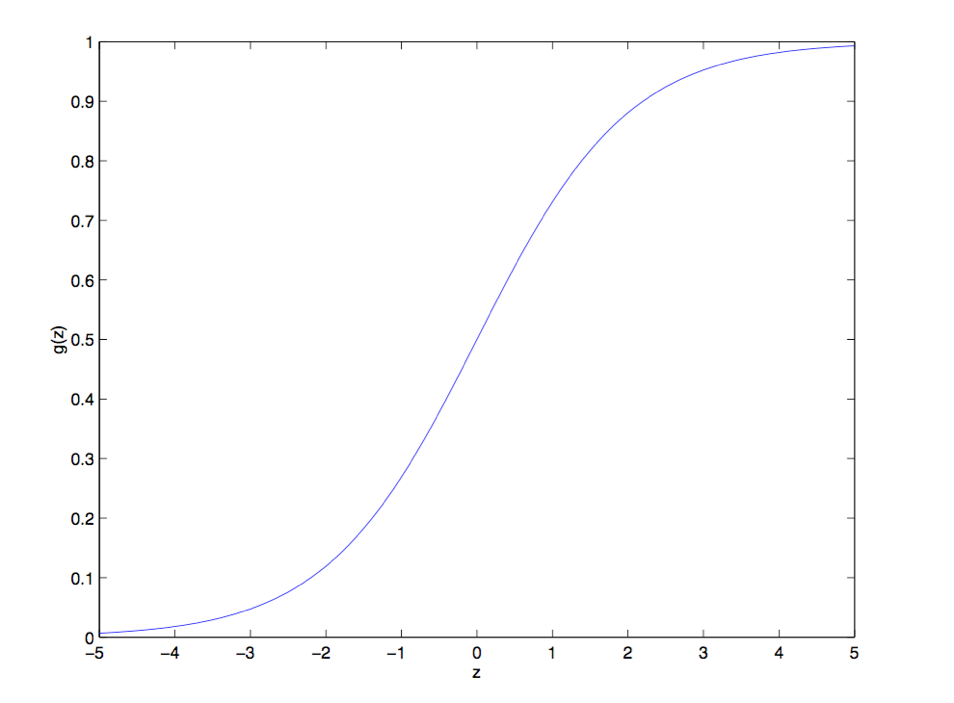
\includegraphics[height=7cm]{\pathroot/theory/GLM/images/sigmoid.png}
    \caption{sigmoid函数}
    \label{fig:sigmoid}
\end{figure}

函数可导:
\[
g'(z)={\frac {d}{dz}}{\frac {1}{1+e^{-\theta^Tx}}}=\lim_{{\Delta x}\to 0}{\frac {f(x+{\Delta x})-f(x)}{\Delta x}}
\]

对于一个二分类问题,可假设$h_{\theta}(x)$为其中一类的概率,即:
\[
P(y=1|x;\theta)=h_{\theta}(x)
               =h_{\theta}(x)^{1}(1-h_{\theta}(x))^{1-1}
               =h_{\theta}(x)^{y}(1-h_{\theta}(x))^{1-y}
\]

\[
P(y=0|x;\theta)=1-h_{\theta}(x)
               =h_{\theta}(x)^{0}(1-h_{\theta}(x))^{1-0}
               =h_{\theta}(x)^{y}(1-h_{\theta}(x))^{1-y}
\]


\begin{minted}[mathescape,
               numbersep=5pt,
               frame=lines,
               framesep=2mm]{python}
class SimpleLogisticRegression(object):
    def __init__(self, alpha, feature_num):
        pass
    def fit(self, X, y, verbose=False):
        last_target = -sys.maxint
        last_step = 0
        step = 0
        while True:
            step += 1
            # 计算梯度并更新参数
            target = sum(map(lambda py, ty: ty * math.log(py) + (1 - ty) * math.log(1 - py),
                             map(self.__sigmoid, X), y)) / len(X)
            if target - last_target > 1e-8:
                last_target = target
                last_step = step
            elif step - last_step >= 10:
                break
        target = sum(map(lambda py, ty: ty * math.log(py) + (1 - ty) * math.log(1 - py),
                         map(self.__sigmoid, X), y)) / len(X)
        return target


    def predict(self, X):
        pass
    def __sigmoid(self, x):
        pass
    def _check_columns(self, X):
        pass

if __name__ == "__main__":
    lr = SimpleLogisticRegression(0.1, 3)
    X = [[1, 3, 5], [2, 4, 6], [3, 5, 7], [4,  6, 8]]
    y = [0, 0, 1, 1]
    print lr.predict(X)
    lr.fit(X, y, verbose=True)
    print lr.predict(X)
\end{minted}

\begin{minted}[mathescape,
               numbersep=5pt,
               frame=lines,
               framesep=2mm]{python}
#coding: utf-8
#author: Ryan
"""
A simple Logistic Regression model.
"""
from __future__ import division
import sys
import os
import random
import math
import collections
import array
import operator

class SimpleLogisticRegression(object):
    def __init__(self, alpha, feature_num):
        """构造函数
        参数
        ---
        alpha: double
            学习率
        feature_num: int
            特征数量
        """
        self.__alpha = alpha
        self.__features_num = feature_num
        self.__coef = [0.] * self.__features_num
        self.__intercept = 0.

    def fit(self, X, y, verbose=False):
        """训练模型。
        返回值
        ------
            模型训练的最终log似然值。
        """
        last_target = -sys.maxint
        last_step = 0
        step = 0
        while True:
            step += 1
            gradient = [0.] * (self.__features_num + 1)
            for tx, ty in zip(X, y):
                delta = ty - self.__sigmoid(tx)
                for i, xi in enumerate(tx):
                    gradient[i] += delta * xi
                gradient[-1] += delta
            gradient = map(lambda g: g / len(X), gradient)

            self.__coef = map(lambda c, g: c + self.__alpha * g, self.__coef, gradient[:-1])
            self.__intercept += self.__alpha * gradient[-1]

            target = sum(map(lambda py, ty: ty * math.log(py) + (1 - ty) * math.log(1 - py),
                             map(self.__sigmoid, X), y)) / len(X)
            if target - last_target > 1e-8:
                last_target = target
                last_step = step
            elif step - last_step >= 10:
                break
            if verbose is True and step % 1000 == 0:
                sys.stderr.write("step %s: %.6f\n" % (step, target))
        target = sum(map(lambda py, ty: ty * math.log(py) + (1 - ty) * math.log(1 - py),
                         map(self.__sigmoid, X), y)) / len(X)
        if verbose is True:
            sys.stderr.write("Final training error: %.6f\n" % (target))
        return target

    def predict(self, X):
        """输出每个样本的预测值。
        返回值
        -----
            列表类型,长度与X的样本量相同。
        """
        if not self._check_columns(X):
            sys.stderr.write("The data to be evaluated can't match training data's features\n")
            return None
        return map(self.__sigmoid, X)

    def __sigmoid(self, x):
        """sigmoid函数,返回sigmoid函数值"""
        return 1. / (1 + math.exp(-sum(map(operator.mul, self.__coef, x)) - self.__intercept))

    def _check_columns(self, X):
        """检查每个样本的类型是否是数组或者列表类型,并且长度与特征数相等。
        返回值
        -----
            数据合法时,返回True,否则返回False。
        """
        for x in X:
            if not isinstance(x, (list, tuple, array.array)):
                return False
            if len(x) != self.__features_num:
                return False
        return True

if __name__ == "__main__":
    lr = SimpleLogisticRegression(0.1, 3)
    X = [[1, 3, 5], [2, 4, 6], [3, 5, 7], [4,  6, 8]]
    y = [0, 0, 1, 1]
    print lr.predict(X)
    lr.fit(X, y, verbose=True)
    print lr.predict(X)
\end{minted}



\begin{itemize}
\item 更简洁的形式: $P(y|x;\theta)={h_{\theta}(x)}^y(1-h_{\theta}(x))^{1-y}$
\item 假设$m$个训练样本独立,则样本集在参数${\theta}$给定下,出现的概率为
\begin{align*}
L(\theta)&=p(\vec y|X;\theta)\\
         &=\prod_{i=1}^{m}{p(y^{(i)} | x^{(i)};\theta)}\\
         &=\prod_{i=1}^{m}{(h_{\theta}(x^{(i)}))^{y^{(i)}}(1-h_{\theta}(x^{(i)}))^{(1-y^{(i)})}}
\end{align*}

\item 我们希望最大化概率$L({\theta})$,也即最大化log似然值:

\item 最大化一个目标值,可采用梯度上升法,沿着梯度方向不断迭代。梯度求解如下:

\item 随机梯度下降法求解:
\subitem ${\theta}_{j}:={\theta}_{j}+{\alpha}(y^{(i)}-h_{\theta}(x^{(i)}))x_{j}^{(i)}$

\item 思考:
\subitem 如果引入$L1$正则、$L2$正则,那么梯度又该怎么求解呢?
\subitem LR的梯度求解公式与线性回归的梯度求解公式看起来一样,有区别么?

\item L1:$cost(w)={\frac {1}{2m}}\left\|{Xw-y}\right\|^{2}+\lambda\|w\|_{1}$
,等价于
    $\min\limits_{w}{\frac {1}{2m}}\left\|{Xw-y}\right\|^{2}, s.t. \left\|w\right\|_{1}\le{C}$

\item L2:$cost(w)={\frac {1}{2m}}\left\|{Xw-y}\right\|^{2}+{\frac {\lambda}{2}}\|w\|_{2}^{2}$
,等价于
    $\min\limits_{w}{\frac {1}{2m}}\left\|{Xw-y}\right\|^{2}, s.t. \left\|w\right\|_{2}^{2}\le{C}$

\item 常用分类器的评价指标有:准确率(precision)、召回率(recall)、F值、正确率(accuracy)等
\end{itemize}

\begin{itemize}

\item 考虑ROC曲线图中的四个点。
    \subitem(1)第一个点(0,1),FPR=0, TPR=1,即FN=0,并且FP=0。
        \subsubitem 特点:正确分类所有的样本。
    \subitem(2)第二个点(1,0),FPR=1,TPR=0。
        \subsubitem 特点:成功错分了所有的样例。
    \subitem(3)第三个点(0,0),FPR=TPR=0,即FP=TP=0,
        \subsubitem 特点:分类器预测所有的样本都为负样本。
    \subitem(4)第四个点(1,1),分类器预测所有的样本都为正样本。
\item 结论:ROC曲线越接近左上角,该分类器的性能越好。
\item 考虑ROC曲线图中的虚线$y=x$上的点。这条对角线上的点表示的是一个采用随机猜测策略的分类器的结果。

\item ROC曲线的画法:对一个特定的测试数据集合,对分类模型输出的概率值设置不同的阈值,从而得到一组(FPR,TPR)点,以此连接这些点即可得到ROC曲线。
\item AUC(Area Under Curve):ROC曲线下的面积。
\item AUC值等于一个随机选择的正样本的预测值高于一个随机选择的负样本的概率。
\item ROC曲线的优点:当测试集中的正负样本的分布变化的时候,ROC曲线能够保持不变。

\item 在右图中,(a)和(c)为ROC曲线,(b)和(d)为\\
Precision-Recall曲线。(a)和(b)展示的是\\
分类其在原始测试集(正负样本分布平衡)\\
的结果,(c)和(d)是将测试集中负样本的数\\
量增加到原来的10倍后, 分类器的结果。可\\
以明显的看出,ROC曲线基本保持原貌,\\
而Precision-Recall曲线则变化较大。
\end{itemize}

\subsection{LR解决多分类问题}
基本思路:将多分类任务拆若干个二分类任务。学习时分别训练多个分类器,测试时对这多个分类器的预测结果进行集成以获得最终的多分类结果。

一般来说,有以下几种做法。

\subsubsection{一对一(OvO) }
以$C_{i}$与$C_{j}$的数据作为正反例训练一个分类器,共训练${\frac {N(N-1)}{2}}$个分类器
预测时将样本提交给所有分类器,获取${\frac {N(N-1)}{2}}$个结果,最终结果通过投票产生

\subsubsection{一对多(OvR)}
以$C_{i}$数据为正例,其余类别数据为负例,训练$N$个分类器

\subsubsection{其他}
如多对多(MvM)策略的ECOC编码


\section{Softmax Regression}
为LR在多分类上的推广。与LR一样,同属于广义线性模型(Generalized Linear Model)。

\[
P(y=i|x;{\theta})={\frac {e^{{\theta}_{i}^{T}x}}{\sum_{j=1}^{K}{e^{{\theta}_{j}^{T}x}}}}
\]

同样,考虑使得对数似然最大,则系统损失函数为:
\[
\ell(\theta)=-{\frac {1}{m}}\left[\sum\limits_{i=1}^{m}{\sum\limits_{j=1}^{K}{1\{y^{(i)}=j\}\log{\frac{e^{{\theta}_{j}^{T}{x^{(i)}}}}{\sum_{l=1}^{K}{e^{\theta_{l}^{T}x^{(i)}}}}}}}\right]
\]

加入正则项:
\[
\ell(\theta)=-{\frac {1}{m}}\left[\sum\limits_{i=1}^{m}{\sum\limits_{j=1}^{K}{1\{y^{(i)}=j\}\log{\frac{e^{{\theta}_{j}^{T}{x^{(i)}}}}{\sum_{l=1}^{K}{e^{\theta_{l}^{T}x^{(i)}}}}}}}\right]+
    {\frac {\lambda}{2}{\sum\limits_{i=1}^{K}{\sum\limits_{j=0}^{n}{\theta_{ij}^{2}}}}}
\]

考虑一个样本$(x,y)$,有$\ell(x,\hat{y})=-\sum\limits_{j=1}^{K}{1\{y=j\}\ln{\hat{y}_{j}}}$,令$a_{j}={\theta_{j}^{T}x}$,有
\begin{align*}
{\frac {\partial \ell(x,\hat{y})}{a_{j}}}&=\sum\limits_{i=1}^{K}{{\frac {\partial \ell(x,\hat{y})}{\partial \hat{y}_{i}}}{\frac {\partial \hat{y}_{i}}{\partial a_{j}}}}\\
                                         &=-\sum\limits_{i=1}^{K}{
                                                {\frac {1\{y=i\}}{\hat{y}_{i}}}
                                                {\frac {\partial \frac {e^{a_{i}}}{\sum_{l=1}^{K}{e^{a_{l}}}}}{\partial a_{j}}}}\\
                                         &=-\sum\limits_{i=1}^{K}{
                                                {\frac {1\{y=i\}}{\hat{y}_{i}}}
                                                {\frac {
                                                            e^{a_{i}} \cdot 1\{i=j\} \cdot {\left({\sum_{l=1}^{K}{e^{a_{l}}}}\right)}
                                                            -e^{a_{i}} \cdot e^{a_{j}}
                                                        }
                                                       {\left({\sum_{l=1}^{K}{e^{a_{l}}}}\right)^{2}}
                                                    }}\\
                                         &=\sum\limits_{i=1}^{K}{
                                                {\frac {1\{y=i\}}{\hat{y}_{i}}}
                                                {\frac {e^{a_{i}} \cdot e^{a_{j}}}
                                                       {\left({\sum_{l=1}^{K}{e^{a_{l}}}}\right)^{2}}
                                                    }}
                                            -\sum\limits_{i=1}^{K}{
                                                {\frac {1\{y=i\}}{\hat{y}_{i}}}
                                                {\frac {e^{a_{i}} \cdot 1\{i=j\} \cdot {\left({\sum_{l=1}^{K}{e^{a_{l}}}}\right)}}
                                                       {\left({\sum_{l=1}^{K}{e^{a_{l}}}}\right)^{2}}
                                                    }}\\
                                         &=\sum\limits_{i=1}^{K}{{\frac {1\{y=i\}}{\hat{y}_{i}}}{\hat{y}_{i}}{\hat{y}_{j}}}
                                            -\sum\limits_{i=1}^{K}{{\frac {1\{y=i\}}{\hat{y}_{i}}}{\hat{y}_{i}} \cdot 1\{i=j\}}\\
                                         &={\hat{y}_{j}}-\sum\limits_{i=1}^{K}{{1\{y=i\}}} \cdot 1\{i=j\}\\
                                         &={\hat{y}_{j}}-{1\{y=j\}} \\
\end{align*}

对于多分类问题,LR与softmax之间如何选择
\begin{itemize}
\item 如果待分的类别互斥,使用softmax
\item 如果类别有交叉,则使用LR进行投票分类
\item 例如
    \subitem 有四个类别的音乐,分别为:古典音乐、乡村音乐、摇滚乐和爵士乐
    \subitem 有四个类别如下:人声音乐、舞曲、影视原声、流行歌曲
\end{itemize}

\begin{itemize}
\item 实际工程中,LR很少使用连续特征。一般将连续特征离散化成多个取值为0/1的离散特征。
\subitem 0. 离散特征的增加和减少都很容易,易于模型的快速迭代;
\subitem 1. 稀疏向量内积乘法运算速度快,计算结果方便存储,容易扩展;
\subitem 2. 离散化后的特征对异常数据有很强的鲁棒性;
\subitem 3. 逻辑回归属于广义线性模型,表达能力受限;离散化相当于为模型引入了非线性,提升模型表达能力;
\subitem 4. 离散化后可以进行特征交叉,由$M+N$个变量变为$M*N$个变量,进一步引入非线性,提升表达能力;
\subitem 5. 特征离散化后,模型会更稳定;
\subitem 6. 特征离散化以后,起到了简化了逻辑回归模型的作用,降低了模型过拟合的风险。

\end{itemize}




\begin{itemize}
\item 监督学习:利用一组已知类别的样本调整分类器的参数,\\使其达到所要求性能的过程
\item 一些符号定义:

$x^{(i)}$:指数据集中的第$i$个样本的特征类数据。

$y^{(i)}$:指数据集中的第$i$个样本的目标值。

$\left(x^{(i)},y^{(i)}\right)$:表示一个样本实例。

$\left\{\left(x^{(i)},y^{(i)}\right), i=1,...,N\right\}$:表示一个数据集。
\\例如,对于手写体识别来说,图片的像素表示即为特征$x$,图片表示的数字即为目标值$y$。

\end{itemize}

对于红酒问题,
\begin{itemize}
\item 问题分析:
\\(1) 共有11个特征,可表示为11个变量:$x^{(i)}_1,x^{(i)}_2,...,x^{(i)}_{11}$。
\\(2) 目标只有一个评分,可表示为:$y^{(i)}$
\\(3) 问题可表示为优化问题:$argmin_{w}\sum_{i=1}^{N}(w_0 + w_1*x^{(i)}_1 + w_2*x^{(i)}_2 + w_{11}*x^{(i)}_{11} - y^{(i)})^2$

\item 用向量表示更加简洁:
\\(1) 特征表示为:$x^{(i)}=\left(\begin{array}{ccc}x^{(i)}_0,x^{(i)}_1,...,x^{(i)}_{11}\end{array}\right)^T$,其中$x^{(i)}_0=1$
\\(2) 权重系数表示为:$w=\left(\begin{array}{ccc}w_0,w_1,...,w_{11}\end{array}\right)^T$
\\(3) 问题表示为:$argmin_{w} \sum_{i=1}^{N}(w^Tx^{(i)}-y^{(i)})^2$

\end{itemize}

\begin{equation}
  s_{kk'}=
  \left(
  \begin{array}{ccc}
          h_{1k} &
          \cdots &
          h_{nk}
  \end{array}
  \right)
  \left(
  \begin{array}{ccc}
          \bar{q}_{11} & \cdots & \bar{q}_{12}\\
          \vdots & \ddots & \vdots\\
          \bar{q}_{n1} & \cdots & \bar{q}_{n2}
  \end{array}
  \right)
  \left(
  \begin{array}{c}
          h_{1k'} \\
          \vdots \\
          h_{nk'}
 \end{array}
 \right)
\end{equation}


%\\$x=\begin{matrix} 0 & 1 \end{matrix}$

\subsubsection{Linear Regression}
\begin{itemize}

\item 给定一份数据集$\left\{x_0^{(i)},x_1^{(i)},...,x_m^{(i)},y^{(i)}\right\}_{i=0}^{N-1}$,线性回归假设目标值$y^{(i)}$与特征$x^{(i)}$之间为线性关系,即:$$y^{(i)}=w_0x_0^{(i)}+w_1x_1^{(i)}+...+w_mx_m^{(i)}$$

\item 现实世界不存在完美线性相关的关系,总会有各\\
种各样的偏差存在。由大数定理,可假设真实值\\
总在理论值附近波动,误差符合高斯分布, 即:\\
$y^{(i)}=w_0x_0^{(i)}+w_1x_1^{(i)}+...+w_mx_m^{(i)}+\varepsilon^{(i)}$\\
其中,$\varepsilon^{(i)}\sim{\mathcal{N}}(0, \sigma^{2})$
%其中,$\varepsilon\sim{\mathcal{N}}(\mu, \sigma^{2})$

\item 假设训练集中一共有$N$个样本:

$X=\left(
\begin{array}{c}
        {(x^{(0)})}^T \\
        {(x^{(1)})}^T \\
        \vdots \\
        {(x^{(N-1)})}^T \\
\end{array}
\right)=\left(
\begin{array}{ccc}
        x_0^{(0)} & \cdots & x_m^{(0)} \\
        x_0^{(1)} & \cdots & x_m^{(1)} \\
        \vdots & \ddots & \vdots\\
        x_0^{(N-1)} & \cdots & x_m^{(N-1)}
\end{array}
\right)$
$w=\left(
\begin{array}{c}
        w^{(0)} \\
        w^{(1)} \\
        \vdots \\
        w^{(m)}
\end{array}
\right)$
$y=\left(
\begin{array}{c}
        y^{(0)} \\
        y^{(1)} \\
        \vdots \\
        y^{(N-1)}
\end{array}
\right)$

\item 线性回归的目标就是最小化预估值与真实值的差距,也即所求$w$满足:$$argmin \left\|{Xw-y}\right\|^{2}$$
\item 代数解:$w=(X^{T}X)^{-1}X^{T}y$
\end{itemize}


\begin{itemize}
\item 代数解非常优美:\\
(1) 当$X^{T}X$为满秩矩阵或正定矩阵时,上式有唯一解。\\
(2) 现实任务中往往不是满秩矩阵,即$X^{T}X$不可逆,原因有很多,例如:
    \begin{itemize}
    \item 存在冗余特征,例如特征之间相关
    \item 训练样本少,如特征数甚至超过样本数
    \end{itemize}
此时$w$有多个可行解,需要选择最佳$w$。 \\
(3) 此代数解运算复杂度高,当$n>10000$时开销过大。\\

\end{itemize}

\subparagraph{梯度下降}
介绍梯度下降的原理。
\subsection{理论}

\begin{itemize}
\item 想法:人类在学习的时候,都是渐进式学习,不断从错误中纠正自己的认知,从而越来越优秀。
\item 导数定义:$ {\frac {dy}{dx}}={\frac {df}{dx}}(x)={\frac {d}{dx}}f(x)=f'(x)=\lim_{{\Delta x}\to 0}{\frac {f(x+{\Delta x})-f(x)}{\Delta x}} $\\
有:$f(x+{\Delta x})-f(x)=f'(x){\Delta x}$
\\(1) 如果$f'(x)>0$:
\subitem 当${\Delta x}>0$时,$f(x+{\Delta x})-f(x)=f'(x){\Delta x}>0$;
\subitem 当${\Delta x}<0$时,$f(x+{\Delta x})-f(x)=f'(x){\Delta x}<0$
\\(2) 如果$f'(x)<0$:
\subitem 当${\Delta x}>0$时,$f(x+{\Delta x})-f(x)=f'(x){\Delta x}<0$;
\subitem 当${\Delta x}<0$时,$f(x+{\Delta x})-f(x)=f'(x){\Delta x}>0$
\item 结论:如果使$x$变化的方向与$f'(x)$一致,将会使得$f(x)$增加。
\end{itemize}

\begin{itemize}
\item 梯度:$\nabla f=\left({\frac {\partial f}{\partial x_{1}}},\dots ,{\frac {\partial f}{\partial x_{n}}}\right)$,其中$\left(\nabla f\right)_{i}={\frac {\partial f}{\partial x_{i}}}$
\item 梯度下降算法(Gradient Descent):沿梯度下降的方向求解极小值。
\item 算法过程:
\\(1) 初始化参数为任意值。例如线性回归中的$w$。
\\(2) 求解梯度。例如线性回归中,求解 $\nabla\left(\left\|{Xw-y}\right\|^{2}\right)$。
\\(3) 更新参数。例如线性回归中,更新参数$w$,\\使得$w=w-\alpha\nabla\left(\left\|{Xw-y}\right\|^{2}\right)$,$\alpha$称为学习率。
\\(4) 若达到指定迭代次数或者收敛条件,训练结束。\\否则,继续执行步骤(2)。
\end{itemize}

\begin{itemize}
\item 实际应用中,对梯度下降算法有很多变形或改进。
\item 随机梯度下降(stochastic gradient descent):每遇到
\\一个或者多个但不是整个样本集,就计算梯度,更新参数。
\item 算法过程:
\\(1) 初始化参数为任意值。例如线性回归中的$w$。
\\(2) 对样本集中的每个样本,做如下操作直接完成所有样本\\的遍历:
\subitem(2.1) 求解梯度。例如线性回归中,求解 $\nabla\left(\left\|{Xw-y}\right\|^{2}\right)$。
\subitem(2.2) 更新参数。例如线性回归中,更新参数$w$,使得$w=w-\alpha\nabla\left(\left\|{Xw-y}\right\|^{2}\right)$。
\\(3) 若达到指定迭代次数或者收敛条件,训练结束。否则,继续执行步骤(2)。
\end{itemize}

\begin{itemize}
\item 一个完整的有监督学习的开发流程:
\\(1) 获取数据,对数据做一些清洗、转换等操作。
\\(2) 将数据样本拆分成训练集、验证集和测试集。训练集用来训练模型,验证集用来评估模型效果和调参,测试集则用来评估最终的模型效果。
\\(3) 开发模型或直接使用开发好的模型工具,在训练集上进行训练。
\\(4) 获取训练好的模型,使用验证集评估其效果。如果没有达到预期,需要进一步对模型调参、获取新的特征等操作,直到满足训练效果为止。
\\(5) 使用训练好的模型,在测试集上评估其最终效果。

\item 对于葡萄酒质量预估任务来说,主要有以下过程(只使用白酒的数据):
\\(1) 获取数据集,对数据集做一些预处理操作。
\\(2) 将处理好的数据集分为训练集、验证集和测试集,比例为:0.7:0.2:0.1。
\\(3) 开发线性回归模型。
\\(4) 在训练集上训练线性模型,在验证集上验证模型效果。没有达到预期,需要调参,直到满足训练效果为止。
\\(5) 在测试集中获取最终效果。

\end{itemize}

$x'={\frac {x - x_{min}}{x_{max} - x_{min}}}$

\begin{itemize}
\item 正则项:为有效控制模型参数的复杂度,加入参数复杂度的惩罚项,以使得模型选择更加简单的参数。
\item L1正则:$cost(w)={\frac {1}{2N}}\left\|{Xw-y}\right\|^{2}+\lambda\|w\|_{1}$
\item L2正则:$cost(w)={\frac {1}{2N}}\left\|{Xw-y}\right\|^{2}+{\frac {\lambda}{2}}\|w\|_{2}^{2}$
\\

加入正则项后,梯度:
\item L1正则:$w=w-\alpha (w^{T}x^{(i)}-y^{(i)})x^{(i)} - \alpha\lambda w$
\item L2正则:$w=w-\alpha (w^{T}x^{(i)}-y^{(i)})x^{(i)} - \alpha\lambda sign(w)$
\end{itemize}

\begin{itemize}
\item 优化目标:$cost(w)={\frac {1}{2N}}\left\|{Xw-y}\right\|^{2}$
\item 对于单个样本来说:$cost(w)={\frac {1}{2}}\left({w^{T}x^{(i)}-y^{(i)}}\right)^{2}$
\item 单个样本的梯度为:$\nabla cost(w)=(w^{T}x^{(i)}-y^{(i)})x^{(i)}$
\item 梯度更新:$w=w-\alpha (w^{T}x^{(i)}-y^{(i)})x^{(i)}$
\item 样本特征的取值情况如右图所示
\item 特征归一化: $x'={\frac {x - x_{min}}{x_{max} - x_{min}}}$

\end{itemize}

\subsection{交叉验证{\color{red} TODO}}

交叉验证(Cross Validation),有的时候也称作循环估计(Rotation Estimation),是一种统计学上将数据样本切割成较小子集的实用方法,该理论是由Seymour Geisser提出的。

在模式识别(Pattern Recognition)和机器学习(Machine Learning)的相关研究中,经常会将整个数据集合分成两个部分,分别是训练集合和测试集合。假设X是集合全体,A是全集X的非空真子集,那么非空集合X\textbackslash{A}则是集合A在全集X中的补集。于是可以先在A上面做训练和分析,而集合X\textbackslash{A}则用来做测试和验证。一开始的集合A被称作训练集,而它的补集X\textbackslash{A}被称作验证集或者测试集。这里有一个重要的观点就是:只有训练集才可以使用在模型的训练之中,而测试集必须在模型训练完成之后才被用来评估模型的误差。

\subsubsection{HoldOut检验(Hold-Out Method)}
这个方法是将原始的数据集合X随机分成两个集合A和X\textbackslash{A},其中A作为训练集,X\textbackslash{A}作为测试集。先使用训练集训练模型,然后利用测试集验证模型的效果,记录最后的分类准确率作为Hold-Out下该模型的性能指标。比方说,处理时间序列模型是否准确的时候,把整个数据集合分成前后两部分,前部分占比70\%,后部分占比30\%。前部分来进行时间序列模型的训练,后部分用来测试改时间序列的准确性。其准确性可以用MAE,MAPE之类的统计指标来衡量。综上所述,该方法的好处就是处理起来简单,只需要把原始数据分成两个部分即可。但是从严格意义上来说,Hold-Out检验并不算是交叉检验(Cross Validation),因为该方法没有达到交叉检验的思想,而且最后验证准确性的高低和原始数组的分类有很大的关系,所以该方法得到的结果在某些场景中并不具备特别大的说服力。在Hold-Out检验不够有说服力的情形下,有人提出了交叉验证这一个重要思想。

\subsubsection{交叉检验的常见形式}
假设有一个未知模型有一个或者多个未知的参数,并且有一个训练集。操作的过程就是对该模型的参数进行调整,使得该模型能够最大的反映训练集的特征。如果模型因为训练集过小或者参数不合适而产生过度拟合的情况,测试集的测试效果就可以得到验证。交叉验证是一种能够预测模型拟合性能的有效方法。

\subsubsection{彻底的交叉验证(Exhaustive Cross Validation)}
彻底的交叉验证方法指的是遍历全集X的所有非空真子集A。换句话说也就是把A当作训练集,X\textbackslash{A}是测试集。如果X中有n个元素,那么非空真子集A的选择方法则是$2^{n}-2$,这个方法的时间复杂度是指数级别的。

\begin{itemize}
\item 留P验证(Leave-p-out Cross Validation)
留p验证(LpO CV)指的是使用全集X中的p个元素作为测试集,然后剩下的n-p个元素作为训练集。根据数学上的定理可以得到,p个元素的选择方法有n!/((n-p)!p!)个,其中n!表示n的阶乘。在这个意义下,留p验证的时间复杂度也是非常高的。当p=1的时候,留1验证(Leave-one-out Cross Validation)的复杂度恰好是n。

\item 不彻底的交叉验证(Non-exhaustive Cross Validation)
不彻底的交叉验证不需要考虑全集X的所有划分情况,这种方法是留p验证的一个近似验证算法。

\item k-fold交叉验证(K-fold Cross Validation)
在k-fold交叉验证中,全集X被随机的划分成k个同等大小的集合A1,...,Ak,并且|A1|=...=|Ak|。这里的|Ai|指的是集合Ai的元素个数,也就是集合的势。这个时候需要遍历i从1到k,把X\textbackslash{Ai}当作训练集合,Ai当作测试集合。根据模型的测试统计,可以得到Ai集合中测试错误的结果数量ni。如果全集X的势是n的话,可以得到该模型的错误率是E=(ni求和)/n.
为了提高模型的精确度,可以将k-fold交叉验证的上述步骤重复t次,每一次都是随机划分全集X。在t次测试中,会得到t个模型的错误率E1,...,Et。令e=(Ei求和)/t。这样该模型的错误率就是e。

注释:
一般来说,k=10的情况使用得最多。
当k=2的时候,也就是最简单的k-fold交叉验证,2-fold交叉验证。这个时候X是A1和A2的并集,首先A1当训练集并且A2当测试集,然后A2当训练集并且A1当测试集。2-fold交叉验证的好处就是训练集和测试集的势都非常大,每个数据要么在训练集中,要么在测试集中。
当k=n的时候,也就是n-fold交叉验证。这个时候就是上面所说的留一验证(Leave-one-out Cross Validation)。
\end{itemize}
综上所述,交叉验证(Cross Validation)的好处是可以从有限的数据中获得尽可能多的有效信息,从而可以从多个角度去学习样本,避免陷入局部的极值。在这个过程中,无论是训练样本还是测试样本都得到了尽可能多的学习。

一般模型的选择过程:
在了解了交叉验证的方法之后,可以来介绍一般模型的选择过程。通过采用不同的输入训练样本,来决定机器学习算法中包含的各个参数值,称作模型选择。下面伪代码表示了模型选择的一般流程。在这个算法中,最重要的就是第三个步骤中的误差评价。 
(1)准备候选的q个模型:M1,...,Mq。 
(2)对每个模型M1,...,Mq求解它的学习结果。 
(3)对每个学习结果的误差e1,...,eq进行计算。这里可以使用上面所说的k-fold交叉验证方法。 
(4)选择误差e1,...,eq最小的模型作为最终的模型。









交叉验证是一种用来评价一个统计分析的结果是否可以推广到一个独立的数据集上的技术。主要用于预测,即,想要估计一个预测模型的实际应用中的准确度。它是一种统计学上将数据样本切割成较小子集的实用方法。于是可以先在一个子集上做分析, 而其它子集则用来做后续对此分析的确认及验证。 

交叉验证的理论是由Seymour Geisser所开始的。 它对于防范testing hypotheses suggested by the data是非常重要的,特别是当后续的样本是危险、成本过高或不可能(uncomfortable science)去搜集。

一个交叉验证将样本数据集分成两个互补的子集,一个子集用于训练(分类器或模型)称为训练集(training set);另一个子集用于验证(分类器或模型的)分析的有效性称为测试集(testing set)。利用测试集来测试训练得到的分类器或模型,以此作为分类器或模型的性能指标。

得到高度预测精确度和低的预测误差,是研究的期望。为了减少交叉验证结果的可变性,对一个样本数据集进行多次不同的划分,得到不同的互补子集,进行多次交叉验证。取多次验证的平均值作为验证结果。

在给定的建模样本中,拿出大部分样本进行建模型,留小部分样本用刚建立的模型进行预报,并求这小部分样本的预报误差,记录它们的平方加和。这个过程一直进行,直到所有的样本都被预报了一次而且仅被预报一次。把每个样本的预报误差平方加和,称为PRESS(predicted Error Sum of Squares)。

\subsubsection{目的}
用交叉验证的目的是为了得到可靠稳定的模型。在建立PCR 或PLS 模型时,一个很重要的因素是取多少个主成分的问题?用cross validation 校验每个主成分下的PRESS值,选择PRESS值小的主成分数。或PRESS值不在变小时的主成分数

交叉验证的目的:假设分类器或模型有一个或多个未知的参数,并且设这个训练器(模型)与已有样本数据集(训练数据集)匹配。训练的过程是指优化模型的参数,以使得分类器或模型能够尽可能的与训练数据集匹配。我们在同一数据集总体中,取一个独立的测试数据集。
\subsubsection{常见类型的交叉验证}
\begin{itemize}
\item 重复随机子抽样验证。
    \subitem 做法:将数据集随机的划分为训练集和测试集。对每一个划分,用训练集训练分类器或模型,用测试集评估预测的精确度。进行多次划分,用均值来表示效能。
    \subitem 优点:与k倍交叉验证相比,这种方法的与k无关。
    \subitem 缺点:有些数据可能从未做过训练或测试数据;而有些数据不止一次选为训练或测试数据。
\item 2、K倍交叉验证(K>=2)。
    \subitem 做法:将样本数据集随机划分为K个子集(一般是均分),将一个子集数据作为测试集,其余的K-1组子集作为训练集;将K个子集轮流作为测试集,重复上述过程,这样得到了K个分类器或模型,并利用测试集得到了K个分类器或模型的分类准确率。用K个分类准确率的平均值作为分类器或模型的性能指标。10-倍交叉证实是比较常用的。
    \subitem 优点:每一个样本数据都即被用作训练数据,也被用作测试数据。避免的过度学习和欠学习状态的发生,得到的结果比较具有说服力。
\item 3、留一法交叉验证。
    \subitem 做法:假设样本数据集中有N个样本数据。将每个样本单独作为测试集,其余N-1个样本作为训练集,这样得到了N个分类器或模型,用这N个分类器或模型的分类准确率的平均数作为此分类器的性能指标。
    \subitem 优点:每一个分类器或模型都是用几乎所有的样本来训练模型,最接近样本,这样评估所得的结果比较可靠。实验没有随机因素,整个过程是可重复的。
    \subitem 缺点:计算成本高,当N非常大时,计算耗时。
\end{itemize}

\subsubsection{训练集和测试集的选取}
\begin{itemize}
\item 1、训练集中样本数量要足够多,一般至少大于总样本数的50%。
\item 2、训练集和测试集必须从完整的数据集中均匀取样。均匀取样的目的是希望减少训练集、测试集与原数据集之间的偏差。当样本数量足够多时,通过随机取样,便可以实现均匀取样的效果。(随机取样,可重复性差)
\end{itemize}

\ifx\mlbook\undefined
    \end{document}
\fi


\ifx\mlbook\undefined
    \documentclass[10pt,a4paper]{ctexbook}
    \providecommand{\pathroot}{../..}

    \usepackage[CJKbookmarks,colorlinks,linkcolor=red]{hyperref}
    \usepackage{geometry}
    \usepackage{amsmath}

    \geometry{left=3.0cm,right=3.0cm,top=2.5cm,bottom=2.5cm}
    \setmainfont{SimSun}
    \XeTeXlinebreaklocale "zh"
    \XeTeXlinebreakskip = 0pt plus 1pt minus 0.1pt

    \begin{document}
    \setlength{\baselineskip}{20pt}
    \title{Learning To Rank}
    \author{Donald Cheung\\jianzhang9102@gmail.com}
    \date{Sep 8, 2017}
    \maketitle
    \tableofcontents
\fi

\chapter{Learning To Rank}
\href{https://www.microsoft.com/en-us/research/wp-content/uploads/2016/02/MSR-TR-2010-82.pdf}{From RankNet to LambdaRank to LambdaMART: An Overview}


\ifx\mlbook\undefined
    \end{document}
\fi

\chapter{Tree Models}
\chapter{Boosting}
\chapter{矩阵分解}
\chapter{浅层语义分析}
    \section{LSA}
    \section{PLSA}
    \section{LDA}
\ifx\mlbook\undefined
    \documentclass[10pt,a4paper]{ctexbook}
    \providecommand{\pathroot}{../..}

    \usepackage[CJKbookmarks,colorlinks,linkcolor=red]{hyperref}
    \usepackage{geometry}
    \usepackage{amsmath}

    \geometry{left=3.0cm,right=3.0cm,top=2.5cm,bottom=2.5cm}
    \setmainfont{SimSun}
    \XeTeXlinebreaklocale "zh"
    \XeTeXlinebreakskip = 0pt plus 1pt minus 0.1pt

    \begin{document}
    \setlength{\baselineskip}{20pt}
    \title{评估指标}
    \author{Donald Cheung\\jianzhang9102@gmail.com}
    \date{Sep 13, 2017}
    \maketitle
    \tableofcontents
\fi

\chapter{评估指标}

\section{准确率}
\section{召回率}
\section{F值}
\section{AUC}
\section{BLEU}

\ifx\mlbook\undefined
    \end{document}
\fi



\part{机器学习的工具}
\ifx\mlbook\undefined
    \documentclass[10pt,a4paper]{ctexbook}
    \providecommand{\pathroot}{../..}

    \usepackage[CJKbookmarks,colorlinks,linkcolor=red]{hyperref}
    \usepackage{geometry}
    \usepackage{amsmath}
    \usepackage{minted}

    \geometry{left=3.0cm,right=3.0cm,top=2.5cm,bottom=2.5cm}
    \setmainfont{SimSun}
    \XeTeXlinebreaklocale "zh"
    \XeTeXlinebreakskip = 0pt plus 1pt minus 0.1pt

    \begin{document}
    \setlength{\baselineskip}{20pt}
    \title{Python}
    \author{Donald Cheung\\jianzhang9102@gmail.com}
    \date{Oct 12, 2017}
    %\maketitle
    \tableofcontents
\fi

\chapter{Python}
Python是一种计算机程序设计语言。你可能已经听说过很多种流行的编程语言,比如非常难学的C语言,非常流行的Java语言,适合初学者的Basic语言,适合网页编程的JavaScript语言等等。

那Python是一种什么语言?

首先,我们普及一下编程语言的基础知识。用任何编程语言来开发程序,都是为了让计算机干活,比如下载一个MP3,编写一个文档等等,而计算机干活的CPU只认识机器指令,所以,尽管不同的编程语言差异极大,最后都得``翻译"成CPU可以执行的机器指令。而不同的编程语言,干同一个活,编写的代码量,差距也很大。

比如,完成同一个任务,C语言要写1000行代码,Java只需要写100行,而Python可能只要20行。

所以Python是一种相当高级的语言。

你也许会问,代码少还不好?代码少的代价是运行速度慢,C程序运行1秒钟,Java程序可能需要2秒,而Python程序可能就需要10秒。

那是不是越低级的程序越难学,越高级的程序越简单?表面上来说,是的,但是,在非常高的抽象计算中,高级的Python程序设计也是非常难学的,所以,高级程序语言不等于简单。

但是,对于初学者和完成普通任务,Python语言是非常简单易用的。连Google都在大规模使用Python,你就不用担心学了会没用。

用Python可以做什么?可以做日常任务,比如自动备份你的MP3;可以做网站,很多著名的网站包括YouTube就是Python写的;可以做网络游戏的后台,很多在线游戏的后台都是Python开发的。总之就是能干很多很多事啦。

Python当然也有不能干的事情,比如写操作系统,这个只能用C语言写;写手机应用,只能用Objective-C(针对iPhone)和Java(针对Android);写3D游戏,最好用C或C++。

\section{Python简介}
\subsection{Python是什么}
Python是著名的``龟叔" Guido van Rossum在1989年圣诞节期间,为了打发无聊的圣诞节而编写的一个编程语言。

现在,全世界差不多有600多种编程语言,但流行的编程语言也就那么20来种。有很多衡量编程语言流行度的方法,比较出名的有TIOBE编程语言排行榜(\ref{fig:TIOBE_INDEX_2017}、\ref{fig:TIOBE_Index_for_January_2017}、\ref{fig:TIOBE_Top10_LANGUAGE_EVOLUTION})、PYPL编程语言人气指数(\ref{fig:PYPL_INDEX_2017}、\ref{fig:PYPL_PopularitY_of_Programming_Language})、RedMonk编程语言排行榜(\ref{fig:REDMONK_RANKING_2017})\footnote{参考链接:\href{https://www.codingame.com/blog/top-programming-languages-to-learn-in-2017/}{TOP PROGRAMMING LANGUAGES TO LEARN IN 2017}}。

\begin{figure}[ht]
  \centering
  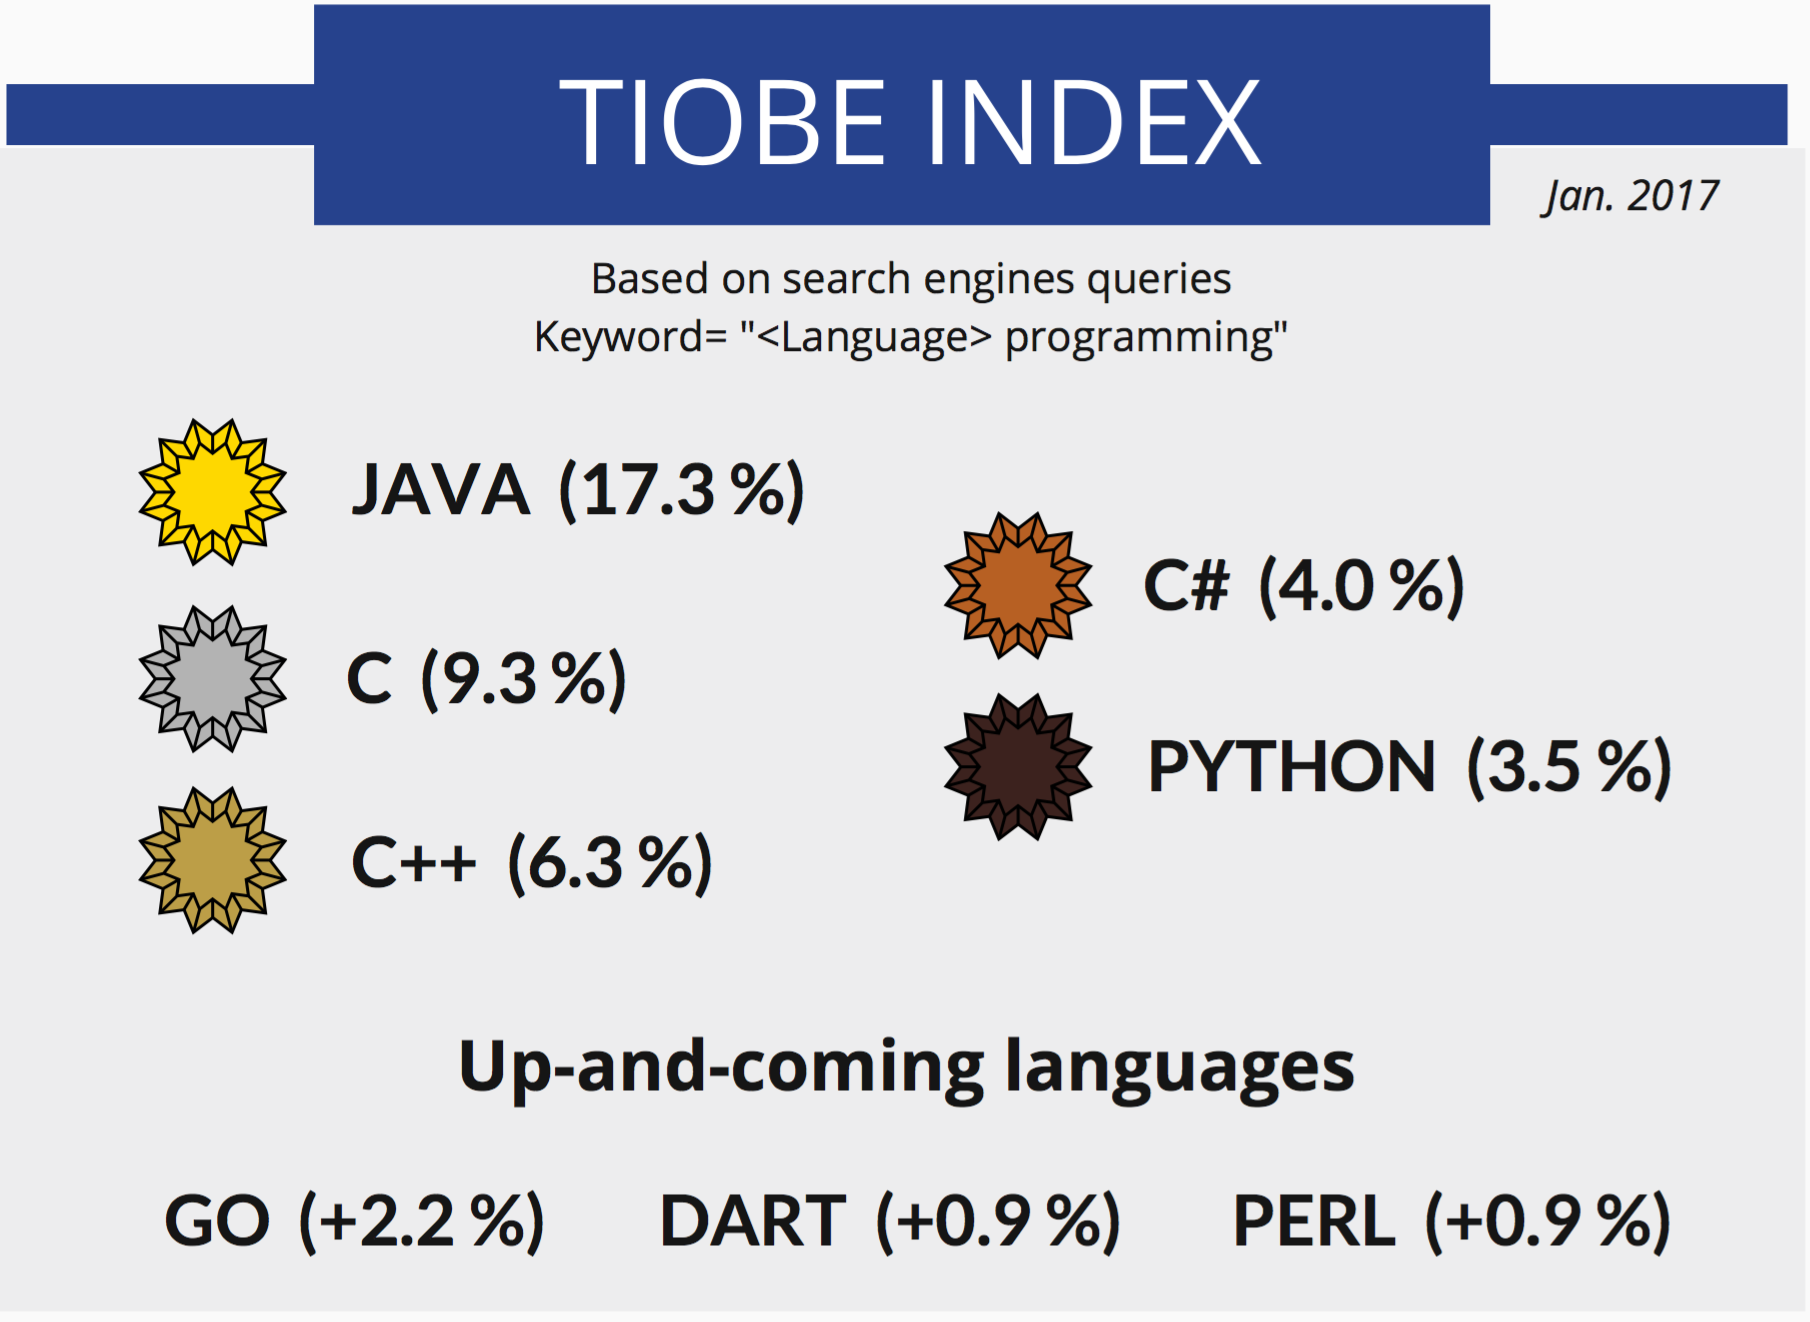
\includegraphics[scale=0.3]{\pathroot/tools/python/images/TIOBE_INDEX_2017.png}
  \caption{2017年TIOBE编程语言排行榜}
  \label{fig:TIOBE_INDEX_2017}
\end{figure}

\begin{figure}[ht]
  \centering
  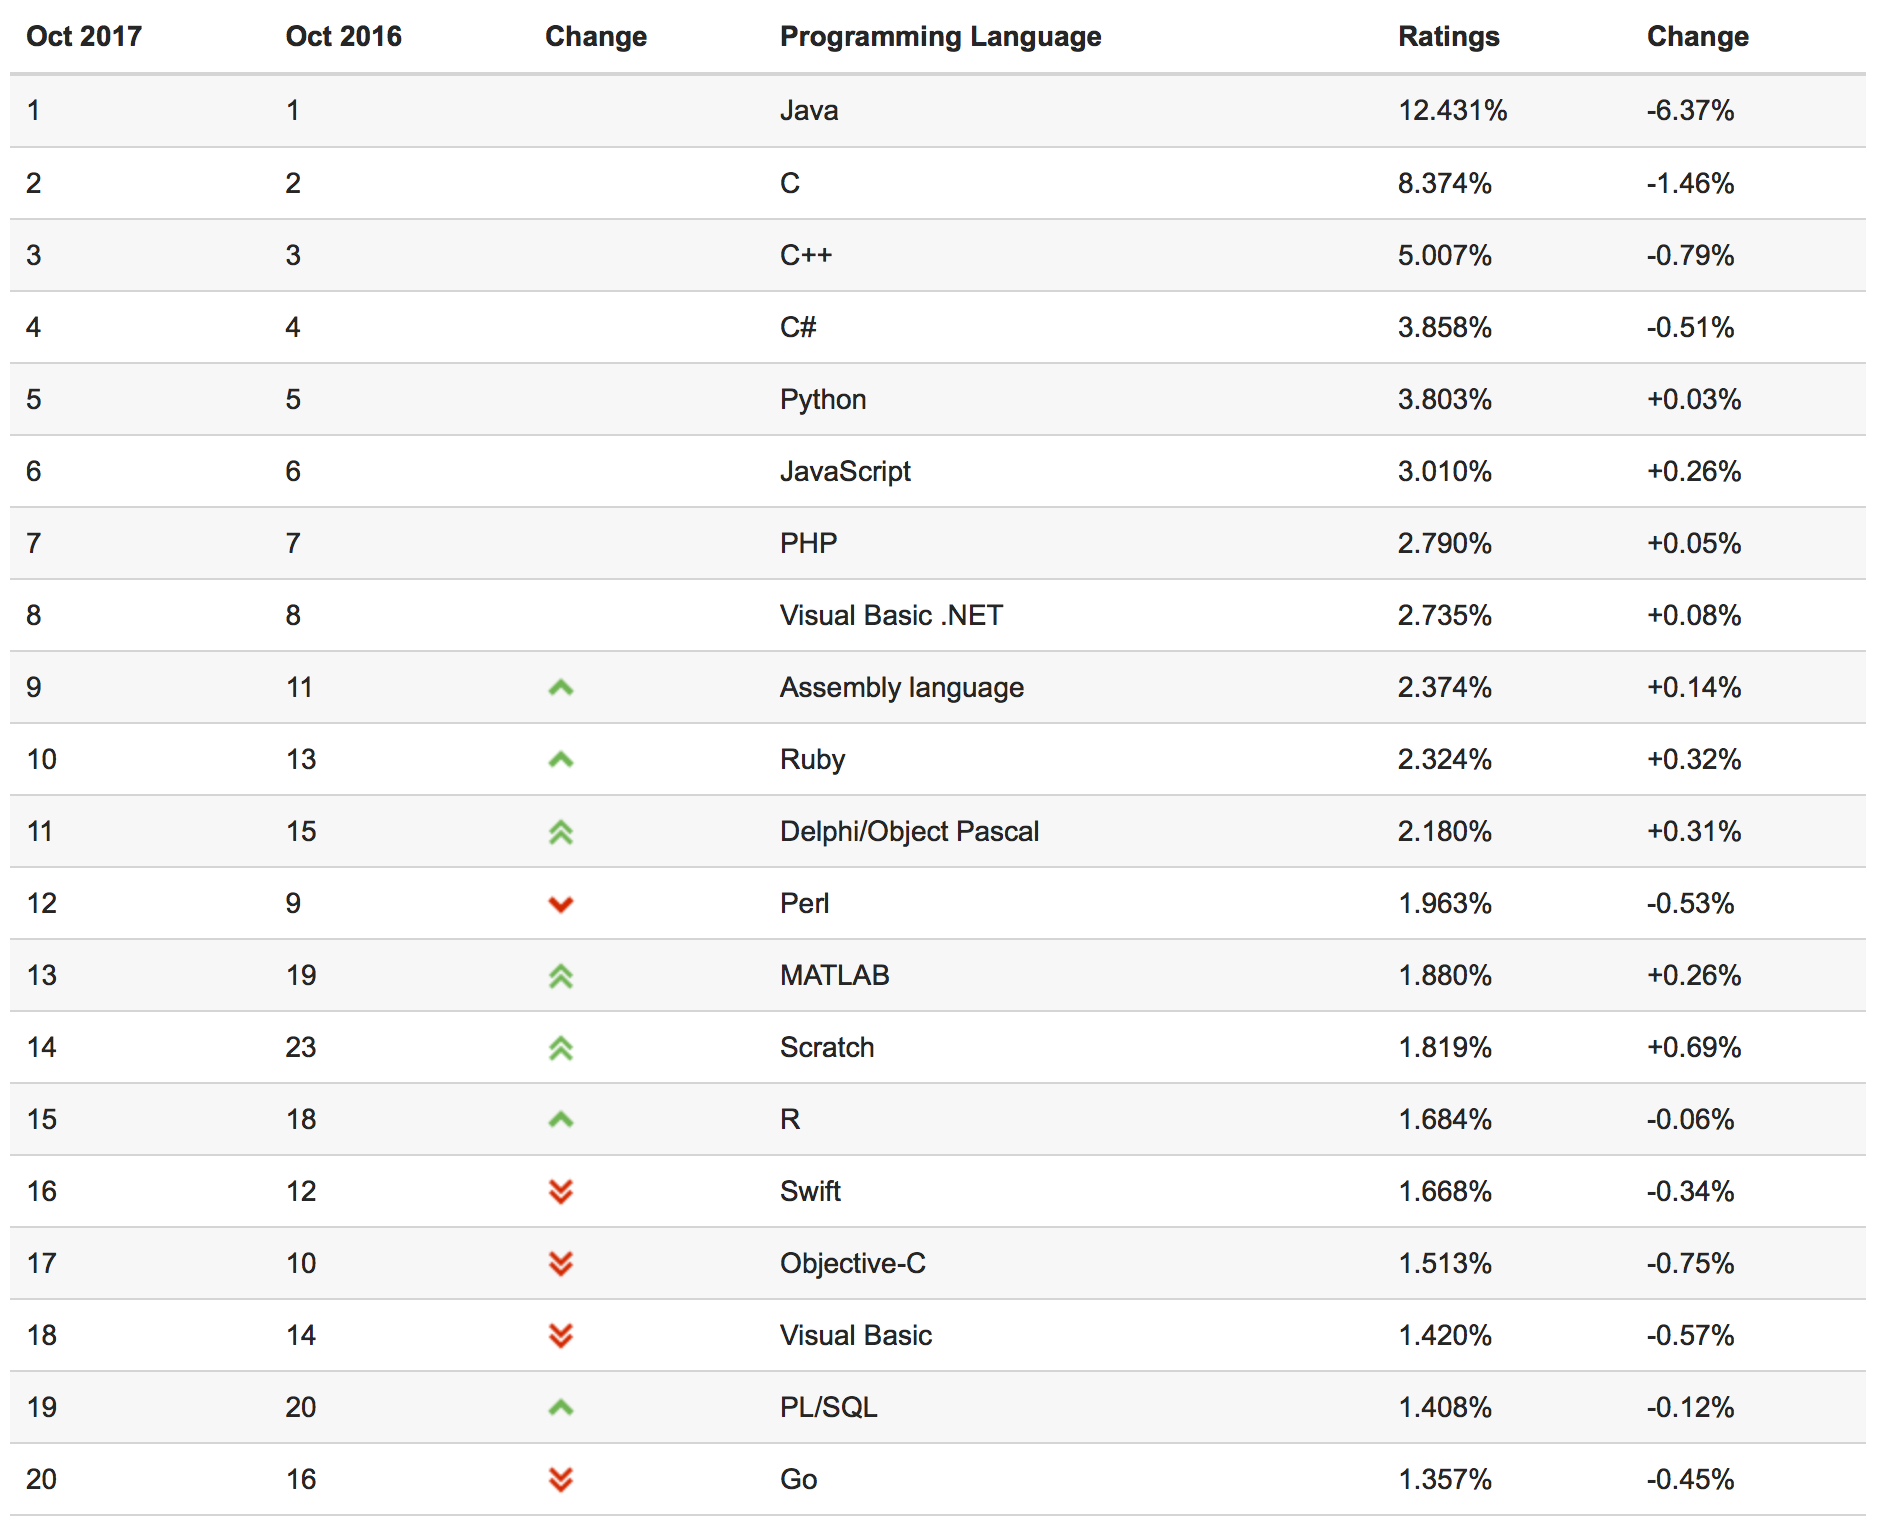
\includegraphics[scale=0.4]{\pathroot/tools/python/images/TIOBE_Index_for_January_2017.png}
  \caption{2017年1月TIOBE编程语言排行榜,来源:\href{http://www.tiobe.com/tiobe-index//}{TIOBE Index for January 2017}}
  \label{fig:TIOBE_Index_for_January_2017}
\end{figure}

\begin{figure}[ht]
  \centering
  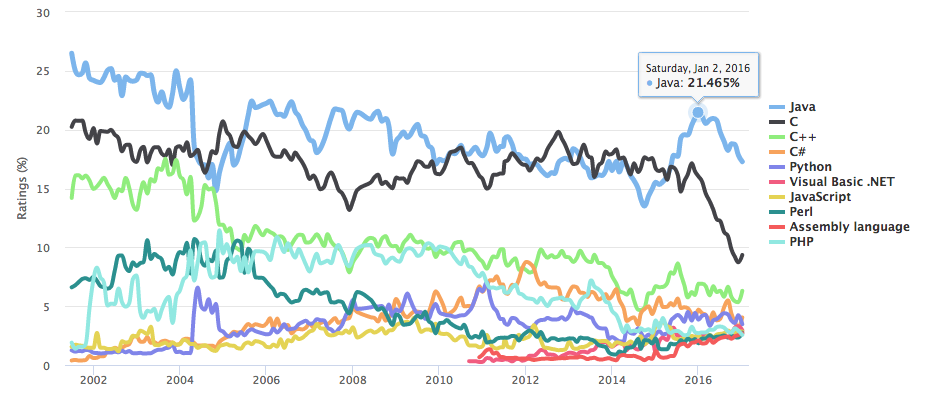
\includegraphics[scale=0.5]{\pathroot/tools/python/images/Evolution_of_the_top_10_languages_according_to_Tiobe.png}
  \caption{2017年TIOBE十大编程语言的演变,来源:\href{http://www.tiobe.com/tiobe-index//}{TIOBE Index for January 2017}}
  \label{fig:TIOBE_Top10_LANGUAGE_EVOLUTION}
\end{figure}

\begin{figure}[ht]
  \centering
  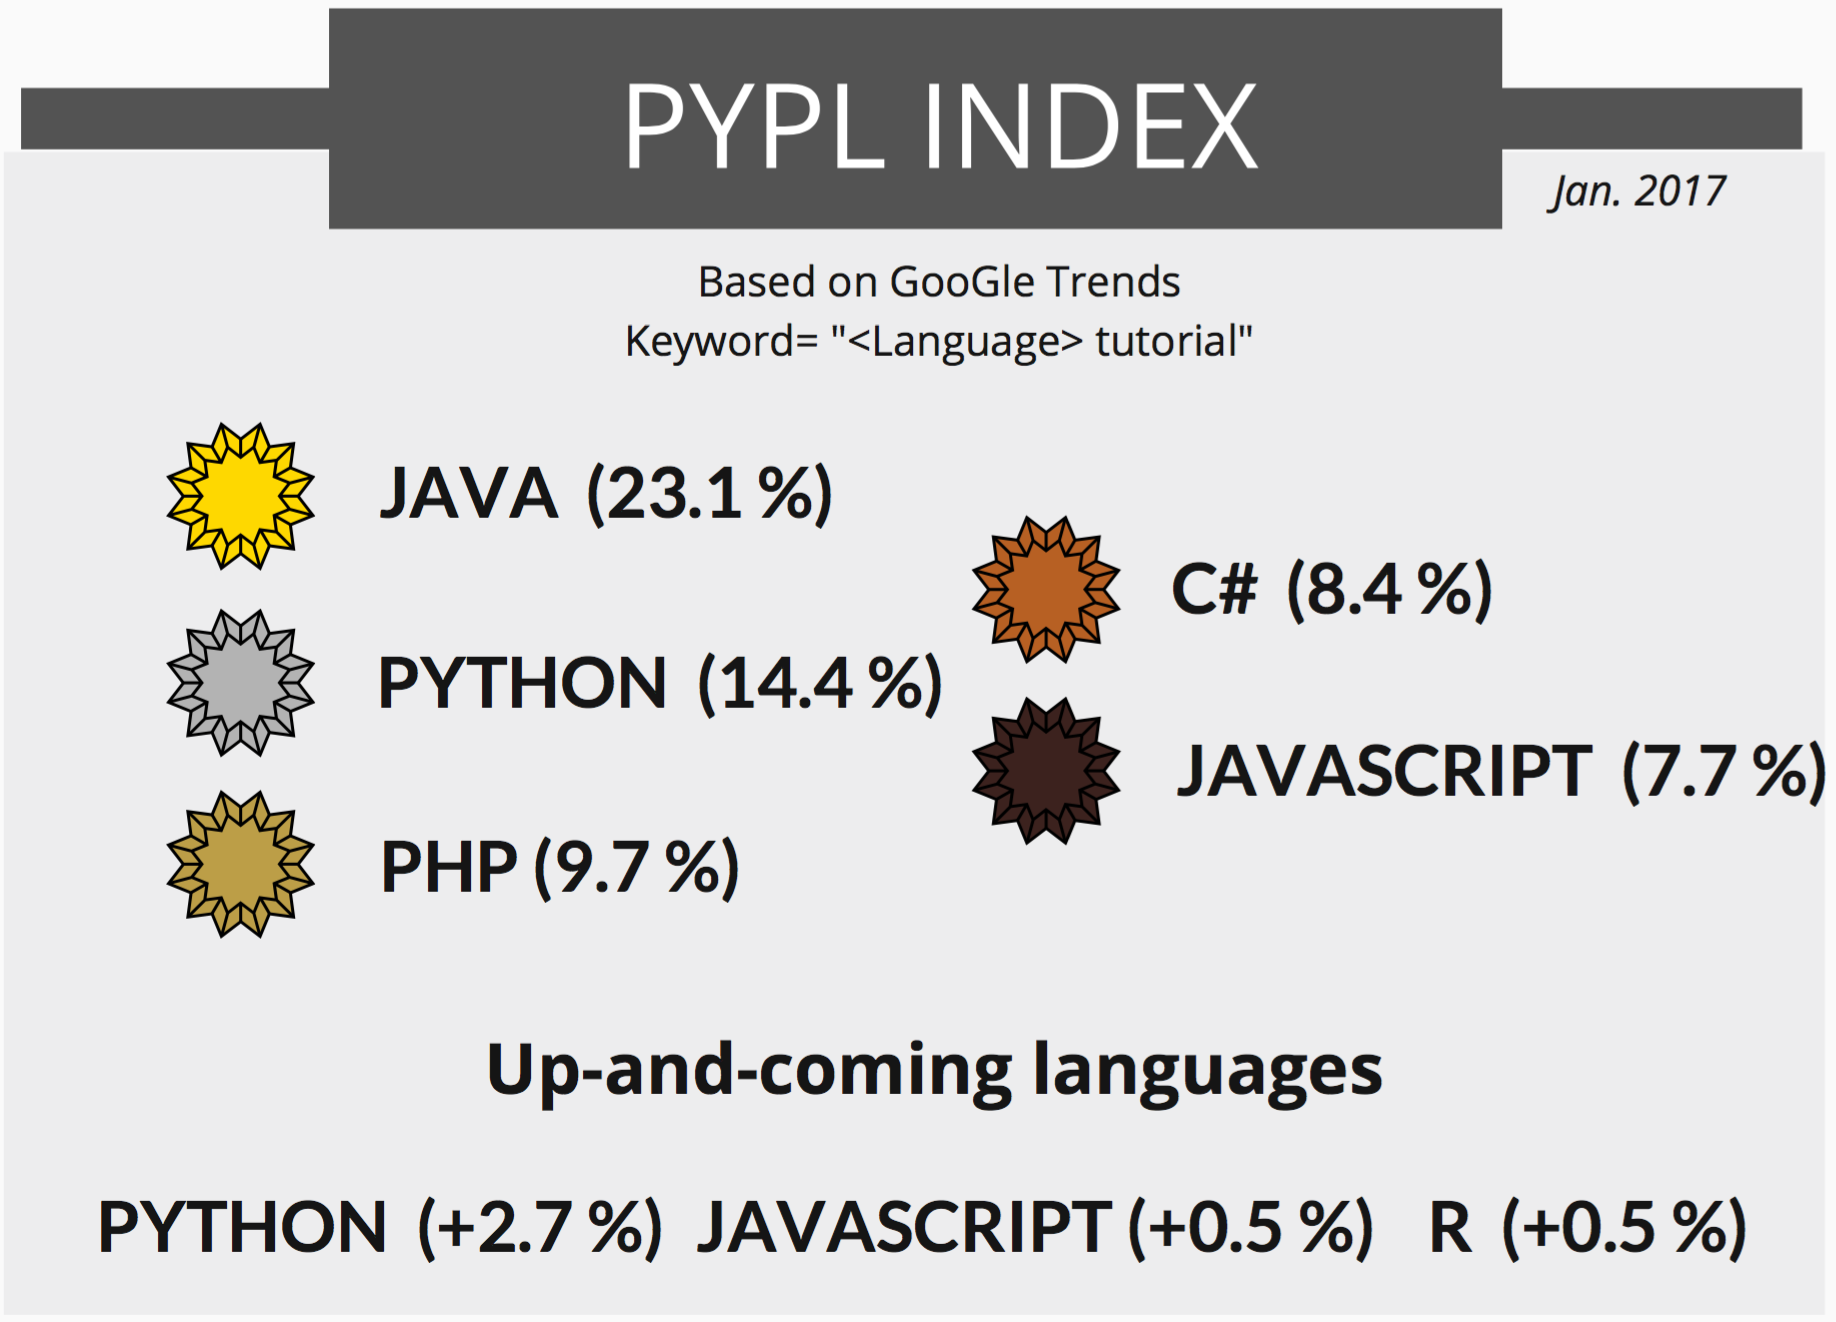
\includegraphics[scale=0.3]{\pathroot/tools/python/images/PYPL_INDEX_2017.png}
  \caption{2017年PYPL编程语言人气指数}
  \label{fig:PYPL_INDEX_2017}
\end{figure}

\begin{figure}[ht]
  \centering
  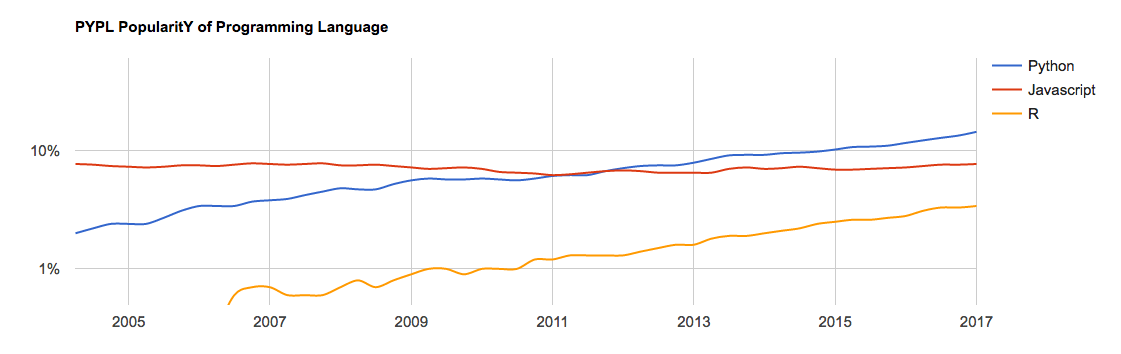
\includegraphics[scale=0.4]{\pathroot/tools/python/images/PYPL_PopularitY_of_Programming_Language.png}
  \caption{2017年PYPL编程语言人气指数,来源:\href{http://pypl.github.io/PYPL.html}{PYPL PopularitY of Programming Language Index, January 2017}}
  \label{fig:PYPL_PopularitY_of_Programming_Language}
\end{figure}


\begin{figure}[ht]
  \centering
  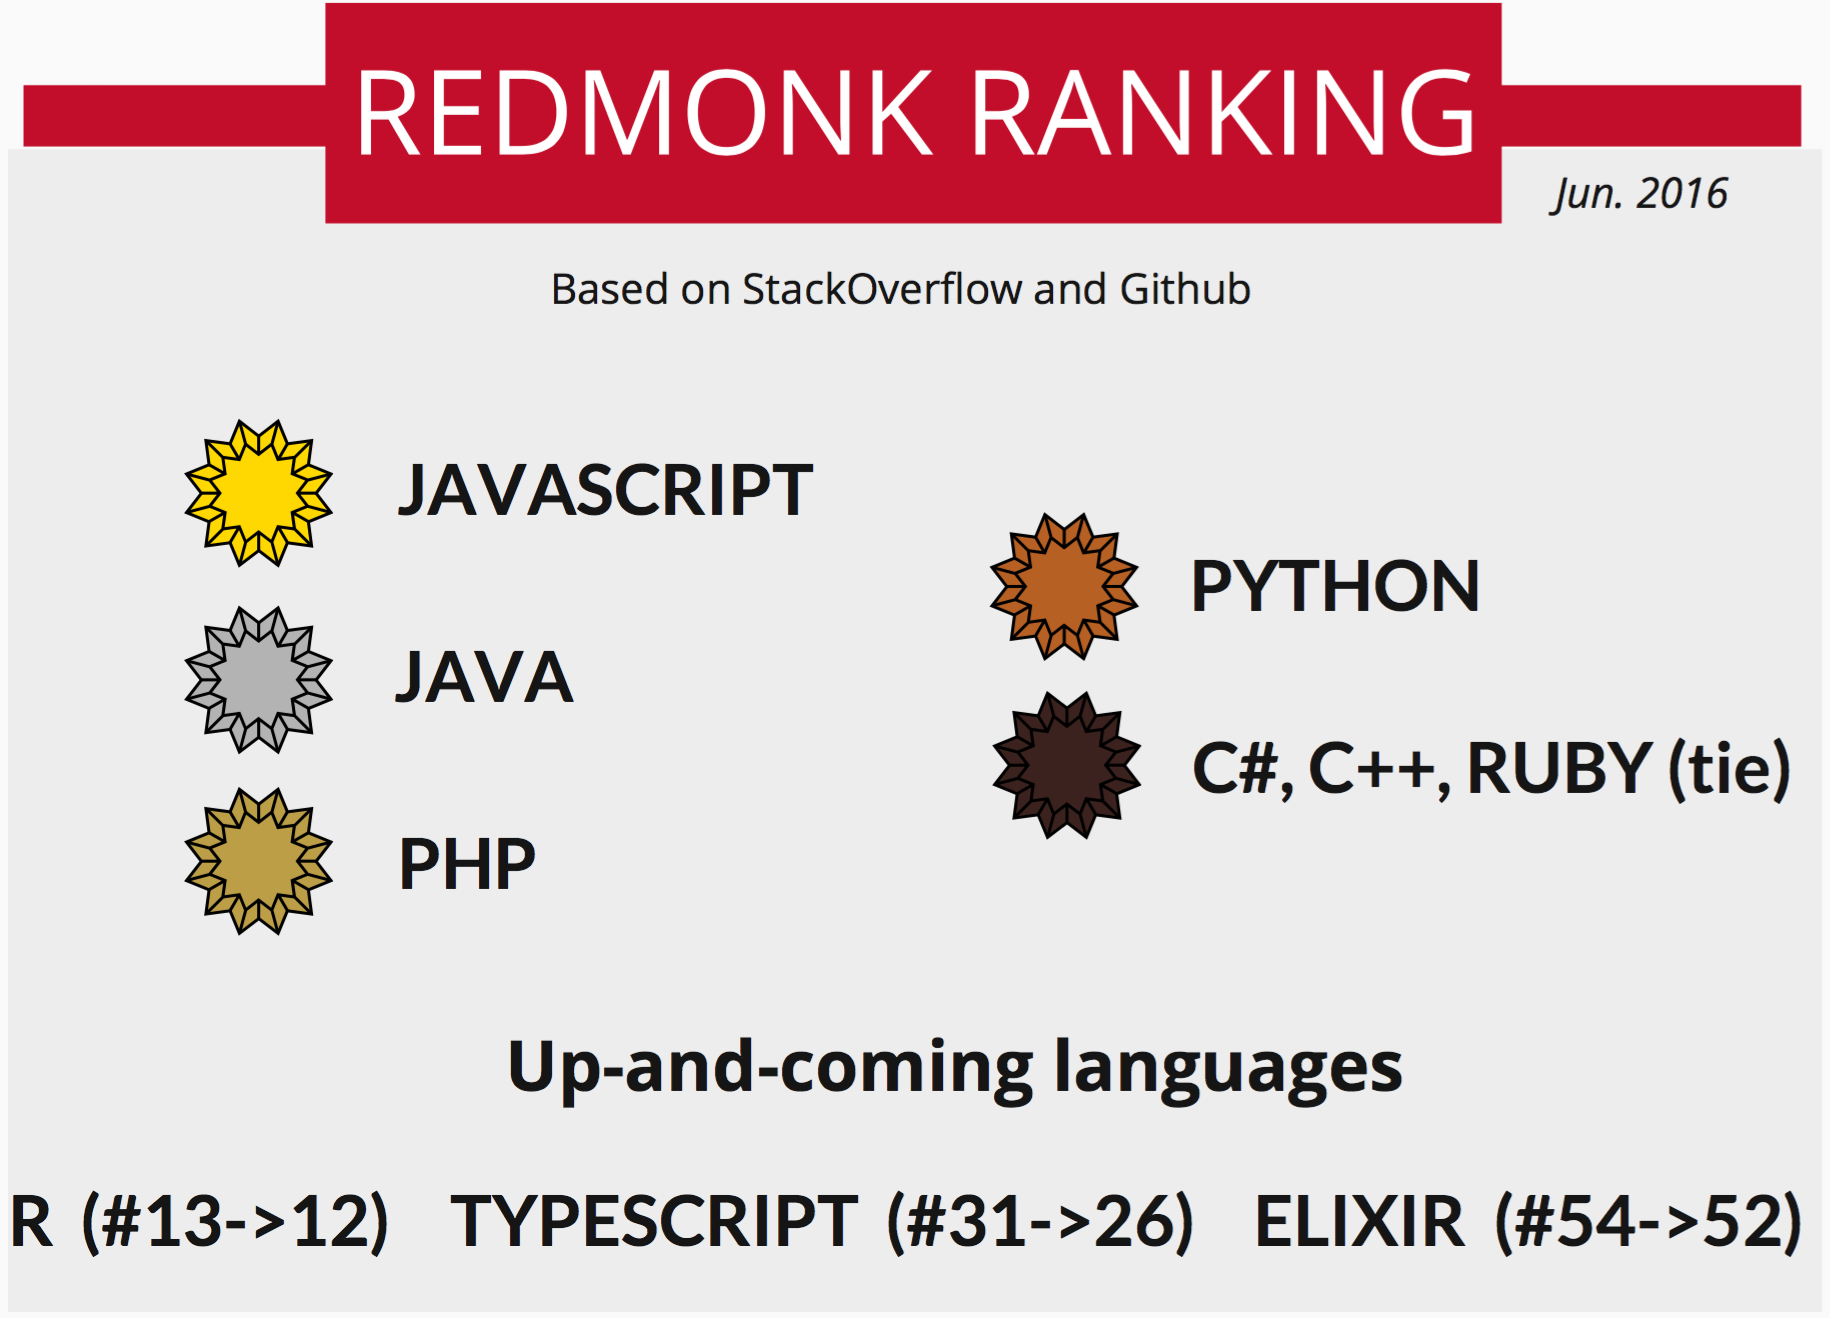
\includegraphics[scale=0.3]{\pathroot/tools/python/images/REDMONK_RANKING_2017.png}
  \caption{RedMonk编程语言排行榜}
  \label{fig:REDMONK_RANKING_2017}
\end{figure}

总的来说,这几种编程语言各有千秋。C语言是可以用来编写操作系统的贴近硬件的语言,所以,C语言适合开发那些追求运行速度、充分发挥硬件性能的程序。而Python是用来编写应用程序的高级编程语言。

当你用一种语言开始作真正的软件开发时,你除了编写代码外,还需要很多基本的已经写好的现成的东西,来帮助你加快开发进度。比如说,要编写一个电子邮件客户端,如果先从最底层开始编写网络协议相关的代码,那估计一年半载也开发不出来。高级编程语言通常都会提供一个比较完善的基础代码库,让你能直接调用,比如,针对电子邮件协议的SMTP库,针对桌面环境的GUI库,在这些已有的代码库的基础上开发,一个电子邮件客户端几天就能开发出来。

Python就为我们提供了非常完善的基础代码库,覆盖了网络、文件、GUI、数据库、文本等大量内容,被形象地称作``内置电池(batteries included)"。用Python开发,许多功能不必从零编写,直接使用现成的即可。

除了内置的库外,Python还有大量的第三方库,也就是别人开发的,供你直接使用的东西。当然,如果你开发的代码通过很好的封装,也可以作为第三方库给别人使用。

许多大型网站就是用Python开发的,例如YouTube、Instagram,还有国内的豆瓣。很多大公司,包括Google、Yahoo等,甚至NASA(美国航空航天局)都大量地使用Python。

龟叔给Python的定位是``优雅"、``明确"、``简单",所以Python程序看上去总是简单易懂,初学者学Python,不但入门容易,而且将来深入下去,可以编写那些非常非常复杂的程序。

总的来说,Python的哲学就是简单优雅,尽量写容易看明白的代码,尽量写少的代码。如果一个资深程序员向你炫耀他写的晦涩难懂、动不动就几万行的代码,你可以尽情地嘲笑他。

那Python适合开发哪些类型的应用呢?

首选是网络应用,包括网站、后台服务等等;

其次是许多日常需要的小工具,包括系统管理员需要的脚本任务等等;

另外就是把其他语言开发的程序再包装起来,方便使用。

最后说说Python的缺点。

任何编程语言都有缺点,Python也不例外。优点说过了,那Python有哪些缺点呢?

第一个缺点就是运行速度慢,和C程序相比非常慢,因为Python是解释型语言,你的代码在执行时会一行一行地翻译成CPU能理解的机器码,这个翻译过程非常耗时,所以很慢。而C程序是运行前直接编译成CPU能执行的机器码,所以非常快。

但是大量的应用程序不需要这么快的运行速度,因为用户根本感觉不出来。例如开发一个下载MP3的网络应用程序,C程序的运行时间需要0.001秒,而Python程序的运行时间需要0.1秒,慢了100倍,但由于网络更慢,需要等待1秒,你想,用户能感觉到1.001秒和1.1秒的区别吗?这就好比F1赛车和普通的出租车在北京三环路上行驶的道理一样,虽然F1赛车理论时速高达400公里,但由于三环路堵车的时速只有20公里,因此,作为乘客,你感觉的时速永远是20公里。

不要在意程序运行速度

第二个缺点就是代码不能加密。如果要发布你的Python程序,实际上就是发布源代码,这一点跟C语言不同,C语言不用发布源代码,只需要把编译后的机器码(也就是你在Windows上常见的xxx.exe文件)发布出去。要从机器码反推出C代码是不可能的,所以,凡是编译型的语言,都没有这个问题,而解释型的语言,则必须把源码发布出去。

这个缺点仅限于你要编写的软件需要卖给别人挣钱的时候。好消息是目前的互联网时代,靠卖软件授权的商业模式越来越少了,靠网站和移动应用卖服务的模式越来越多了,后一种模式不需要把源码给别人。

再说了,现在如火如荼的开源运动和互联网自由开放的精神是一致的,互联网上有无数非常优秀的像Linux一样的开源代码,我们千万不要高估自己写的代码真的有非常大的``商业价值"。那些大公司的代码不愿意开放的更重要的原因是代码写得太烂了,一旦开源,就没人敢用他们的产品了。

当然,Python还有其他若干小缺点,请自行忽略,就不一一列举了。

\subsection{安装Python}
因为Python是跨平台的,它可以运行在Windows、Mac和各种Linux/Unix系统上。在Windows上写Python程序,放到Linux上也是能够运行的。

要开始学习Python编程,首先就得把Python安装到你的电脑里。安装后,你会得到Python解释器(就是负责运行Python程序的),一个命令行交互环境,还有一个简单的集成开发环境。

目前,Python有两个版本,一个是2.x版,一个是3.x版,这两个版本是不兼容的,因为现在Python正在朝着3.x版本进化,在进化过程中,大量的针对2.x版本的代码要修改后才能运行,所以,目前有许多第三方库还暂时无法在3.x上使用。

\section{Python基础}
\subsection{第一个Python程序}
在交互式环境的提示符>>>下,直接输入代码,按回车,就可以立刻得到代码执行结果。
\begin{minted}[mathescape,
               numbersep=5pt,
               frame=lines,
               framesep=2mm]{python}
Python 2.7.12 (default, Dec  1 2016, 20:44:50) 
[GCC 4.2.1 Compatible Apple LLVM 8.0.0 (clang-800.0.42.1)] on darwin
Type "help", "copyright", "credits" or "license" for more information.
>>> print 'Hello World'
Hello World
>>> print('Hello World')
Hello World
\end{minted}

也可以将代码保存在脚本文件中,然后调用python解析器来执行程序。
\begin{minted}[mathescape,
               numbersep=5pt,
               frame=lines,
               framesep=2mm]{python}
$ cat script.py
print 'Hello World'
print('Hello World')

$ python script.py
Hello World
Hello World
\end{minted}

\subsection{Python缩进}
缩进的语句视为代码块,缩进有利有弊。好处是强迫你写出格式化的代码,但没有规定缩进是几个空格还是Tab。按照约定俗成的管理,应该始终坚持使用4个空格的缩进。

缩进的另一个好处是强迫你写出缩进较少的代码,你会倾向于把一段很长的代码拆分成若干函数,从而得到缩进较少的代码。

缩进的坏处就是“复制-粘贴”功能失效了,这是最坑爹的地方。当你重构代码时,粘贴过去的代码必须重新检查缩进是否正确。此外,IDE很难像格式化Java代码那样格式化Python代码。


\subsection{Python标识符}
在Python里,标识符由字母、数字、下划线组成,区分大小写并且不能以数字开头。以下划线开头的标识符是有特殊意义的。以单下划线开头\_foo的代表不能直接访问的类属性,需通过类提供的接口进行访问,不能用from xxx import * 而导入;以双下划线开头的 \_\_foo 代表类的私有成员;以双下划线开头和结尾的 \_\_foo\_\_ 代表 Python 里特殊方法专用的标识,如 \_\_init\_\_() 代表类的构造函数。

Python可以同一行显示多条语句,方法是用分号 ; 分开,如:
\begin{minted}[mathescape,
               numbersep=5pt,
               frame=lines,
               framesep=2mm]{python}
>>> print 'hello';print 'runoob';
hello
runoob
\end{minted}

\subsection{Python注释}
Python的单行注释使用\#,多行注释采用'''或者""",例如:
\begin{minted}[mathescape,
               linenos,
               numbersep=5pt,
               frame=lines,
               framesep=2mm]{python}
# coding: utf8
# 文件名:test.py

# 第一个注释
print("Hello World")  # 第二个注释
\end{minted}

\begin{minted}[mathescape,
               numbersep=5pt,
               framesep=2mm]{python}
$ python test.py
Hello World
$ 
\end{minted}


\begin{minted}[mathescape,
               %linenos,
               numbersep=5pt,
               frame=lines,
               framesep=2mm]{python}
# coding: utf8
# 文件名:test.py

'''
这是多行注释,使用单引号。
这是多行注释,使用单引号。
这是多行注释,使用单引号。
'''

"""
这是多行注释,使用双引号。
这是多行注释,使用双引号。
这是多行注释,使用双引号。
"""
\end{minted}

\subsection{Python数据类型}
\subsubsection{字符串}
\begin{minted}[mathescape,
               %linenos,
               numbersep=5pt,
               frame=lines,
               framesep=2mm]{python}

>>> s = 'Hello World'
>>> print(s)           # 输出完整字符串
Hello World
>>> print(s[0])        # 输出字符串中的第一个字符
H
>>> print(s[2:5])      # 输出字符串中第三个至第五个之间的字符串
llo
>>> print(s[2:])       # 输出从第三个字符开始的字符串
llo World
>>> print(s * 2)       # 输出字符串两次
Hello WorldHello World
>>> print(s + "TEST")  # 输出连接的字符串
Hello WorldTEST
\end{minted}

\textbf{字符编码}
字符串也是一种数据类型,但是,字符串比较特殊的是还有一个编码问题。

因为计算机只能处理数字,如果要处理文本,就必须先把文本转换为数字才能处理。最早的计算机在设计时采用8个比特(bit)作为一个字节(byte),所以,一个字节能表示的最大的整数就是255(二进制11111111=十进制255),如果要表示更大的整数,就必须用更多的字节。比如两个字节可以表示的最大整数是65535,4个字节可以表示的最大整数是4294967295。

由于计算机是美国人发明的,因此,最早只有127个字母被编码到计算机里,也就是大小写英文字母、数字和一些符号,这个编码表被称为ASCII编码,比如大写字母A的编码是65,小写字母z的编码是122。

但是要处理中文显然一个字节是不够的,至少需要两个字节,而且还不能和ASCII编码冲突,所以,中国制定了GB2312编码,用来把中文编进去。

你可以想得到的是,全世界有上百种语言,日本把日文编到Shift\_JIS里,韩国把韩文编到Euc-kr里,各国有各国的标准,就会不可避免地出现冲突,结果就是,在多语言混合的文本中,显示出来会有乱码。

因此,Unicode应运而生。Unicode把所有语言都统一到一套编码里,这样就不会再有乱码问题了。

Unicode标准也在不断发展,但最常用的是用两个字节表示一个字符(如果要用到非常偏僻的字符,就需要4个字节)。现代操作系统和大多数编程语言都直接支持Unicode。

现在,捋一捋ASCII编码和Unicode编码的区别:ASCII编码是1个字节,而Unicode编码通常是2个字节。

字母A用ASCII编码是十进制的65,二进制的01000001;

字符0用ASCII编码是十进制的48,二进制的00110000,注意字符'0'和整数0是不同的;

汉字中已经超出了ASCII编码的范围,用Unicode编码是十进制的20013,二进制的01001110 00101101。

你可以猜测,如果把ASCII编码的A用Unicode编码,只需要在前面补0就可以,因此,A的Unicode编码是00000000 01000001。

新的问题又出现了:如果统一成Unicode编码,乱码问题从此消失了。但是,如果你写的文本基本上全部是英文的话,用Unicode编码比ASCII编码需要多一倍的存储空间,在存储和传输上就十分不划算。

所以,本着节约的精神,又出现了把Unicode编码转化为“可变长编码”的UTF-8编码。UTF-8编码把一个Unicode字符根据不同的数字大小编码成1-6个字节,常用的英文字母被编码成1个字节,汉字通常是3个字节,只有很生僻的字符才会被编码成4-6个字节。如果你要传输的文本包含大量英文字符,用UTF-8编码就能节省空间:

字符	ASCII	Unicode	UTF-8
A	01000001	00000000 01000001	01000001
中	x	01001110 00101101	11100100 10111000 10101101
从上面的表格还可以发现,UTF-8编码有一个额外的好处,就是ASCII编码实际上可以被看成是UTF-8编码的一部分,所以,大量只支持ASCII编码的历史遗留软件可以在UTF-8编码下继续工作。

搞清楚了ASCII、Unicode和UTF-8的关系,我们就可以总结一下现在计算机系统通用的字符编码工作方式:

在计算机内存中,统一使用Unicode编码,当需要保存到硬盘或者需要传输的时候,就转换为UTF-8编码。

用记事本编辑的时候,从文件读取的UTF-8字符被转换为Unicode字符到内存里,编辑完成后,保存的时候再把Unicode转换为UTF-8保存到文件:

rw-file-utf-8

浏览网页的时候,服务器会把动态生成的Unicode内容转换为UTF-8再传输到浏览器:

web-utf-8

所以你看到很多网页的源码上会有类似<meta charset="UTF-8" />的信息,表示该网页正是用的UTF-8编码。








\subsubsection{列表}
\begin{minted}[mathescape,
               %linenos,
               numbersep=5pt,
               frame=lines,
               framesep=2mm]{python}

>>> lt = ['runoob', 786, 2.23, 'john', 70.2]
>>> tinylist = [123, 'john']
>>> print(lt)               # 输出完整列表
['runoob', 786, 2.23, 'john', 70.2]
>>> print(lt[0])            # 输出列表的第一个元素
runoob
>>> print(lt[1:3])          # 输出第二个至第三个的元素 
[786, 2.23]
>>> print(lt[2:])           # 输出从第三个开始至列表末尾的所有元素
[2.23, 'john', 70.2]
>>> print(tinylist * 2)     # 输出列表两次
[123, 'john', 123, 'john']
>>> print(lt + tinylist)    # 打印组合的列表
['runoob', 786, 2.23, 'john', 70.2, 123, 'john']
\end{minted}

\subsubsection{字典}
\begin{minted}[mathescape, numbersep=5pt, frame=lines, framesep=2mm]{python}
>>> d = {}
>>> d['one'] = "This is one"
>>> d[2] = "This is two"
>> tinydict = {'name': 'john','code':6734, 'dept': 'sales'}
>>> print(d['one'])          # 输出键为'one' 的值
This is one
>>> print(d[2])              # 输出键为 2 的值
This is two
>>> print(tinydict)          # 输出完整的字典
{'dept': 'sales', 'code': 6734, 'name': 'john'}
>>> print(tinydict.keys())   # 输出所有键
['dept', 'code', 'name']
>>> print(tinydict.values()) # 输出所有值
['sales', 6734, 'john']
\end{minted}

\subsubsection{循环控制语句}
\begin{minted}[mathescape, numbersep=5pt, frame=lines, framesep=2mm]{python}
while 判断条件:
    执行语句……
\end{minted}

\begin{minted}[mathescape, numbersep=5pt, frame=lines, framesep=2mm]{python}
for iterating_var in sequence:
    statements(s)
\end{minted}

\subsubsection{函数定义}
你可以定义一个由自己想要功能的函数,以下是简单的规则:
\begin{itemize}
\item 函数代码块以 def 关键词开头,后接函数标识符名称和圆括号()。
\item 任何传入参数和自变量必须放在圆括号中间。圆括号之间可以用于定义参数。
\item 函数的第一行语句可以选择性地使用文档字符串—用于存放函数说明。
\item 函数内容以冒号起始,并且缩进。
\item return [表达式] 结束函数,选择性地返回一个值给调用方。不带表达式的return相当于返回 None。
\end{itemize}

\begin{minted}[mathescape, numbersep=5pt, frame=lines, framesep=2mm]{python}
def functionname(parameters):
    "函数_文档字符串"
    function_suite
    return [expression]
\end{minted}

\subsubsection{特殊函数}
Python内置了一些特殊函数,这些函数很具python特性。可以让代码更加简洁。

\begin{enumerate}
\item filter(function, sequence):
\begin{minted}[mathescape, numbersep=5pt, frame=lines, framesep=2mm]{python}
str = ['a', 'b', 'c', 'd']
def fun1(s):
    return True if s != 'a' else False

ret = filter(fun1, str)

print(ret)
## ['b', 'c', 'd']
\end{minted}

对sequence中的item依次执行function(item),将执行结果为True的item组成一个List/String/Tuple(取决于sequence的类型)返回。
可以看作是过滤函数。

\item map(function, sequence) 
\begin{minted}[mathescape, numbersep=5pt, frame=lines, framesep=2mm]{python}
str = ['a', 'b', 'c', 'd'] 
def fun2(s):
    return s + ".txt"

ret = map(fun2, str)

print(ret)
## ['a.txt', 'b.txt', 'c.txt', 'd.txt']
\end{minted}

对sequence中的item依次执行function(item),见执行结果组成一个List返回:

map也支持多个sequence,这就要求function也支持相应数量的参数输入:
\begin{minted}[mathescape, numbersep=5pt, frame=lines, framesep=2mm]{python}
def add(x, y):
    return x + y 

print map(add, range(10), range(10)) 
##[0, 2, 4, 6, 8, 10, 12, 14, 16, 18]
\end{minted}

\item reduce(function, sequence, starting\_value)
\begin{minted}[mathescape, numbersep=5pt, frame=lines, framesep=2mm]{python}
def add1(x,y):
    return x + y
print(reduce(add1, range(1, 100)))
print(reduce(add1, range(1, 100), 20))
## 4950 (注:1+2+...+99)
## 4970 (注:1+2+...+99+20)
\end{minted}
对sequence中的item顺序迭代调用function,如果有starting\_value,还可以作为初始值调用。


\item lambda:
\begin{minted}[mathescape, numbersep=5pt, frame=lines, framesep=2mm]{python}
g = lambda s: s + ".fsh"
print(g("haha"))
print((lambda x: x * 2)(3))

## haha.fsh
## 6
\end{minted}

这是Python支持一种有趣的语法,它允许你快速定义单行的最小函数,类似与C语言中的宏,这些叫做lambda的函数.
\end{enumerate}


\subsection{字符串和编码}

Python的字符串

搞清楚了令人头疼的字符编码问题后,我们再来研究Python对Unicode的支持。

因为Python的诞生比Unicode标准发布的时间还要早,所以最早的Python只支持ASCII编码,普通的字符串'ABC'在Python内部都是ASCII编码的。Python提供了ord()和chr()函数,可以把字母和对应的数字相互转换:

>>> ord('A')
65
>>> chr(65)
'A'
Python在后来添加了对Unicode的支持,以Unicode表示的字符串用u'...'表示,比如:

>>> print u'中文'
中文
>>> u'中'
%u'\u4e2d'
%写u'中'和u'\u4e2d'是一样的,\u后面是十六进制的Unicode码。因此,u'A'和u'\u0041'也是一样的。

两种字符串如何相互转换?字符串'xxx'虽然是ASCII编码,但也可以看成是UTF-8编码,而u'xxx'则只能是Unicode编码。

把u'xxx'转换为UTF-8编码的'xxx'用encode('utf-8')方法:

>>> u'ABC'.encode('utf-8')
'ABC'
>>> u'中文'.encode('utf-8')
%'\xe4\xb8\xad\xe6\x96\x87'
%英文字符转换后表示的UTF-8的值和Unicode值相等(但占用的存储空间不同),而中文字符转换后1个Unicode字符将变为3个UTF-8字符,你看到的\xe4就是其中一个字节,因为它的值是228,没有对应的字母可以显示,所以以十六进制显示字节的数值。len()函数可以返回字符串的长度:

>>> len(u'ABC')
3
>>> len('ABC')
3
>>> len(u'中文')
2
%>>> len('\xe4\xb8\xad\xe6\x96\x87')
6
反过来,把UTF-8编码表示的字符串'xxx'转换为Unicode字符串u'xxx'用decode('utf-8')方法:

>>> 'abc'.decode('utf-8')
u'abc'
%>>> '\xe4\xb8\xad\xe6\x96\x87'.decode('utf-8')
%u'\u4e2d\u6587'
%>>> print '\xe4\xb8\xad\xe6\x96\x87'.decode('utf-8')
中文
由于Python源代码也是一个文本文件,所以,当你的源代码中包含中文的时候,在保存源代码时,就需要务必指定保存为UTF-8编码。当Python解释器读取源代码时,为了让它按UTF-8编码读取,我们通常在文件开头写上这两行:

%#!/usr/bin/env python
%# -*- coding: utf-8 -*-
第一行注释是为了告诉Linux/OS X系统,这是一个Python可执行程序,Windows系统会忽略这个注释;

第二行注释是为了告诉Python解释器,按照UTF-8编码读取源代码,否则,你在源代码中写的中文输出可能会有乱码。

%如果你使用Notepad++进行编辑,除了要加上# -*- coding: utf-8 -*-外,中文字符串必须是Unicode字符串:

申明了UTF-8编码并不意味着你的.py文件就是UTF-8编码的,必须并且要确保Notepad++正在使用UTF-8 without BOM编码:

set-encoding-in-notepad++

%如果.py文件本身使用UTF-8编码,并且也申明了# -*- coding: utf-8 -*-,打开命令提示符测试就可以正常显示中文:

py-chinese-test-in-cmd

格式化

最后一个常见的问题是如何输出格式化的字符串。我们经常会输出类似'亲爱的xxx你好!你xx月的话费是xx,余额是xx'之类的字符串,而xxx的内容都是根据变量变化的,所以,需要一种简便的格式化字符串的方式。

py-str-format

在Python中,采用的格式化方式和C语言是一致的,用%实现,举例如下:

%>>> 'Hello, %s' % 'world'
%'Hello, world'
%>>> 'Hi, %s, you have $%d.' % ('Michael', 1000000)
%'Hi, Michael, you have $1000000.'
你可能猜到了,%运算符就是用来格式化字符串的。在字符串内部,%s表示用字符串替换,%d表示用整数替换,有几个%?占位符,后面就跟几个变量或者值,顺序要对应好。如果只有一个%?,括号可以省略。

常见的占位符有:

%d	整数
%f	浮点数
%s	字符串
%x	十六进制整数
其中,格式化整数和浮点数还可以指定是否补0和整数与小数的位数:

>>> '%2d-%02d' % (3, 1)
' 3-01'
>>> '%.2f' % 3.1415926
'3.14'
如果你不太确定应该用什么,%s永远起作用,它会把任何数据类型转换为字符串:

>>> 'Age: %s. Gender: %s' % (25, True)
'Age: 25. Gender: True'
对于Unicode字符串,用法完全一样,但最好确保替换的字符串也是Unicode字符串:

>>> u'Hi, %s' % u'Michael'
u'Hi, Michael'
有些时候,字符串里面的%是一个普通字符怎么办?这个时候就需要转义,用%%来表示一个%:

>>> 'growth rate: %d %%' % 7
'growth rate: 7 %'
小结

由于历史遗留问题,Python 2.x版本虽然支持Unicode,但在语法上需要'xxx'和u'xxx'两种字符串表示方式。

Python当然也支持其他编码方式,比如把Unicode编码成GB2312:

>>> u'中文'.encode('gb2312')
%'\xd6\xd0\xce\xc4'
但这种方式纯属自找麻烦,如果没有特殊业务要求,请牢记仅使用Unicode和UTF-8这两种编码方式。

在Python 3.x版本中,把'xxx'和u'xxx'统一成Unicode编码,即写不写前缀u都是一样的,而以字节形式表示的字符串则必须加上b前缀:b'xxx'。

格式化字符串的时候,可以用Python的交互式命令行测试,方便快捷。


\subsection{使用list和tuple}

使用list和tuple

Reads: 450657
list

Python内置的一种数据类型是列表:list。list是一种有序的集合,可以随时添加和删除其中的元素。

比如,列出班里所有同学的名字,就可以用一个list表示:

%>>> classmates = ['Michael', 'Bob', 'Tracy']
>>> classmates
%['Michael', 'Bob', 'Tracy']
变量classmates就是一个list。用len()函数可以获得list元素的个数:

>>> len(classmates)
3
用索引来访问list中每一个位置的元素,记得索引是从0开始的:

%>>> classmates[0]
'Michael'
%>>> classmates[1]
'Bob'
%>>> classmates[2]
'Tracy'
%>>> classmates[3]
Traceback (most recent call last):
  File "<stdin>", line 1, in <module>
IndexError: list index out of range
当索引超出了范围时,Python会报一个IndexError错误,所以,要确保索引不要越界,记得最后一个元素的索引是len(classmates) - 1。

如果要取最后一个元素,除了计算索引位置外,还可以用-1做索引,直接获取最后一个元素:

>>> classmates[-1]
'Tracy'
以此类推,可以获取倒数第2个、倒数第3个:

>>> classmates[-2]
'Bob'
>>> classmates[-3]
'Michael'
>>> classmates[-4]
Traceback (most recent call last):
  File "<stdin>", line 1, in <module>
IndexError: list index out of range
当然,倒数第4个就越界了。

list是一个可变的有序表,所以,可以往list中追加元素到末尾:

>>> classmates.append('Adam')
>>> classmates
['Michael', 'Bob', 'Tracy', 'Adam']
也可以把元素插入到指定的位置,比如索引号为1的位置:

>>> classmates.insert(1, 'Jack')
>>> classmates
['Michael', 'Jack', 'Bob', 'Tracy', 'Adam']
要删除list末尾的元素,用pop()方法:

>>> classmates.pop()
'Adam'
>>> classmates
['Michael', 'Jack', 'Bob', 'Tracy']
要删除指定位置的元素,用pop(i)方法,其中i是索引位置:

>>> classmates.pop(1)
'Jack'
>>> classmates
['Michael', 'Bob', 'Tracy']
要把某个元素替换成别的元素,可以直接赋值给对应的索引位置:

>>> classmates[1] = 'Sarah'
>>> classmates
['Michael', 'Sarah', 'Tracy']
list里面的元素的数据类型也可以不同,比如:

>>> L = ['Apple', 123, True]
list元素也可以是另一个list,比如:

>>> s = ['python', 'java', ['asp', 'php'], 'scheme']
>>> len(s)
4
要注意s只有4个元素,其中s[2]又是一个list,如果拆开写就更容易理解了:

>>> p = ['asp', 'php']
>>> s = ['python', 'java', p, 'scheme']
要拿到'php'可以写p[1]或者s[2][1],因此s可以看成是一个二维数组,类似的还有三维、四维……数组,不过很少用到。

如果一个list中一个元素也没有,就是一个空的list,它的长度为0:

>>> L = []
>>> len(L)
0
tuple

另一种有序列表叫元组:tuple。tuple和list非常类似,但是tuple一旦初始化就不能修改,比如同样是列出同学的名字:

>>> classmates = ('Michael', 'Bob', 'Tracy')
现在,classmates这个tuple不能变了,它也没有append(),insert()这样的方法。其他获取元素的方法和list是一样的,你可以正常地使用classmates[0],classmates[-1],但不能赋值成另外的元素。

不可变的tuple有什么意义?因为tuple不可变,所以代码更安全。如果可能,能用tuple代替list就尽量用tuple。

tuple的陷阱:当你定义一个tuple时,在定义的时候,tuple的元素就必须被确定下来,比如:

>>> t = (1, 2)
>>> t
(1, 2)
如果要定义一个空的tuple,可以写成():

>>> t = ()
>>> t
()
但是,要定义一个只有1个元素的tuple,如果你这么定义:

>>> t = (1)
>>> t
1
定义的不是tuple,是1这个数!这是因为括号()既可以表示tuple,又可以表示数学公式中的小括号,这就产生了歧义,因此,Python规定,这种情况下,按小括号进行计算,计算结果自然是1。

所以,只有1个元素的tuple定义时必须加一个逗号,,来消除歧义:

>>> t = (1,)
>>> t
(1,)
Python在显示只有1个元素的tuple时,也会加一个逗号,,以免你误解成数学计算意义上的括号。

最后来看一个“可变的”tuple:

>>> t = ('a', 'b', ['A', 'B'])
>>> t[2][0] = 'X'
>>> t[2][1] = 'Y'
>>> t
('a', 'b', ['X', 'Y'])
这个tuple定义的时候有3个元素,分别是'a','b'和一个list。不是说tuple一旦定义后就不可变了吗?怎么后来又变了?

别急,我们先看看定义的时候tuple包含的3个元素:

tuple-0

当我们把list的元素'A'和'B'修改为'X'和'Y'后,tuple变为:

tuple-1

表面上看,tuple的元素确实变了,但其实变的不是tuple的元素,而是list的元素。tuple一开始指向的list并没有改成别的list,所以,tuple所谓的“不变”是说,tuple的每个元素,指向永远不变。即指向'a',就不能改成指向'b',指向一个list,就不能改成指向其他对象,但指向的这个list本身是可变的!

理解了“指向不变”后,要创建一个内容也不变的tuple怎么做?那就必须保证tuple的每一个元素本身也不能变。

小结

list和tuple是Python内置的有序集合,一个可变,一个不可变。根据需要来选择使用它们。




\subsection{条件判断和循环}
条件判断

计算机之所以能做很多自动化的任务,因为它可以自己做条件判断。

比如,输入用户年龄,根据年龄打印不同的内容,在Python程序中,用if语句实现:

age = 20
if age >= 18:
    print 'your age is', age
    print 'adult'
根据Python的缩进规则,如果if语句判断是True,就把缩进的两行print语句执行了,否则,什么也不做。

也可以给if添加一个else语句,意思是,如果if判断是False,不要执行if的内容,去把else执行了:

age = 3
if age >= 18:
    print 'your age is', age
    print 'adult'
else:
    print 'your age is', age
    print 'teenager'
注意不要少写了冒号:。

当然上面的判断是很粗略的,完全可以用elif做更细致的判断:

age = 3
if age >= 18:
    print 'adult'
elif age >= 6:
    print 'teenager'
else:
    print 'kid'
elif是else if的缩写,完全可以有多个elif,所以if语句的完整形式就是:

if <条件判断1>:
    <执行1>
elif <条件判断2>:
    <执行2>
elif <条件判断3>:
    <执行3>
else:
    <执行4>
if语句执行有个特点,它是从上往下判断,如果在某个判断上是True,把该判断对应的语句执行后,就忽略掉剩下的elif和else,所以,请测试并解释为什么下面的程序打印的是teenager:

age = 20
if age >= 6:
    print 'teenager'
elif age >= 18:
    print 'adult'
else:
    print 'kid'
if判断条件还可以简写,比如写:

if x:
    print 'True'
只要x是非零数值、非空字符串、非空list等,就判断为True,否则为False。

循环

Python的循环有两种,一种是for...in循环,依次把list或tuple中的每个元素迭代出来,看例子:

names = ['Michael', 'Bob', 'Tracy']
for name in names:
    print name
执行这段代码,会依次打印names的每一个元素:

Michael
Bob
Tracy
所以for x in ...循环就是把每个元素代入变量x,然后执行缩进块的语句。

再比如我们想计算1-10的整数之和,可以用一个sum变量做累加:

sum = 0
for x in [1, 2, 3, 4, 5, 6, 7, 8, 9, 10]:
    sum = sum + x
print sum
如果要计算1-100的整数之和,从1写到100有点困难,幸好Python提供一个range()函数,可以生成一个整数序列,比如range(5)生成的序列是从0开始小于5的整数:

>>> range(5)
[0, 1, 2, 3, 4]
range(101)就可以生成0-100的整数序列,计算如下:

sum = 0
for x in range(101):
    sum = sum + x
print sum
请自行运行上述代码,看看结果是不是当年高斯同学心算出的5050。

第二种循环是while循环,只要条件满足,就不断循环,条件不满足时退出循环。比如我们要计算100以内所有奇数之和,可以用while循环实现:

sum = 0
n = 99
while n > 0:
    sum = sum + n
    n = n - 2
print sum
在循环内部变量n不断自减,直到变为-1时,不再满足while条件,循环退出。

%再议raw_input

%最后看一个有问题的条件判断。很多同学会用raw_input()读取用户的输入,这样可以自己输入,程序运行得更有意思:

%birth = raw_input('birth: ')
if birth < 2000:
    print '00前'
else:
    print '00后'
输入1982,结果却显示00后,这么简单的判断Python也能搞错?

当然不是Python的问题,在Python的交互式命令行下打印birth看看:

>>> birth
'1982'
>>> '1982' < 2000
False
>>> 1982 < 2000
True
%原因找到了!原来从raw_input()读取的内容永远以字符串的形式返回,把字符串和整数比较就不会得到期待的结果,必须先用int()把字符串转换为我们想要的整型:

%birth = int(raw_input('birth: '))
再次运行,就可以得到正确地结果。但是,如果输入abc呢?又会得到一个错误信息:

Traceback (most recent call last):
  ...
ValueError: invalid literal for int() with base 10: 'abc'
原来int()发现一个字符串并不是合法的数字时就会报错,程序就退出了。

如何检查并捕获程序运行期的错误呢?后面的错误和调试会讲到。

小结

条件判断可以让计算机自己做选择,Python的if...elif...else很灵活。

python-if

循环是让计算机做重复任务的有效的方法,有些时候,如果代码写得有问题,会让程序陷入“死循环”,也就是永远循环下去。这时可以用Ctrl+C退出程序,或者强制结束Python进程。


请试写一个死循环程序。






\subsection{使用dict和set}

Reads: 373074
dict

Python内置了字典:dict的支持,dict全称dictionary,在其他语言中也称为map,使用键-值(key-value)存储,具有极快的查找速度。

举个例子,假设要根据同学的名字查找对应的成绩,如果用list实现,需要两个list:

%names = ['Michael', 'Bob', 'Tracy']
%scores = [95, 75, 85]
给定一个名字,要查找对应的成绩,就先要在names中找到对应的位置,再从scores取出对应的成绩,list越长,耗时越长。

如果用dict实现,只需要一个“名字”-“成绩”的对照表,直接根据名字查找成绩,无论这个表有多大,查找速度都不会变慢。用Python写一个dict如下:

%>>> d = {'Michael': 95, 'Bob': 75, 'Tracy': 85}
%>>> d['Michael']
95
为什么dict查找速度这么快?因为dict的实现原理和查字典是一样的。假设字典包含了1万个汉字,我们要查某一个字,一个办法是把字典从第一页往后翻,直到找到我们想要的字为止,这种方法就是在list中查找元素的方法,list越大,查找越慢。

第二种方法是先在字典的索引表里(比如部首表)查这个字对应的页码,然后直接翻到该页,找到这个字,无论找哪个字,这种查找速度都非常快,不会随着字典大小的增加而变慢。

dict就是第二种实现方式,给定一个名字,比如'Michael',dict在内部就可以直接计算出Michael对应的存放成绩的“页码”,也就是95这个数字存放的内存地址,直接取出来,所以速度非常快。

你可以猜到,这种key-value存储方式,在放进去的时候,必须根据key算出value的存放位置,这样,取的时候才能根据key直接拿到value。

把数据放入dict的方法,除了初始化时指定外,还可以通过key放入:

>>> d['Adam'] = 67
>>> d['Adam']
67
由于一个key只能对应一个value,所以,多次对一个key放入value,后面的值会把前面的值冲掉:

>>> d['Jack'] = 90
>>> d['Jack']
90
>>> d['Jack'] = 88
>>> d['Jack']
88
如果key不存在,dict就会报错:

>>> d['Thomas']
Traceback (most recent call last):
  File "<stdin>", line 1, in <module>
KeyError: 'Thomas'
要避免key不存在的错误,有两种办法,一是通过in判断key是否存在:

>>> 'Thomas' in d
False
二是通过dict提供的get方法,如果key不存在,可以返回None,或者自己指定的value:

>>> d.get('Thomas')
>>> d.get('Thomas', -1)
-1
注意:返回None的时候Python的交互式命令行不显示结果。

要删除一个key,用pop(key)方法,对应的value也会从dict中删除:

>>> d.pop('Bob')
75
>>> d
{'Michael': 95, 'Tracy': 85}
请务必注意,dict内部存放的顺序和key放入的顺序是没有关系的。

和list比较,dict有以下几个特点:

查找和插入的速度极快,不会随着key的增加而增加;
需要占用大量的内存,内存浪费多。
而list相反:

查找和插入的时间随着元素的增加而增加;
占用空间小,浪费内存很少。
所以,dict是用空间来换取时间的一种方法。

dict可以用在需要高速查找的很多地方,在Python代码中几乎无处不在,正确使用dict非常重要,需要牢记的第一条就是dict的key必须是不可变对象。

这是因为dict根据key来计算value的存储位置,如果每次计算相同的key得出的结果不同,那dict内部就完全混乱了。这个通过key计算位置的算法称为哈希算法(Hash)。

要保证hash的正确性,作为key的对象就不能变。在Python中,字符串、整数等都是不可变的,因此,可以放心地作为key。而list是可变的,就不能作为key:

>>> key = [1, 2, 3]
>>> d[key] = 'a list'
Traceback (most recent call last):
  File "<stdin>", line 1, in <module>
TypeError: unhashable type: 'list'
set

set和dict类似,也是一组key的集合,但不存储value。由于key不能重复,所以,在set中,没有重复的key。

要创建一个set,需要提供一个list作为输入集合:

>>> s = set([1, 2, 3])
>>> s
set([1, 2, 3])
注意,传入的参数[1, 2, 3]是一个list,而显示的set([1, 2, 3])只是告诉你这个set内部有1,2,3这3个元素,显示的[]不表示这是一个list。

重复元素在set中自动被过滤:

>>> s = set([1, 1, 2, 2, 3, 3])
>>> s
set([1, 2, 3])
通过add(key)方法可以添加元素到set中,可以重复添加,但不会有效果:

>>> s.add(4)
>>> s
set([1, 2, 3, 4])
>>> s.add(4)
>>> s
set([1, 2, 3, 4])
通过remove(key)方法可以删除元素:

>>> s.remove(4)
>>> s
set([1, 2, 3])
set可以看成数学意义上的无序和无重复元素的集合,因此,两个set可以做数学意义上的交集、并集等操作:

>>> s1 = set([1, 2, 3])
>>> s2 = set([2, 3, 4])
%>>> s1 & s2
set([2, 3])
>>> s1 | s2
set([1, 2, 3, 4])
set和dict的唯一区别仅在于没有存储对应的value,但是,set的原理和dict一样,所以,同样不可以放入可变对象,因为无法判断两个可变对象是否相等,也就无法保证set内部“不会有重复元素”。试试把list放入set,看看是否会报错。

再议不可变对象

上面我们讲了,str是不变对象,而list是可变对象。

对于可变对象,比如list,对list进行操作,list内部的内容是会变化的,比如:

>>> a = ['c', 'b', 'a']
>>> a.sort()
>>> a
['a', 'b', 'c']
而对于不可变对象,比如str,对str进行操作呢:

>>> a = 'abc'
>>> a.replace('a', 'A')
'Abc'
>>> a
'abc'
虽然字符串有个replace()方法,也确实变出了'Abc',但变量a最后仍是'abc',应该怎么理解呢?

我们先把代码改成下面这样:

>>> a = 'abc'
>>> b = a.replace('a', 'A')
>>> b
'Abc'
>>> a
'abc'
要始终牢记的是,a是变量,而'abc'才是字符串对象!有些时候,我们经常说,对象a的内容是'abc',但其实是指,a本身是一个变量,它指向的对象的内容才是'abc':

a-to-str

当我们调用a.replace('a', 'A')时,实际上调用方法replace是作用在字符串对象'abc'上的,而这个方法虽然名字叫replace,但却没有改变字符串'abc'的内容。相反,replace方法创建了一个新字符串'Abc'并返回,如果我们用变量b指向该新字符串,就容易理解了,变量a仍指向原有的字符串'abc',但变量b却指向新字符串'Abc'了:

a-b-to-2-strs

所以,对于不变对象来说,调用对象自身的任意方法,也不会改变该对象自身的内容。相反,这些方法会创建新的对象并返回,这样,就保证了不可变对象本身永远是不可变的。

小结

使用key-value存储结构的dict在Python中非常有用,选择不可变对象作为key很重要,最常用的key是字符串。

tuple虽然是不变对象,但试试把(1, 2, 3)和(1, [2, 3])放入dict或set中,并解释结果。


\section{Python装饰器}
If you want to take a really deep dive, you should read these \href{https://github.com/GrahamDumpleton/wrapt/tree/develop/blog}{exhaustive articles} by Graham Dumpleton. However, if you intend to get started and getting better at reading/writing python decorators, this article should suffice.

Everything is an object in python, even functions. A function can be assigned to a variable, passed to another function and can be returned from another function. Take a look at the example below:

\begin{minted}[mathescape,
               numbersep=5pt,
               frame=lines,
               framesep=2mm]{python}
def outer_function():
    print "1. This is outer function!"
    def inner_function():
        print "2. This is inner function, inside outer function!"
    print "3. This is outside inner function, inside outer function!"
    return inner_function()
func_assign = outer_function()

# output:
# 1. This is outer function!
# 3. This is outside inner function, inside outer function!
# 2. This is inner function, inside outer function!
\end{minted}

Mark in the above execution, how the statement inside the inner function is printed at the last, consequential to inner\_function being returned, at the end of outer\_function, and the execution could be seen during the assignment.

Python decorator are the function that receive a function as an argument and return another function as return value. The assumption for a decorator is that we will pass a function as argument and the signature of the inner function in the decorator must match the function to decorate.

装饰器本质上是一个Python函数,它可以让其他函数在不需要做任何代码变动的前提下增加额外功能,装饰器的返回值也是一个函数对象。它经常用于有切面需求的场景,比如:插入日志、性能测试、事务处理、缓存、权限校验等场景。装饰器是解决这类问题的绝佳设计,有了装饰器,我们就可以抽离出大量与函数功能本身无关的雷同代码并继续重用。概括的讲,装饰器的作用就是为已经存在的对象添加额外的功能。

\subsection{函数装饰器}
Let us now, write a simple function decorator for ourselves. We will write a decorator that would measure the execution time of the function passed to it.
\begin{minted}[mathescape,
               numbersep=5pt,
               frame=lines,
               framesep=2mm]{python}
import time
def timetest(input_func):
    def timed(*args, **kwargs):
        start_time = time.time()
        result = input_func(*args, **kwargs)
        end_time = time.time()
        print "Method Name - {0}, Args - {1},\nKwargs - {2}, Time - {3}".format(
                        input_func.__name__, args, kwargs, end_time - start_time)
        return result
    return timed

@timetest
def foobar(*args, **kwargs):
    time.sleep(0.3)
    print "inside foobar"
    print args, kwargs

foobar(["hello"], a=2, b=5)
# output:
# inside foobar
# (['hello'],) {'a': 2, 'b': 5}
# Method Name - foobar, Args - (['hello'],),
# Kwargs - {'a': 2, 'b': 5}, Time - 0.30296087265
\end{minted}

We passed the function foobar to decorator named timetest. Inside decorator, function foobar is referenced as variable input\_func. The result, post execution of input\_func is referred as result.

Prepending @ to the name of the decorator, and writing the same above a function calls the decorator, and passes the function to the decorator(decorates).

\subsection{方法装饰器}
Method decorators allow overriding class properties by decorating, without having to find the calling function.

Method decorators allow overriding class properties by decorating, without having to find the calling function.
\begin{minted}[mathescape,
               numbersep=5pt,
               frame=lines,
               framesep=2mm]{python}
def method_decorator(method):
    def inner(city_instance):
        if city_instance.name == "SFO":
            print "Its a cool place to live in."
        else:
            method(city_instance)
    return inner

class City(object):
    def __init__(self, name):
        self.name = name
    @method_decorator
    def print_test(self):
        print self.name

p1 = City("SFO")
p1.print_test()

# output:
# Its a cool place to live in.
\end{minted}

In the snippet shown above, we decorate the class method print\_test. The method\_decorator prints the name of the city, if the name of city instance is not SFO.

\subsection{类装饰器}
If you want to create a callable returning another callable, the function decorator approach is easier. If you want the return to be a function, function decorators should be preferred, however if you want the decorator to return a custom object that does something different to what a function does, in that case a class decorator should be used.

With a class, you can add methods and properties to the decorated callable object, or implement operations on them. You can create descriptors that act in a special way when placed in classes (e.g. classmethod, property)

\begin{minted}[mathescape,
               numbersep=5pt,
               frame=lines,
               framesep=2mm]{python}
class decoclass(object):
    def __init__(self, f):
        self.f = f

    def __call__(self, *args, **kwargs):
        # before f actions
        print 'decorator initialised'
        self.f(*args, **kwargs)
        print 'decorator terminated'
        # after f actions

@decoclass
def klass():
    print 'class'

klass()
# output:
# decorator initialised
# class
# decorator terminated
\end{minted}

\subsection{Chaining Decorators}
The chaining of decorator is similar to how multiple inheritance can be used to construct classes. We can write as many decorator as we want and include them one by one in decoration line with decoration syntax before the definition of function to be decorated.

\begin{minted}[mathescape,
               numbersep=5pt,
               frame=lines,
               framesep=2mm]{python}
def makebold(f):
    return lambda: "<b>" + f() + "</b>"
def makeitalic(f):
    return lambda: "<i>" + f() + "</i>"
@makebold
@makeitalic
def say():
    return "Hello"
print say()

# output:
# <b><i>Hello</i></b>
\end{minted}
One thing should be kept in mind that the order of decorators we set matters. When you chain decorators, the order in which they are stacked is bottom to top.

\subsection{Functools and Wraps}
When we use a decorator, we are replacing one functions with another.

\begin{minted}[mathescape,
               numbersep=5pt,
               frame=lines,
               framesep=2mm]{python}
def decorator(func):
    """decorator docstring"""
    def inner_function(*args, **kwargs):
        """inner function docstring """
        print func.__name__ + "was called"
        return func(*args, **kwargs)
    return inner_function

@decorator
def foobar(x):
    """foobar docstring"""
    return x**2

print foobar.__name__
print foobar.__doc__
# output:
# inner_function
# inner function docstring
\end{minted}

The above observation leads us to conclude that the function foobar is being replaced by inner\_function. This means that we are losing information about the function which is being passed. functools.wraps comes to our rescue. It takes the function used in the decorator and adds the functionality of copying over the function name, docstring, arguemnets etc. Lets decorate without losing information:

\begin{minted}[mathescape,
               numbersep=5pt,
               frame=lines,
               framesep=2mm]{python}
from functools import wraps
def wrapped_decorator(func):
    """wrapped decorator docstring"""
    @wraps(func)
    def inner_function(*args, **kwargs):
        """inner function docstring """
        print func.__name__ + "was called"
        return func(*args, **kwargs)
    return inner_function

@wrapped_decorator
def foobar(x):
    """foobar docstring"""
    return x**2

print foobar.__name__
print foobar.__doc__
# output:
# foobar
# foobar docstring
\end{minted}
The above implementation preserves the information about the funciton being passed to the decorator.

How would you go about caching information inside a class based decorator?

One of the ways of doing it, is listed here.
\begin{minted}[mathescape,
               numbersep=5pt,
               frame=lines,
               framesep=2mm]{python}
from functools import wraps
def decorator(arg1, arg2):
    def inner_function(function):
        @wraps(function)
        def wrapper(*args, **kwargs):
            print "Arguements passed to decorator %s and %s" % (arg1, arg2)
            function(*args, **kwargs)
        return wrapper
    return inner_function
@decorator("arg1", "arg2")
def print_args(*args):
    for arg in args:
        print arg

print print_args(1, 2, 3)
# output:
# Arguements passed to decorator arg1 and arg2
# 1
# 2
# 3
\end{minted}

\begin{minted}[mathescape,
               numbersep=5pt,
               frame=lines,
               framesep=2mm]{python}
class ClassDecorator(object):
    def __init__(self, arg1, arg2):
        print "Arguements passed to decorator %s and %s" % (arg1, arg2)
        self.arg1 = arg1
        self.arg2 = arg2

    def __call__(self, foo, *args, **kwargs):
        def inner_func(*args, **kwargs):
            print "Args passed inside decorated function .%s and %s" % (self.arg1, self.arg2)
            return foo(*args, **kwargs)
        return inner_func

@ClassDecorator("arg1", "arg2")
def print_args(*args):
    for arg in args:
        print arg

print_args(1, 2, 3)
# output:
# Arguements passed to decorator arg1 and arg2
# Args passed inside decorated function .arg1 and arg2
# 1
# 2
# 3
\end{minted}

\section{numpy}
NumPy系统是Python的一种开源的数值计算扩展。这种工具可用来存储和处理大型矩阵,比Python自身的嵌套列表结构要高效的多。

\begin{minted}[mathescape,
               numbersep=5pt,
               frame=lines,
               framesep=2mm]{python}
>>> import numpy as np
>>> np.array(3).shape
()
>>> np.array([1]).shape
(1,)
>>> np.array([1, 2, 3]).shape
(3,)
>>> np.array([[1, 2, 3], [4, 5, 6]]).shape
(2, 3)
>>> np.array([[[1, 2, 3], [4, 5, 6]], [[7, 8, 9], [10, 11, 12]]]).shape
(2, 2, 3)
\end{minted}

\begin{minted}[mathescape,
               numbersep=5pt,
               frame=lines,
               framesep=2mm]{python}
>>> import numpy as np
>>> a = np.zeros((3, 3))
>>> a
array([[ 0.,  0.,  0.],
       [ 0.,  0.,  0.],
       [ 0.,  0.,  0.]])
>>> import numpy as np
>>> a = np.ones((3, 3))
>>> a
array([[ 1.,  1.,  1.],
       [ 1.,  1.,  1.],
       [ 1.,  1.,  1.]])
>>> import numpy as np
>>> a = np.full((3, 3), 5)
>>> a
array([[5, 5, 5],
       [5, 5, 5],
       [5, 5, 5]])
\end{minted}


\begin{minted}[mathescape, numbersep=5pt, frame=lines, framesep=2mm]{python}
>>> import numpy as np
>>> a = np.array([1, 2, 3, 4, 5, 6, 7, 8, 9])
>>> a[:3]
array([1, 2, 3])
>>> a[5:]
array([6, 7, 8, 9])
>>> a[5:8]
array([6, 7, 8])
>>> a[5]
6
>>> a[-1]
9
>>> a[-2]
8
\end{minted}


\begin{minted}[mathescape, numbersep=5pt, frame=lines, framesep=2mm]{python}
>>> import numpy as np
>>> a = np.array([[1, 2, 3], [4, 5, 6], [7, 8, 9]])
>>> a[0:2, 0:2]
array([[1, 2],
       [4, 5]])
>>> a[1, 1]
5
\end{minted}


\begin{minted}[mathescape, numbersep=5pt, frame=lines, framesep=2mm]{python}
>>> import numpy as np
>>> a = np.array([[1, 2], [3, 4], [5, 6]])
>>> index = (a > 2)
>>> print(index)
[[False False]
 [ True  True]
 [ True  True]]
>>> print(a[index])
[3 4 5 6]
>>> print(a[a > 2])
[3 4 5 6]
\end{minted}


\begin{minted}[mathescape, numbersep=5pt, frame=lines, framesep=2mm]{python}
>>> import numpy as np
>>> a = np.array([1, 2, 3, 4])
>>> b = np.array([2, 3, 4, 5])
>>> c = a * b
>>> c
array([ 2,  6, 12, 20])
\end{minted}

\begin{minted}[mathescape, numbersep=5pt, frame=lines, framesep=2mm]{python}
>>> import numpy as np
>>> a = np.array([1, 2, 3, 4])
>>> b = np.array([2, 3, 4, 5])
>>> c = np.multiply(a, b)
>>> c
array([ 2,  6, 12, 20])
\end{minted}

\begin{minted}[mathescape, numbersep=5pt, frame=lines, framesep=2mm]{python}
>>> import numpy as np
>>> a = np.array([[1, 2, 3], [4, 5, 6]])
>>> b = np.array([[6, 5], [4, 3], [2, 1]])
>>> c = a.dot(b)
>>> c
array([[20, 14],
       [56, 41]])
\end{minted}

\begin{minted}[mathescape, numbersep=5pt, frame=lines, framesep=2mm]{python}
>>> import numpy as np
>>> a = np.array([[1, 2], [3, 4]])
>>> np.sum(a)
10
>>> np.sum(a, axis=1)
array([3, 7])
>>> np.sum(a, axis=0)
array([4, 6])
\end{minted}

\begin{minted}[mathescape, numbersep=5pt, frame=lines, framesep=2mm]{python}
>>> import numpy as np
>>> a = np.array([[1, 2], [3, 4]])
>>> np.max(a)
4
>>> np.max(a, axis=0)
array([3, 4])
>>> np.max(a, axis=1)
array([2, 4])
\end{minted}

\begin{minted}[mathescape, numbersep=5pt, frame=lines, framesep=2mm]{python}
>>> import numpy as np
>>> a = np.array([[1, 2], [3, 4]])
>>> np.min(a)
1
>>> np.min(a, axis=0)
array([1, 2])
>>> np.min(a, axis=1)
array([1, 3])
\end{minted}

\begin{minted}[mathescape, numbersep=5pt, frame=lines, framesep=2mm]{python}
>>> import numpy as np
>>> a = np.array([1, 2, 3, 4, 5, 6])
>>> a.reshape((2, 3))
array([[1, 2, 3],
       [4, 5, 6]])
>>> a.reshape((3, 2))
array([[1, 2],
       [3, 4],
       [5, 6]])
\end{minted}

\begin{minted}[mathescape, numbersep=5pt, frame=lines, framesep=2mm]{python}
>>> import numpy as np
>>> a = np.array([1, 2, 3, 4, 5, 6])
>>> b = a.reshape((3, 2))
>>> b
array([[1, 2],
       [3, 4],
       [5, 6]])
>>> b.flatten()
array([1, 2, 3, 4, 5, 6])
\end{minted}

\begin{minted}[mathescape, numbersep=5pt, frame=lines, framesep=2mm]{python}
>>> import numpy as np
>>> a = np.array([[1, 2], [3, 2]])
>>> a
array([[1, 2],
       [3, 2]])
>>> a.T
array([[1, 3],
       [2, 2]])
\end{minted}


\begin{minted}[mathescape, numbersep=5pt, frame=lines, framesep=2mm]{python}
from sklearn.linear_model import LogisticRegression
lr_model = LogisticRegression()

>>> from sklearn import datasets
>>> iris = datasets.load_iris()
>>> digits = datasets.load_digits()


from sklearn.metrics import SCORERS
for i in SCORERS.keys():
    print(i)

from __future__ import print_function
from sklearn import datasets
from sklearn.cross_validation import train_test_split
from sklearn.neighbors import KNeighborsClassifier




>>> from __future__ import print_function
>>> from sklearn import datasets
>>> from sklearn.cross_validation import train_test_split
>>> from sklearn.neighbors import KNeighborsClassifier
>>> 
>>> 
>>> iris = datasets.load_iris()
>>> iris_X = iris.data
>>> iris_y = iris.target
>>> 
>>> X_train, X_test, y_train, y_test = train_test_split(iris_X, iris_y, test_size=0.3)
>>> 
>>> knn = KNeighborsClassifier()
>>> knn.fit(X_train, y_train)
KNeighborsClassifier(algorithm='auto', leaf_size=30, metric='minkowski',
           metric_params=None, n_jobs=1, n_neighbors=5, p=2,
           weights='uniform')
>>> print(knn.predict(X_test))
[0 0 0 1 2 0 2 1 2 1 1 2 0 2 1 2 1 0 1 0 2 1 0 0 2 1 2 2 1 1 0 1 1 1 0 1 2
 2 1 2 0 1 0 1 0]
>>> print(y_test)
[0 0 0 1 1 0 2 1 2 2 1 2 0 2 1 2 1 0 1 0 2 1 0 0 2 1 2 2 1 1 0 1 1 1 0 1 2
 2 1 2 0 1 0 1 0]
\end{minted}

\ifx\mlbook\undefined
    \end{document}
\fi

\ifx\mlbook\undefined
    \documentclass[10pt,a4paper]{ctexbook}
    \providecommand{\pathroot}{../..}

    \usepackage[CJKbookmarks,colorlinks,linkcolor=red]{hyperref}
    \usepackage{geometry}
    \usepackage{amsmath}
    \usepackage{minted}

    \geometry{left=3.0cm,right=3.0cm,top=2.5cm,bottom=2.5cm}
    \setmainfont{SimSun}
    \XeTeXlinebreaklocale "zh"
    \XeTeXlinebreakskip = 0pt plus 1pt minus 0.1pt

    \begin{document}
    \setlength{\baselineskip}{20pt}
    \title{结巴分词}
    \author{Donald Cheung\\jianzhang9102@gmail.com}
    \date{Oct 26, 2017}
    %\maketitle
    \tableofcontents
\fi

\chapter{结巴分词}

项目地址:\url{https://github.com/fxsjy/jieba/}

\begin{minted}[mathescape,
               numbersep=5pt,
               frame=lines,
               framesep=2mm]{python}
#coding: utf-8
import jieba

words = jieba.cut('我来到北京清华大学', cut_all=True)
print("/".join(words)) #全模式
# 我/来到/北京/清华/清华大学/华大/大学

words = jieba.cut('我来到北京清华大学', cut_all=False)
print('/'.join(words)) #精确模式,默认为该模式
# 我/来到/北京/清华大学

#支持自定义词典
file_name='your/path/to/dictionary'
jieba.load_userdict(file_name) # file_name为自定义词典的路径

# 支持并行分词
jieba.enable_paralle(4)
\end{minted}

\begin{minted}[mathescape,
               numbersep=5pt,
               frame=lines,
               framesep=2mm]{python}
#coding: utf-8
import jieba.posseg as pseg
words = pseg.cut('我来到北京清华大学')
for word, flag in words:
    print('%s %s' % (word, flag))

# output:
# 我 r
# 来到 v
# 北京 ns
# 清华大学 nt


#中文编码
print(len("中文")) # 输出:6 (使用utf8编码)
print(len("中文".decode('utf8'))) # 输出:2(使用utf8编码)


\end{minted}



\ifx\mlbook\undefined
    \end{document}
\fi

\chapter{sklearn}
\ifx\engineeringnotes\undefined
    \providecommand{\notesroot}{../..}
    \providecommand{\linuxroot}{.}

    \title{TensorFlow}
    \author{Donald Cheung\\jianzhang9102@gmail.com}
    \date{\today\footnote{文档编写开始于2018年5月23日}}

    \documentclass[a4paper,10pt]{ctexbook}
\usepackage{xeCJK}
\usepackage{fontspec}
\usepackage{minted}
\usepackage[CJKbookmarks,colorlinks,linkcolor=red]{hyperref}
\usepackage{geometry}
\usepackage{amsmath}
\usepackage[format=hang,font=small,textfont=it]{caption}
\usepackage{float}
\usepackage{subfigure}
\usepackage[nottoc]{tocbibind}
\usepackage{bm}
\usepackage[table, x11names, dvipsnames]{xcolor}
\usepackage{color}
\usepackage{array, booktabs, boldline}
\usepackage{cellspace}
\usepackage{longtable}

\setmainfont{Times New Roman}
\setsansfont{Helvetica}
\setmonofont{Courier New}
\setCJKmainfont[BoldFont={SimHei},ItalicFont={SimHei}]{SimSun}
\setCJKsansfont{SimSun}
\setCJKmonofont{SimSun}

\setcounter{secnumdepth}{4}
\setcounter{tocdepth}{4}

\geometry{left=3.0cm,right=3.0cm,top=2.5cm,bottom=2.5cm}
\bibliographystyle{plain}

%%%%%%%%%%%%%%%%%%%%%%%%%%%%%%%%% minted setting %%%%%%%%%%%%%%%%%%%%%%%%%%%%%%%%%%%
\usemintedstyle{monokai}
\definecolor{bg}{HTML}{282828} % from https://github.com/kevinsawicki/monokai
%\defaultfontfeatures{}
\newfontfamily\noligsmonofamily[NFSSFamily=noligsmonofamily]{Courier}
\setminted{fontfamily=noligsmonofamily}

\renewcommand{\theFancyVerbLine}{%
    \sffamily \textcolor{Dandelion}{\scriptsize \oldstylenums{\arabic{FancyVerbLine}}}}

\newenvironment{jcode}[3]
{%
    \VerbatimEnvironment
    \begin{listing}[h]%
    \caption{#2}%
    \label{#3}%
    \begin{minted}[xleftmargin=18pt,
                   mathescape,
                   linenos,
                   numbersep=5pt,
                   bgcolor=bg,
                   frame=lines,
                   framesep=2mm,
                   fontsize=\footnotesize]{#1}%
}
{%
    \end{minted}
    \vspace{-25pt}%
    \end{listing}%
}
\renewcommand{\listingscaption}{代码}%from minted
\renewcommand{\listoflistingscaption}{代码列表}% from minted


\newenvironment{myquote}{\begin{quote}\kaishu\zihao{-5}}{\end{quote}}
\newcommand\degree{^\circ}
\newtheorem{thm}{定理}


\begin{document}
\maketitle
\tableofcontents
\listoflistings

\else
    \providecommand{\linuxroot}{\engineeringroot/tensorflow}
\fi

\chapter{TensorFlow}
\section{TensorFlow简介}
TensorFlow是谷歌基于DistBelief进行研发的第二代人工智能学习系统,其命名来源于本身的运行原理。Tensor(张量)意味着$N$维数组,Flow(流)意味着基于数据流图的计算,TensorFlow为张量从流图的一端流动到另一端计算过程。TensorFlow是将复杂的数据结构传输至人工智能神经网中进行分析和处理过程的系统。

TensorFlow可被用于语音识别或图像识别等多项机器深度学习领域,对2011年开发的深度学习基础架构DistBelief进行了各方面的改进,它可在小到一部智能手机、大到数千台数据中心服务器的各种设备上运行。TensorFlow完全开源,任何人都可以用。

TensorFlow 表达了高层次的机器学习计算,大幅简化了第一代系统,并且具备更好的灵活性和可延展性。TensorFlow一大亮点是支持异构设备分布式计算,它能够在各个平台上自动运行模型,从手机、单个CPU / GPU到成百上千GPU卡组成的分布式系统。支持CNN、RNN和LSTM算法,这都是目前在Image,Speech和NLP最流行的深度神经网络模型。

这一次的Google开源深度学习系统TensorFlow在很多地方可以应用,如语音识别,自然语言理解,计算机视觉,广告等等。但是,基于以上论点,我们也不能过分夸大TensorFlow这种通用深度学习框架在一个工业界机器学习系统里的作用。在一个完整的工业界语音识别系统里, 除了深度学习算法外,还有很多工作是专业领域相关的算法,以及海量数据收集和工程系统架构的搭建。

不过总的来说,这次谷歌的开源很有意义,尤其是对于中国的很多创业公司来说,他们大都没有能力理解并开发一个与国际同步的深度学习系统,所以TensorFlow会大大降低深度学习在各个行业中的应用难度。

\section{TensorFlow环境搭建}

\section{TensorFlow计算模型--计算图}

\section{TensorFlow代码片段}
\subsection{自定义损失函数}
在预测商品销量时,如果预测多了(预测值比真实销量大),商家损失的是生产商品的成本;而如果预测少了(预测值比真实销量小),损失的则是商品的利润。因为一般商品的成本和商品的利润不会严格相等。比如如果一个商品的成本是1元,但是利润是10元,那么少预测一个就少挣10元;而多预测一个才少挣1元。如果神经网络模型最小化的是均方误差,那么很有可能此模型就无法最大化预期的利润。为了最大化预期利润,需要将损失函数和利润直接联系起来。注意损失函数定义的是损失,所以要将利润最大化,定义的损失函数应该刻画成本或者代价。下面的公式给出了一个当预测多于真实值和预测少于真实值时有不同损失系数的损失函数:
\[
Loss(y,y')=\sum\limits_{i=1}^{n}{f(y_{i},y'_{i})}, \quad f(x,y)=\left\{
\begin{aligned}
    a(x-y), \quad x > y \\
    b(y-x), \quad x \leq y
\end{aligned}
\right.
\]

$y_{i}$为一个batch中第$i$个数据的正确答案,$y'_{i}$为神经网络得到的预测值,$a$和$b$是常量。比如在上面介绍的销量预测问题中,$a$就等于10(正确答案多于预测答案的代价),而$b$等于1(正确答案少于预测答案的代价)。通过对这个自定义损失函数的优化,模型提供的预测值更有可能最大化收益。在TensorFlow中,可以通过以下代码来实现这个损失函数。
\begin{minted}{python}
loss = tf.reduce_sum(tf.select(tf.greater(v1, v2), (v1 - v2) * a, (v2 - v1) * b))
\end{minted}

以下代码展示了tf.select函数和tf.greater函数的用法。
\begin{minted}[mathescape,
              linenos,
              numbersep=5pt,
              frame=lines,
              framesep=2mm]{python}
import tensorflow as tf
v1 = tf.constant([1.0, 2.0, 3.0, 4.0])
v2 = tf.constant([4.0, 3.0, 2.0, 1.0])

sess = tf.InteractiveSession()
print tf.greater(v1, v2).eval()
# 输出[False False True True]

print tf.select(tf.greater(v1, v2), v1, v2).eval()
# 输出[4. 3. 3. 4.]
sess.close()
\end{minted}


\subsection{滑动平均模型}
tf.train.ExponentialMovingAverage



\subsection{计算图的概念}
TensorFlow provides multiple APIs.

The lowest level API--TensorFlow Core-- provides you with complete programming control. We recommend TensorFlow Core for machine learning researchers and others who require fine levels of control over their models.

The higher level APIs are built on top of TensorFlow Core. These higher level APIs are typically easier to learn and use than TensorFlow Core. In addition, the higher level APIs make repetitive tasks easier and more consistent between different users. A high-level API like tf.estimator helps you manage data sets, estimators, training and inference.

This guide begins with a tutorial on TensorFlow Core. Later, we demonstrate how to implement the same model in tf.estimator. Knowing TensorFlow Core principles will give you a great mental model of how things are working internally when you use the more compact higher level API.

\subsubsection{Tensors}
The central unit of data in TensorFlow is the tensor. A tensor consists of a set of primitive values shaped into an array of any number of dimensions. A tensor's rank is its number of dimensions. Here are some examples of tensors:

\begin{minted}[mathescape,
              linenos,
              numbersep=5pt,
              frame=lines,
              framesep=2mm]{python}
3 # a rank 0 tensor; this is a scalar with shape []
[1., 2., 3.] # a rank 1 tensor; this is a vector with shape [3]
[[1., 2., 3.], [4., 5., 6.]] # a rank 2 tensor; a matrix with shape [2, 3]
[[[1., 2., 3.]], [[7., 8., 9.]]] # a rank 3 tensor with shape [2, 1, 3]
\end{minted}


\subsubsection{TensorFlow Core tutorial}

Importing TensorFlow

The canonical import statement for TensorFlow programs is as follows:

\begin{minted}[mathescape, linenos, numbersep=5pt, frame=lines, framesep=2mm]{python}
import tensorflow as tf
\end{minted}

This gives Python access to all of TensorFlow's classes, methods, and symbols. Most of the documentation assumes you have already done this.

\subsubsection{The Computational Graph}
You might think of TensorFlow Core programs as consisting of two discrete sections:

\begin{enumerate}
\item Building the computational graph.
\item Running the computational graph.
\end{enumerate}

A computational graph is a series of TensorFlow operations arranged into a graph of nodes. Let's build a simple computational graph. Each node takes zero or more tensors as inputs and produces a tensor as an output. One type of node is a constant. Like all TensorFlow constants, it takes no inputs, and it outputs a value it stores internally. We can create two floating point Tensors node1 and node2 as follows:

\begin{minted}[mathescape,
              linenos,
              numbersep=5pt,
              frame=lines,
              framesep=2mm]{python}
node1 = tf.constant(3.0, dtype=tf.float32)
node2 = tf.constant(4.0) # also tf.float32 implicitly
print(node1, node2)
# 输出如下:
# Tensor("Const:0", shape=(), dtype=float32) Tensor("Const_1:0", shape=(), dtype=float32)
\end{minted}

Notice that printing the nodes does not output the values 3.0 and 4.0 as you might expect. Instead, they are nodes that, when evaluated, would produce 3.0 and 4.0, respectively. To actually evaluate the nodes, we must run the computational graph within a session. A session encapsulates the control and state of the TensorFlow runtime.

The following code creates a Session object and then invokes its run method to run enough of the computational graph to evaluate node1 and node2. By running the computational graph in a session as follows:

\begin{minted}[mathescape,
              linenos,
              numbersep=5pt,
              frame=lines,
              framesep=2mm]{python}
node1 = tf.constant(3.0, dtype=tf.float32)
node2 = tf.constant(4.0) # also tf.float32 implicitly
sess = tf.Session()
print(sess.run([node1, node2]))
# 输入如下:
# [3.0, 4.0]
\end{minted}

We can build more complicated computations by combining Tensor nodes with operations (Operations are also nodes). For example, we can add our two constant nodes and produce a new graph as follows:
\begin{minted}[mathescape, linenos, numbersep=5pt, frame=lines, framesep=2mm]{python}
node3 = tf.add(node1, node2)
print("node3:", node3)
print("sess.run(node3):", sess.run(node3))

# 输出如下:
# node3: Tensor("Add:0", shape=(), dtype=float32)
# sess.run(node3): 7.0
\end{minted}

TensorFlow provides a utility called TensorBoard that can display a picture of the computational graph. Here is a screenshot showing how TensorBoard visualizes the graph:

TensorBoard screenshot

As it stands, this graph is not especially interesting because it always produces a constant result. A graph can be parameterized to accept external inputs, known as placeholders. A placeholder is a promise to provide a value later.

\begin{minted}[mathescape, linenos, numbersep=5pt, frame=lines, framesep=2mm]{python}
a = tf.placeholder(tf.float32)
b = tf.placeholder(tf.float32)
adder_node = a + b  # + provides a shortcut for tf.add(a, b)
\end{minted}

%The preceding three lines are a bit like a function or a lambda in which we define two input parameters (a and b) and then an operation on them. We can evaluate this graph with multiple inputs by using the feed_dict argument to the run method to feed concrete values to the placeholders:

\begin{minted}[mathescape, linenos, numbersep=5pt, frame=lines, framesep=2mm]{python}
print(sess.run(adder_node, {a: 3, b: 4.5}))
print(sess.run(adder_node, {a: [1, 3], b: [2, 4]}))

# 输出:
# 7.5
# [ 3.  7.]
\end{minted}

In TensorBoard, the graph looks like this:

TensorBoard screenshot

We can make the computational graph more complex by adding another operation. For example,

%add_and_triple = adder_node * 3.
%print(sess.run(add_and_triple, {a: 3, b: 4.5}))
produces the output

22.5
The preceding computational graph would look as follows in TensorBoard:

TensorBoard screenshot

In machine learning we will typically want a model that can take arbitrary inputs, such as the one above. To make the model trainable, we need to be able to modify the graph to get new outputs with the same input. Variables allow us to add trainable parameters to a graph. They are constructed with a type and initial value:

\begin{minted}[mathescape, linenos, numbersep=5pt, frame=lines, framesep=2mm]{python}
W = tf.Variable([.3], dtype=tf.float32)
b = tf.Variable([-.3], dtype=tf.float32)
x = tf.placeholder(tf.float32)
linear_model = W * x + b
\end{minted}
Constants are initialized when you call tf.constant, and their value can never change. By contrast, variables are not initialized when you call tf.Variable. To initialize all the variables in a TensorFlow program, you must explicitly call a special operation as follows:

%init = tf.global_variables_initializer()
sess.run(init)
It is important to realize init is a handle to the TensorFlow sub-graph that initializes all the global variables. Until we call sess.run, the variables are uninitialized.

%Since x is a placeholder, we can evaluate linear_model for several values of x simultaneously as follows:

%print(sess.run(linear_model, {x: [1, 2, 3, 4]}))
to produce the output

%[ 0.          0.30000001  0.60000002  0.90000004]
We've created a model, but we don't know how good it is yet. To evaluate the model on training data, we need a y placeholder to provide the desired values, and we need to write a loss function.

%A loss function measures how far apart the current model is from the provided data. We'll use a standard loss model for linear regression, which sums the squares of the deltas between the current model and the provided data. linear_model - y creates a vector where each element is the corresponding example's error delta. We call tf.square to square that error. Then, we sum all the squared errors to create a single scalar that abstracts the error of all examples using tf.reduce_sum:

y = tf.placeholder(tf.float32)
%squared_deltas = tf.square(linear_model - y)
%loss = tf.reduce_sum(squared_deltas)
%print(sess.run(loss, {x: [1, 2, 3, 4], y: [0, -1, -2, -3]}))
producing the loss value

23.66
We could improve this manually by reassigning the values of W and b to the perfect values of -1 and 1. A variable is initialized to the value provided to tf.Variable but can be changed using operations like tf.assign. For example, W=-1 and b=1 are the optimal parameters for our model. We can change W and b accordingly:

%fixW = tf.assign(W, [-1.])
%fixb = tf.assign(b, [1.])
%sess.run([fixW, fixb])
%print(sess.run(loss, {x: [1, 2, 3, 4], y: [0, -1, -2, -3]}))
The final print shows the loss now is zero.

0.0
We guessed the "perfect" values of W and b, but the whole point of machine learning is to find the correct model parameters automatically. We will show how to accomplish this in the next section.

tf.train API

A complete discussion of machine learning is out of the scope of this tutorial. However, TensorFlow provides optimizers that slowly change each variable in order to minimize the loss function. The simplest optimizer is gradient descent. It modifies each variable according to the magnitude of the derivative of loss with respect to that variable. In general, computing symbolic derivatives manually is tedious and error-prone. Consequently, TensorFlow can automatically produce derivatives given only a description of the model using the function tf.gradients. For simplicity, optimizers typically do this for you. For example,

optimizer = tf.train.GradientDescentOptimizer(0.01)
train = optimizer.minimize(loss)
%sess.run(init) # reset values to incorrect defaults.
for i in range(1000):
%  sess.run(train, {x: [1, 2, 3, 4], y: [0, -1, -2, -3]})

%print(sess.run([W, b]))
results in the final model parameters:

%[array([-0.9999969], dtype=float32), array([ 0.99999082],
 dtype=float32)]
Now we have done actual machine learning! Although doing this simple linear regression doesn't require much TensorFlow core code, more complicated models and methods to feed data into your model necessitate more code. Thus TensorFlow provides higher level abstractions for common patterns, structures, and functionality. We will learn how to use some of these abstractions in the next section.

Complete program

The completed trainable linear regression model is shown here:

\begin{minted}[mathescape, linenos, numbersep=5pt, frame=lines, framesep=2mm]{python}
import tensorflow as tf
# 模型参数
W = tf.Variable([.3], dtype=tf.float32)
b = tf.Variable([-.3], dtype=tf.float32)
# 模型输入和输出
x = tf.placeholder(tf.float32)
linear_model = W * x + b
y = tf.placeholder(tf.float32)

loss = tf.reduce_sum(tf.square(linear_model - y))
optimizer = tf.train.GradientDescentOptimizer(0.01)
train = optimizer.minimize(loss)

# training data
x_train = [1, 2, 3, 4]
y_train = [0, -1, -2, -3]

init = tf.global_variables_initializer()
sess = tf.Session()
sess.run(init) # reset values to wrong
for i in range(1000):
    sess.run(train, {x: x_train, y: y_train})

# 评估训练的正确率
curr_W, curr_b, curr_loss = sess.run([W, b, loss],
                                    {x: x_train, y: y_train})
print("W: %s b: %s loss: %s" % (curr_W, curr_b, curr_loss))

# 输出如下:
# W: [-0.9999969] b: [ 0.99999082] loss: 5.69997e-11
\end{minted}

Notice that the loss is a very small number (very close to zero). If you run this program, your loss may not be the exact same because the model is initialized with pseudorandom values.

This more complicated program can still be visualized in TensorBoard TensorBoard final model visualization

tf.estimator

tf.estimator is a high-level TensorFlow library that simplifies the mechanics of machine learning, including the following:

running training loops
running evaluation loops
managing data sets
tf.estimator defines many common models.

Basic usage

Notice how much simpler the linear regression program becomes with tf.estimator:

\newpage
\begin{minted}[mathescape, linenos, numbersep=5pt, frame=lines, framesep=2mm]{python}
import tensorflow as tf
import numpy as np
feature_columns = [tf.feature_column.numeric_column("x", shape=[1])]
estimator = tf.estimator.LinearRegressor(feature_columns=feature_columns)
x_train = np.array([1., 2., 3., 4.])
y_train = np.array([0., -1., -2., -3.])
x_eval = np.array([2., 5., 8., 1.])
y_eval = np.array([-1.01, -4.1, -7, 0.])
input_fn = tf.estimator.inputs.numpy_input_fn(
    {"x": x_train}, y_train, batch_size=4, num_epochs=None, shuffle=True)
train_input_fn = tf.estimator.inputs.numpy_input_fn(
    {"x": x_train}, y_train, batch_size=4, num_epochs=1000, shuffle=False)
eval_input_fn = tf.estimator.inputs.numpy_input_fn(
    {"x": x_eval}, y_eval, batch_size=4, num_epochs=1000, shuffle=False)
estimator.train(input_fn=input_fn, steps=1000)
train_metrics = estimator.evaluate(input_fn=train_input_fn)
eval_metrics = estimator.evaluate(input_fn=eval_input_fn)
print("train metrics: %r" % train_metrics)
print("eval metrics: %r" % eval_metrics)
# 输出如下:
# train metrics: {'loss': 1.2712867e-09, 'global_step': 1000}
# eval metrics: {'loss': 0.0025279333, 'global_step': 1000}
\end{minted}

Notice how our eval data has a higher loss, but it is still close to zero. That means we are learning properly.

A custom model

tf.estimator does not lock you into its predefined models. Suppose we wanted to create a custom model that is not built into TensorFlow. We can still retain the high level abstraction of data set, feeding, training, etc. of tf.estimator. For illustration, we will show how to implement our own equivalent model to LinearRegressor using our knowledge of the lower level TensorFlow API.

%To define a custom model that works with tf.estimator, we need to use tf.estimator.Estimator. tf.estimator.LinearRegressor is actually a sub-class of tf.estimator.Estimator. Instead of sub-classing Estimator, we simply provide Estimator a function model_fn that tells tf.estimator how it can evaluate predictions, training steps, and loss. The code is as follows:

import numpy as np
import tensorflow as tf

%# Declare list of features, we only have one real-valued feature
%def model_fn(features, labels, mode):
%  # Build a linear model and predict values
%  W = tf.get_variable("W", [1], dtype=tf.float64)
%  b = tf.get_variable("b", [1], dtype=tf.float64)
%  y = W * features['x'] + b
%  # Loss sub-graph
%  loss = tf.reduce_sum(tf.square(y - labels))
%  # Training sub-graph
%  global_step = tf.train.get_global_step()
  optimizer = tf.train.GradientDescentOptimizer(0.01)
%  train = tf.group(optimizer.minimize(loss),
%                   tf.assign_add(global_step, 1))
%  # EstimatorSpec connects subgraphs we built to the
%  # appropriate functionality.
  return tf.estimator.EstimatorSpec(
      mode=mode,
      predictions=y,
      loss=loss,
%      train_op=train)

%estimator = tf.estimator.Estimator(model_fn=model_fn)
%# define our data sets
%x_train = np.array([1., 2., 3., 4.])
%y_train = np.array([0., -1., -2., -3.])
%x_eval = np.array([2., 5., 8., 1.])
%y_eval = np.array([-1.01, -4.1, -7, 0.])
%input_fn = tf.estimator.inputs.numpy_input_fn(
%    {"x": x_train}, y_train, batch_size=4, num_epochs=None, shuffle=True)
%train_input_fn = tf.estimator.inputs.numpy_input_fn(
%    {"x": x_train}, y_train, batch_size=4, num_epochs=1000, shuffle=False)
%eval_input_fn = tf.estimator.inputs.numpy_input_fn(
%    {"x": x_eval}, y_eval, batch_size=4, num_epochs=1000, shuffle=False)

%# train
%estimator.train(input_fn=input_fn, steps=1000)
%# Here we evaluate how well our model did.
%train_metrics = estimator.evaluate(input_fn=train_input_fn)
%eval_metrics = estimator.evaluate(input_fn=eval_input_fn)
%print("train metrics: %r"% train_metrics)
%print("eval metrics: %r"% eval_metrics)
When run, it produces

%train metrics: {'loss': 1.227995e-11, 'global_step': 1000}
%eval metrics: {'loss': 0.01010036, 'global_step': 1000}
%Notice how the contents of the custom model_fn() function are very similar to our manual model training loop from the lower level API.

Next steps

Now you have a working knowledge of the basics of TensorFlow. We have several more tutorials that you can look at to learn more. If you are a beginner in machine learning see MNIST for beginners, otherwise see Deep MNIST for experts.


\href{https://arxiv.org/abs/1603.04467}{TensorFlow: Large-Scale Machine Learning on Heterogeneous Distributed Systems}

\begin{minted}[mathescape,
              linenos,
              numbersep=5pt,
              frame=lines,
              framesep=2mm]{python}
import sys
import tensorflow as tf
a = tf.constant(2, name='a')
b = tf.constant(3, name='b')
x = tf.add(a, b, name='add')

with tf.Session() as sess:
    print(sess.run(x))




import sys
import tensorflow as tf

a = tf.constant(2, name='a')
b = tf.constant(3, name='b')
x = tf.add(a, b, name='add')

writer = tf.summary.FileWriter('./graphs', tf.get_default_graph())
with tf.Session() as sess:
    #writer = tf.summary.FileWriter('./graphs', sess.graph)
    print(sess.run(x))

writer.close()


tf.nn.embedding_lookup(params, ids, partition_strategy='mod', name=None,
                       validate_indices=True, max_norm=None)



tf.train.Saver.save(sess, save_path, global_step=None...)
tf.train.Saver.restore(sess, save_path)
\end{minted}

\begin{minted}[mathescape,
              linenos,
              numbersep=5pt,
              frame=lines,
              framesep=2mm]{shell}
$ python -m tensorboard.main --logdir="./graphs" --port 6006
\end{minted}

\ifx\engineeringnotes\undefined
    \bibliography{\notesroot/reference/reference.bib}
\end{document}

\fi

\chapter{Paddle}
\chapter{Xgboost}
\chapter{LightGBM}
\chapter{Xapian}
\chapter{Elasticsearch}

\end{document} 
